\documentclass{article}

\usepackage{amsmath}
\usepackage{amssymb}
\usepackage{amsthm}
\usepackage{ mathrsfs }
\usepackage{ mathtools}
\usepackage{enumerate}
\usepackage{bbm}
\usepackage{lipsum}
\usepackage{ stmaryrd }
\usepackage{fancyhdr}
\usepackage{tikz-cd} 
\usetikzlibrary{arrows}
\newcommand{\midarrow}{\tikz \draw[-triangle 90] (0,0) -- +(.1,0);}
\tikzset{commutative diagrams/.cd,
mysymbol/.style={start anchor=center,end anchor=center,draw=none}
}
\newcommand\comsymb[2][\circlearrowleft]{%
  \arrow[mysymbol]{#2}[description]{#1}}

\newtheorem{theorem}{Theorem} [section] 
\newtheorem{proposition}{Proposition}[section] 
\newtheorem{definition}{Definition}[section] 
\newtheorem{lemma}{Lemma}[section] 
\newtheorem{notation}{Notation}[section] 
\newtheorem{remark}{Remark}[section] 
\newtheorem{corollary}{Corollary} [section] 
\newtheorem{terminology}{Terminology}[section] 
\newtheorem{fact}{Fact}[section] 
\newtheorem{example}{Example}[section] 
\newtheorem{exercise}{Exercise}[section] 
\newtheorem{problem}{Problem}[section] 

\DeclareMathOperator{\CR}{CR}
\DeclareMathOperator{\pre}{pre}
\DeclareMathOperator{\triv}{triv}
\DeclareMathOperator{\constant}{constant}
\DeclareMathOperator{\diag}{diag}
\DeclareMathOperator{\dist}{dist}
\DeclareMathOperator{\conv}{conv}
\DeclareMathOperator{\Vol}{Vol}
\DeclareMathOperator{\st}{s.t.}
\DeclareMathOperator{\ev}{ev}
\DeclareMathOperator{\Aut}{Aut}
\DeclareMathOperator{\Map}{Map}
\DeclareMathOperator{\Stab}{Stab}
\DeclareMathOperator{\Ind}{Ind}
\DeclareMathOperator{\Spec}{Spec}
\DeclareMathOperator{\GL}{GL}
\DeclareMathOperator{\SL}{SL}
\DeclareMathOperator{\SO}{SO}
\DeclareMathOperator{\Sp}{Sp}
\DeclareMathOperator{\esssup}{esssup}
\DeclareMathOperator{\diam}{diam}
\DeclareMathOperator{\rank}{rank}
\DeclareMathOperator{\Hom}{Hom}
\DeclareMathOperator{\Homk}{Hom_{k-alg}}
\DeclareMathOperator{\Ker}{Ker}
\DeclareMathOperator{\Image}{Im}
\DeclareMathOperator{\Dom}{Dom}
\DeclareMathOperator{\grad}{grad}
\DeclareMathOperator{\rk}{rk}
\DeclareMathOperator{\Span}{Span}
\DeclareMathOperator{\MaxSpec}{MaxSpec}
\DeclareMathOperator{\interior}{int}
\DeclareMathOperator{\supp}{supp}
\DeclareMathOperator{\id}{id}
\DeclareMathOperator{\sgn}{sgn}
\DeclareMathOperator{\Frac}{Frac}
\DeclareMathOperator{\Mat}{Mat}
\DeclareMathOperator{\reg}{reg}
\DeclareMathOperator{\Ann}{Ann}
\DeclareMathOperator{\Dol}{Dol}
%\newcommand*{\name}[\num_arguments][default values]{{\color{#1}\Large #2}}
\newcommand{\defeq}{\vcentcolon=}
\newcommand{\norm}[1]{\Vert #1 \Vert}
\newcommand{\opNorm}[2]{\norm{#1}_{#2\to#2}}
\newcommand{\normL}[3]{\norm{#1}_{L^{#2}(#3)}}
\newcommand{\cS}[0]{\mathcal{S}}
\newcommand{\cT}[0]{\mathcal{T}}
\newcommand{\cI}[0]{\mathcal{I}}
\newcommand{\cA}[0]{\mathcal{A}}
\newcommand{\cB}[0]{\mathcal{B}}
\newcommand{\cC}[0]{\mathcal{C}}
\newcommand{\N}[0]{\mathbb{N}}
\newcommand{\m}[0]{\mathfrak{m}}
\newcommand{\R}[0]{\mathbb{R}}
\newcommand{\Z}[0]{\mathbb{Z}}
\newcommand{\C}[0]{\mathbb{C}}
\newcommand{\Q}[0]{\mathbb{Q}}
\newcommand{\F}[0]{\mathbb{F}}
\newcommand{\G}[0]{\mathcal{G}}
\newcommand{\A}[0]{\mathbb{A}}
\newcommand{\Para}[0]{\mathbb{P}}
\newcommand{\M}[0]{\mathbb{M}}
\newcommand{\torus}[0]{\mathbb{T}}
\newcommand{\sep}[0]{\:|\:}
\newcommand{\pd}[2]{{\frac {\partial#1} {\partial#2}}}
\newcommand{\bd}[0]{\partial}
\newcommand{\mzeta}[0]{\underline{\zeta}}
\newcommand{\mz}[0]{\underline{z}}
\newcommand{\czeta}[0]{\overline{\zeta}}
\newcommand{\cz}[0]{\overline{z}}
\newcommand{\nonzero}[0]{\backslash\{0\}}
\newcommand{\order}[0]{o}
\newcommand{\Ouv}[0]{\mathcal{O}}
\newcommand{\normal}[0]{{\frac {1} {2\pi i}}}
\newcommand{\compembed}[0]{\subset\subset}
\newcommand{\secconjder}[2]{{\frac {\partial^2} {\partial z_{#1}\partial \overline{z}_{#2}}}}
\newcommand{\cpd}[0]{\overline{\partial}}
\newcommand{\on}[0]{\text{ on }}
\newcommand{\ift}[0]{\text{ if }}
\newcommand{\otherwise}[0]{\text{ otherwise }}
\newcommand{\ck}[1]{\mathcal{C}^{#1}}
\newcommand{\cinf}[0]{\ck{\infty}}
\newcommand*{\rom}[1]{\expandafter\@slowromancap\romannumeral #1@}
\newcommand{\fib}[1]{%
  \mathbin{\mathop{\times}\limits_{#1}}%
}
\newcommand{\tens}[1]{%
  \mathbin{\mathop{\otimes}\displaylimits_{#1}}%
}

\title{Complex Analysis in Several Variables}
\author{So Murata}
\date{WiSe 25/26, University of Bonn}

\begin{document}
\maketitle
\section{The Cauchy Integral}
\subsection{Preliminaries}

\begin{notation}Let $z\in\C^n$, we define the max norm and the Euclidean norm as 
\begin{align*}
\vert \underline{z}\vert &= \max_{i\leq j\leq n}\vert z_j\vert,\\
\Vert \underline{z}\Vert &= \sqrt{\sum_{j=1}^n\vert z_j\vert^2},
\end{align*}
respectively.
\end{notation}
\begin{definition}
Let $\underline{a}\in\C^n$ and $\underline{r}\in(0,\infty)^n$. We define a polydisk around $\underline{a}$ to be
\begin{equation*}
D_{\underline{r}}(\underline{a}) = \{\underline{z}\in\C^n\:|\: \forall 1\leq j\leq n, \vert z_j-a_j\vert <r_j\}.
\end{equation*}
We also define for $r\in(0,\infty)$,
\begin{equation*}
D_{r}(\underline{a}) = \{\underline{z}\in\C^n\:|\: \forall 1\leq j\leq n, \vert z_j-a_j\vert <r\}.
\end{equation*}
In particular, when $r=1$ and $\underline{a}=\underline{o}$, we define the unit polydisk
\begin{equation*}
\mathbb{D} = D_1(\underline{o}).
\end{equation*}
\end{definition}


\begin{definition}
The unit ball around the origin is 
\begin{equation*}
\mathbb{B} = \{\underline{z}\in\C^n\:|\: \Vert z\Vert < 1\}.
\end{equation*}
\end{definition}

\begin{remark}
Observe that $\C^n$ is $2n$-dimensional $\R$-vector space. Therefore, we have
\begin{equation*}
\partial \mathbb{B} \cong S^{2n-1}.
\end{equation*}
\end{remark}

\begin{remark}
While $\partial\mathbb{B}$ is smooth, $\partial\mathbb{D}$ is not.
\end{remark}

\begin{definition}
The $n$-dimensional torus is
\begin{equation*}
\partial_0\mathbb{D}\defeq\{\underline{z}\in\C^n\:|\: \forall 1\leq j\leq n, \vert z_j\vert = 1\}.
\end{equation*}
Indeed we see
\begin{equation*}
\partial_0\mathbb{D} = (S^1)^n.
\end{equation*}
\end{definition}

\begin{proposition}
Let $\tau:\C^n\to(0,\infty)^n$ be such that 
\begin{equation*}
\tau(z_1,\cdots,z_n)=(\vert z_1\vert,\cdots,\vert z_n\vert).
\end{equation*}
Furthermore, let $\underline{r}\in[0,\infty)^n$ be such that $k$-many coordinates are non-zero. Then $\tau^{-1}(\underline{r})$ is a $k$-dimensional torus.
\end{proposition}

\begin{example}
For $n=2$, we have
\begin{center}
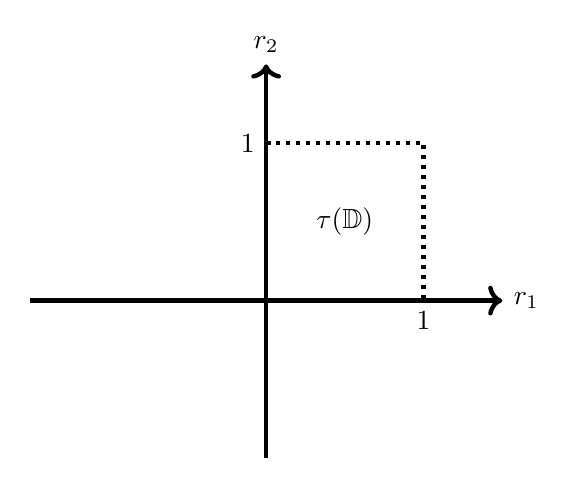
\begin{tikzpicture}
\draw[->,ultra thick] (-3,0)--(3,0) node[right]{$r_1$};
\draw[->,ultra thick] (0,-2)--(0,3) node[above]{$r_2$};
\draw[dotted, ultra thick] (0,2)node[left]{$1$} -- (2,2) -- (2,0)node[below]{$1$};
\node at (1,1) {$\tau(\mathbb{D})$};
\end{tikzpicture}
\end{center}
and 
\begin{center}
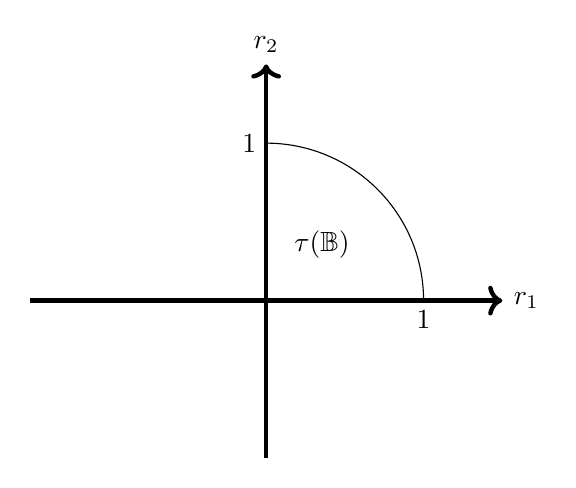
\begin{tikzpicture}
\draw[->,ultra thick] (-3,0)--(3,0) node[right]{$r_1$};
\draw[->,ultra thick] (0,-2)--(0,3) node[above]{$r_2$};
\draw (0,2)node[left]{$1$} arc[start angle=90, end angle=0, radius=2]node[below]{$1$};
\node at (0.71,0.71) {$\tau(\mathbb{B})$};
\end{tikzpicture}
\end{center}
\end{example}

\begin{definition}
Let $M\subseteq\C^n$. A function $F:M\to \C^m$ is continuous if for $F=(f_1,\cdots,f_m)$, where for each $1\leq i\leq m$, $f_i:M\to\C$, $f_i$ is continuous.
\end{definition}

\begin{definition}
$f:U\to\C$ is differentiable at $\underline{z}_0\in U$ if there exists $\Delta_i,E_i:U\to\C,(1\leq i\leq n)$ such that they are continuous at $\underline{z}_0$ and 
\begin{equation*}
f(\underline{z})-f(\underline{z}_0) = \sum_{i=1}^n (z_i-z_{0,i})\Delta_i(\underline{z})+\sum_{i=1}^n (\overline{z_i}-\overline{z_{0,i}})E_i(\underline{z}).
\end{equation*} 
$\Delta_i,E_i$ are called Wirtinger derivatives. They are usually denoted as 
\begin{equation*}
\Delta_i(\underline{z}_0) = \pd{f}{z_i}(\underline{z}_0),\quad E_i(\underline{z}_0) = \pd{f}{\overline{z_i}}(\underline{z}_0).
\end{equation*}
\end{definition}

\begin{proposition}
Let $f:U\to\C$ be differentiable. Then we have
\begin{align*}
\pd{f}{z_i} &= {\frac 1 2}\left(\pd{f}{x_i}-i\pd{f}{y_i}\right),\\
\pd{f}{\overline{z_i}} &= {\frac 1 2}\left(\pd{f}{x_i}+i\pd{f}{y_i}\right).\\
\end{align*}
\end{proposition}

\begin{corollary}
\begin{align*}
\pd{z_i}{z_j} =\delta_{ij},\quad& \pd{z_i}{\overline{z_j}} = 0,\\
\pd{\overline{z_i}}{z_j} =0,\quad& \pd{\overline{z_i}}{\overline{z_j}} = \delta_{ij}.\\
\end{align*}
In particular,
\begin{equation*}
\overline{\left(\pd{f}{z_i}\right)} = \pd{\overline{f}}{\overline{z_i}}.
\end{equation*}
\end{corollary}

\begin{definition}
Let $U\subseteq\C^n$. A function $F:U\to \C^m$ is differentiable if for $F=(f_1,\cdots,f_m)$, where for each $1\leq i\leq m$, $f_i:M\to\C$, $f_i$ is differentiable.
\end{definition}

\begin{proposition}
Let $U\subseteq\C^n$ be open. A function $f:U\to\C$ with $f=g+ih$ for some $g,h:U\to\R$ is differentiable if $g,h$ are differentiable.
\end{proposition}

\begin{proposition}[Chain Rule]
Let $U\subseteq\C^n,V\subseteq\C^m$ be open sets and consider differentiable functions $F:U\to V$ and $f:V\to \C$ where $F=(f_1,\cdots,f_m)$. We have
\begin{equation*}
\pd{(f\circ F)}{z_i}(\underline{z}) = \sum_{j=1}^m\pd{f}{w_j}(F(\underline{z}))\pd{f_j}{z_i}(\underline{z})+ \sum_{j=1}^m\pd{f}{\overline{w_j}}(F(\underline{z}))\pd{\overline{f_j}}{z_i}(\underline{z}).
\end{equation*}
\label{chain_rule}
\end{proposition}

\subsection{Holomorphic Functions}

\begin{definition}
Let $U\subseteq\C^n$ be open and $f:U\to \C$ be a function. $f$ is complex differentiable at $\underline{z}_0\in U$ if there exists functions $\Delta_1,\cdots,\Delta_n:U\to\C$ which are continuous at $\underline{z}_0$ with
\begin{equation*}
f(\underline{z})-f(\underline{z}_0) = \sum_{i=1}^n(z_i-z_{0,i})\Delta_i(z).
\end{equation*}
$f$ is holomorphic at $\underline{z}_0$ if it is complex differentiable in a neighborhood of $\underline{z}_0$. The values
\begin{equation*}
\Delta_i(\underline{z})=\pd{f}{z_i}(\underline{z}_0)
\end{equation*}
are called the complex partial derivatives. 
\end{definition}

\begin{remark}
$f$ is holomorphic at $\underline{z}_0$ if and only if it is differentiable at $\underline{z}_0$ with $E_i\equiv0$ for all $1\leq i\leq n$.
\end{remark}

\begin{example}
$z_i$ are holomorphic but $\overline{z_i}$ are not. Polynomials in $z_1,\cdots,z_n$ are holomorphic.
\end{example}

\begin{definition}
A function $F:U\to\C^m$ given by $F=(f_1,\cdots,f_m)$ is holomorphic if all $f_i$ are holomorphic.
\end{definition}

\begin{proposition}
$F:U\to\C^m$ is holomorphic if and only if for any open subset $V\subset\Image F$ and a holomorphic function $f:V\to\C$, $f\circ F$ is holomorphic.
\end{proposition}

\begin{theorem}
$f:U\to\C$ is holomorphic if and only if $f$ is real-differentiable (ie. with respect to $x_i$ and $y_i$ for $z_i = x_i+iy_i$), and for all $1\leq i\leq n$, $\pd{f}{\overline{z}_i} = 0$.
\end{theorem}

\begin{remark}
$f:U\to\C$ is holomorphic if and only if for each $1\leq i\leq n$ and fixed $z_1,\cdots,z_n$, $z_i\mapsto f(z_1,\cdots,z_n)$ is holomorphic.
\end{remark}

\begin{definition}
A complex line is a function $l:\C\to\C^n$ for some $\underline{a},\underline{w}\in\C^n,w\not=\underline{o}$, we have
\begin{equation*}
l(t) = \underline{a}+t\underline{w}.
\end{equation*}
The image of $l$ is denoted by $l(\C) = L$.
\end{definition}

\begin{notation}
For a function $f:U\to\C$, we denote \
\begin{equation*}
f|_L(t) \defeq f\circ l(t) = f(\underline{a}+t\underline{w}).
\end{equation*}
\end{notation}

\begin{remark}
Using the chain rule, we see
\begin{equation*}
{\frac d {dt}}f|_L(t) = \sum_{i=1}^n \pd{f}{z_i}(\underline{a}+t\underline{w})w_i.
\end{equation*}
\end{remark}

\subsection{Cauchy Integrals}

We will consider a holomorphic function $f:U\to\C$ where $U$ is a neighborhood of the closure of $D=D_{\underline{r}}(\underline{a})$. Without loss of generality we assume $\underline{a}=\underline{o}$. Let $\underline{z}\in D$, applying the Cauchy integral to the first variable, we see that

\begin{equation*}
f(z_1,\cdots,z_n) = {\frac 1 {2\pi i}}\int_{\vert \zeta_1\vert = r_1}{\frac {f(\zeta_1,z_2,\cdots,z_n)} {\zeta_1-z_1}}d\zeta_1.
\end{equation*}

Repeating this process, we get
\begin{equation*}
f(z_1,\cdots,z_n) = \left({\frac 1 {2\pi i}}\right)^n\int_{\vert \zeta_n\vert = r_n}\cdots\int_{\vert \zeta_1\vert = r_1}{\frac {f(\zeta_1,\cdots,\zeta_n)} {\prod_{i=1}^n(\zeta_i-z_i)}}d\zeta_1\cdots d\zeta_n.
\end{equation*}

This is valid on the disk $D$. Motivated by the above equation, we have,

\begin{definition}
The Cauchy kernel in $\C^n$ is 
\begin{equation*}
C(\underline{\zeta},\underline{z}) = \left({\frac 1 {2\pi i}}\right)^n{\frac {d\zeta_1\wedge\cdots\wedge d\zeta_n} {(\zeta_1-z_1)\cdots(\zeta_n-z_n)}}.
\end{equation*}
\end{definition}

\begin{theorem}
Let $f:\overline{D}\to\C$ be a holomorphic function and $z\in D$, we have
\begin{equation*}
f(z) = \int_T f(\underline{\zeta})C(\underline{\zeta},\underline{z}),
\end{equation*}
where $T=\partial_0D$, the distinguished boundary of the poly disk $D$. 
\label{cauchy_integral_several_variable}
\end{theorem}

\begin{proposition}
Suppose $h$ is a continuous function on $T=\partial_0D$ for some disk $D$, then the function
\begin{equation*}
F(z) = \int_Th(\underline{\zeta})C(\underline{\zeta},z),
\end{equation*}
is holomorphic on $D$
\end{proposition}

\begin{remark}
The theorem tells us that a holomorphic function $f$ on a disk $D$ is completely determined by its values on $T=\partial_0D$.
\end{remark}

\begin{remark}
The theorem also holds if the function $f$ is continuous on $\overline{D}$ and holomorphic on $D$.
\end{remark}

This theorem tells us moreover all the local properties about the holomorphic functions. The strategies are to work on the one dimensional cases or restrict functions to complex lines. All the proofs are listed in [Fi/Li, II section 1] of A Course in Complex Analysis.

\begin{theorem}
$f$ is holomorphic on an open set $U$ that is smooth. Then all the derivatives are again holomorphic. 
\end{theorem}

\begin{proof}[Sketch of the Proof]
Since an open set contains a disk, we can use the Cauchy integral on that disk. Since holomorphicness is a local property, we obtain the statement.
\end{proof}

\begin{remark}
If $f$ is as in Theorem \ref{cauchy_integral_several_variable}, then for $\underline{\alpha}\in\N_0^n$,
\begin{equation*}
D^{\underline{\alpha}} f(\underline{z}) = {\frac {\alpha_1!\cdots\alpha_n!} {(2\pi i)^n}}\int_T{\frac {f(\underline{z})} {(\zeta_1-z_1)^{\alpha_1+1}\cdots(\zeta_n-z_n)^{\alpha_n+1}}}d\zeta_1\cdots d\zeta_n.
\end{equation*}
We will denote the above formula as,
\begin{equation*}
D^{\underline{\alpha}} f(\underline{z}) = {\frac {\underline{\alpha}!} {(2\pi i)^n}}\int_T{\frac {f(\underline{z})} {(\underline{\zeta}-\underline{z})^{\underline{\alpha}+n}}}d\underline{\zeta}.
\end{equation*}
\end{remark}

\begin{theorem}[Weierstrass]
Let $(f_n)_{n\in\N}$ be a sequence of holomorphic functions uniformly converging to $f$. Then $f$ is holomorphic and all derivatives of $f_i$ are also uniformly converging to the ones of $f$.
\end{theorem}

\begin{definition}
A domain is an open connected subset of $\C^n$.
\end{definition}

\begin{theorem}[Maximal Principle]
Let $f$ be holomorphic on a domain $U$. If $\vert f\vert$ attains a local maximal then $f\equiv c$ for some constant $c\in \C$.
\end{theorem}

\begin{theorem}
Suppose $f$ is holomorphic on a closure $\overline{D}$ of some polydisk $D=D_r(\underline{z}_0)$. For $\underline{z}\in D$, 
\begin{equation*}
\left({\frac 1 {2\pi i}}\right)\int\cdots\int_T {\frac {f(\underline{z})} {(\underline{\zeta}-\underline{z})}}d\underline{\zeta}. %later
\end{equation*}
We develop this into a geometric series, and interchange the summation, we get

\begin{equation*}
f(\underline{z}) = \sum_{\alpha\in\N_0^n}a_{\underline{\alpha}}(\underline{z}-\underline{z}_0)^{\underline{\alpha}}
\end{equation*}
where for each $\underline{\alpha}\in\N_0^n$,
\begin{equation*}
a_{\underline{\alpha}} = {\frac {D^{\underline{\alpha}f(\underline{z}_0}} {\underline{\alpha}!}}.
\end{equation*}
The series is moreover uniformly convergent on $D$.
\end{theorem}

\begin{theorem}
Let $f$ be holomorphic on a domain $U$. Then for each $\underline{z}_0\in U$, there exists a convergent series
\begin{equation*}
f(z) = \sum a_{\underline{\alpha}}(\underline{z}-\underline{z}_0)^{\underline{\alpha}}
\end{equation*}
where for each $\underline{\alpha}\in\N_0^n$,
\begin{equation*}
a_{\underline{\alpha}} = {\frac {D^{\underline{\alpha}}f(\underline{z}_0)} {\underline{\alpha}!}}.
\end{equation*}
Series converges at least in the largest polydisk about $D_r(\underline{z}_0)\compembed U$ (the boundary is contained in $U$).
\end{theorem}

\begin{theorem}
Holomorphic functions are analytic, in other words, it can be locally developable into a power series.
\end{theorem}

\begin{theorem}[Identity Theorem]
  \label{identity_theorem}
If $f$ is holomorphic on a domain $U$, and it is identically $0$ in a non-empty open neighborhood $V$ in $U$, then $f$ is identically $0$ on $U$.
\end{theorem}

\begin{theorem}
Let $f$ be a continuous and holomorphic in each variable separately. Then $f$ is holomorphic. 
\end{theorem}

\begin{proof}
Can be shown using Cauchy's integral formula.
\end{proof}

\begin{definition}
Let $\mathcal{G}$ be a domain. We define $\mathcal{O}(\mathcal{G})$ to be the set of all holomorphic functions on $U$. 
\end{definition}

\begin{proposition}
$\mathcal{O}(\mathcal{G})$ is a $\C$-algebra. Furthermore, the following properties hold,
\begin{enumerate}[1).]
\item $\mathcal{O}(\mathcal{G})$ has no zero divisors. (Follows from Theorem \ref{identity_theorem}).
\item We can in %later
\end{enumerate}
\end{proposition}

\begin{proposition}
$\mathcal{O}(\mathcal{G})$ can be introduced a topology by the following way. Given a compact subset $K\subset \mathcal{G}$, we define
\begin{equation*}
V(K,\varepsilon) = \{f\in\mathcal{O}(\mathcal{G})\:|\: \vert f\vert_K<\varepsilon\}
\end{equation*}
where
\begin{equation*}
\vert f\vert_K = \max_{\underline{z}\in K}\vert f(\underline{z})\vert.
\end{equation*}
Such $V(K,\varepsilon)$ form a neighborhood basis for $0\in\mathcal{O}(\mathcal{G})$.\\
\par We observe that $\mathcal{O}(\mathcal{G})$ is a Fréchet algebra, (ie. convergence automatically means locally uniform convergence) and 
\begin{equation*}
\pd{}{z_i}:\mathcal{O}(\mathcal{G}) \to\mathcal{O}(\mathcal{G})
\end{equation*}
are continuous linear maps.
\end{proposition}

\begin{theorem}[Liouville]
Let $f$ be a bounded holomorphic function on $\C^n$. Then it is identically constant.
\end{theorem}

\begin{theorem}[Hartogs]
Let $f$ be a function which is holomorphic in each variable separately then $f$ is holomorphic.
\end{theorem}

\begin{proof}
See \cite{Hom}.
\end{proof}

\begin{theorem}[Hartogs's Kugelsatz]%later
Suppose $n>0$. Let $K\subset U$ be a compact subset of an open set such that $U\backslash K$ is connected. If $f$ is holomorphic on $U\backslash K$, then $f$ extends holomorphically to the whole $U$. 
\end{theorem}

\begin{proof}
Will be shown later.
\end{proof}

\begin{remark}
Using the theorem above, we conclude that there are no isolated singularities and isolated zeroes. (ie. a holomorphic function on a punctured domain can be extended to that point). The latter follows that if $f(\underline{z}) = 0$, then ${\frac 1 f}(\underline{z})$ has an isolated singularity.
\end{remark}

\begin{proposition}
Let $f\not\equiv0$ be a holomorphic function on a domain $\mathcal{G}$. Then the set
\begin{equation*}
V(f) \defeq \{z\in\mathcal{G}\:|\: f(z) = 0\}
\end{equation*}
has no interior points and has Lebesgue measure $0$. 
\end{proposition}

\subsection{Holomorphic Maps and Differential Forms}

For this subsection, we follow \cite{Ra}.

\begin{definition}
Let $F:\C^n\supset U\to V\subset \C^m$ be a function given by $F=(f_1,\cdots,f_m)$. It is holomorphic if $f_i$ is holomorphic for each $i$. Or equivalently for any $f\in\mathcal{O}(V)$ , the pullback $f\circ F$ is holomorphic on $U$. 
\end{definition}

\begin{corollary}
Given $U\stackrel{F}{\to}V\stackrel{G}{\to}W$ holomorphic functions, the composition $G\circ F$ is holomorphic. Obviously $\id:U\to U$ is holomorphic.
\end{corollary}

\begin{definition}
Let $U,V\subseteq\C^n$ be open and $F:U\to V$ be differentiable given by $F=(f_1,\cdots,f_n)$ such that for each $f_i$, it decomposes into
\begin{equation*}
f_i = g_i+ih_i.
\end{equation*}
We define the real Jacobian by
\begin{equation*}
J^\R_F = \begin{pmatrix}
\pd{g_i}{x_j}&\pd{h_i}{x_j}\\
\pd{g_i}{y_j}&\pd{h_i}{y_j}
\end{pmatrix}_{1\leq i,j\leq n}\in\R^{2n\times 2n},
\end{equation*}
and the complex Jacobian by
\begin{equation*}
J^\C_F = \begin{pmatrix}
\pd{f_i}{z_j}&\pd{\overline{f}_i}{z_j}\\
\pd{f_i}{\overline{z}_j}&\pd{\overline{f}_i}{\overline{z}_j}
\end{pmatrix}_{1\leq i,j\leq n}\in\C^{2n\times 2n}.
\end{equation*}
Furthermore, if $f$ is holomorphic we have the holomorphic Jacobian
\begin{equation*}
J^h_F =
\left(\pd{f_i}{z_j}\right)_{1\leq i,j\leq n}\in\C^{n\times n}.
\end{equation*}
\end{definition}

\begin{proposition}
We have the following formulas.
\begin{equation*}
\rk J^\R_F = \rk J^\C_F, \quad \det J^\R_F = \det J^\C_F. 
\end{equation*}
In particular $\det J^\C_F$ is a real number. Furthermore, if $F$ is holomorphic, 
\begin{equation*}
J^\C_F = \begin{pmatrix}
J_F^h&O\\
O& \overline{J_F^h}.
\end{pmatrix}
\end{equation*}
In particular
\begin{equation*}
\det J_F^\C = \vert\det J_F^h\vert ^2\geq 0.
\end{equation*}
\end{proposition}

\begin{proof}
exercise. %later
\end{proof}

\begin{definition}
A function $F:U\to V$ is biholomorphic if it is bijective and $F^{-1}$ is also holomorphic.
\end{definition}

\begin{proposition}
Let $F$ be a biholomorphic function, then we have
\begin{equation*}
\det J_F^\C >0.
\end{equation*}
\end{proposition}

\begin{corollary}
Biholomorphic functions preserve orientation.
\end{corollary}

Recall that if $f:U\to\C$ where $U\subset\C$ is a holomorphic and injective function. Then necessary we have $f'(z)\not=0$.

\begin{proposition}
Let $F:U\to V$ be a holomorphic bijective such that $J_F^h$ is everywhere regular (ie. its determinant is nowhere $0$). Then $f$ is biholomorphic.  
\end{proposition}

\begin{proof}
  We know that $F^{-1}$ is differentiable. We get 
  \begin{equation*}
    J_F^\C\circ J_{F^{-1}}^\C = I_{2n}.
  \end{equation*}
  By the assumption, we have,
  \begin{equation*}
    J_F^\C = \begin{pmatrix}
      M & O\\
      O & \overline{M}
    \end{pmatrix}.
  \end{equation*}
  Thus we rewrite the first equation to be 
  \begin{equation*}
      \begin{pmatrix}
      M & O\\
      O & \overline{M}
    \end{pmatrix}
    \begin{pmatrix}
      A & B\\
      C & D
    \end{pmatrix}
    =\begin{pmatrix}
      I_n & O\\
      O & I_{n}
    \end{pmatrix}
  \end{equation*}
  We have 
  \begin{align*}
    MA = E, MB = 0.
  \end{align*}
  Thus we conclude $A = M^{-1},B=O$ which gives us the Cauchy-Riemann equations.
\end{proof}

\begin{theorem}[Osgood's Theorem]
Suppose $F:U\to V$ be bijective holomorphic function where $U,V\subset\C^n$. Then $J_F^h$ is everywhere regular and $F$ is therefore biholomorphic.
\end{theorem}

\begin{proof}
\cite{Ra} chapter 2.5.
\end{proof}

\subsection{Differential Forms}

\begin{definition}
  Let $\underline{x_0}\in\R^N$. We set 
  \begin{equation*}
    \mathcal{S}(\underline{x}_0) = \{f:U_f\to\R\sep \text{ continuous function defined on some neighborhood of $\underline{x}_0$}\}
  \end{equation*}
  We can introduce an algebraic structure by for all $f,g\in \mathcal{S}(\underline{x}_0)$ and $c\in\R$,
  \begin{equation*}
    f+g:U_f\cap U_g\to\R,\quad fg:U_f\cap U_g\to\R, cf:U_f\to\R.
  \end{equation*}
  Also we define 
  \begin{equation*}
    \mathcal{D}(\underline{x}_0) = \{f\in\mathcal{S}(\underline{x}_0)\sep \text{differentiable at $\underline{x}_0$}\}.
  \end{equation*}
  A mapping $L:\mathcal{S}(\underline{x}_0)\to\R$ is linear if for any $a,b\in\R$ and $f,g\in\mathcal{S}(\underline{x}_0)$, we have 
  \begin{equation*}
    L(af+bg) = aLf+bLg.
  \end{equation*}
\end{definition}

\begin{remark}
  $\mathcal{S}(\underline{x}_0)$ is not a vector space since the additive identity is not unique.
\end{remark}

\begin{lemma}
  Let $f\in\mathcal{D}(\underline{x}_0),g\in\mathcal{S}(x_0)$ such that $f(\underline{x}_0) = 0$, then $f\cdot g\in\mathcal{D}(\underline{x}_0)$. 
\end{lemma}

\begin{proof}
  Exercise.
\end{proof}

\begin{definition}
  A linear map $D:\mathcal{D}(\underline{x}_0)\to\R$ is called a tangent vector to $\underline{x}_0\in\R^N$, if 
  \begin{enumerate}[1).]
    \item $D(1) = 0$
    \item For any $f,g\in\mathcal{D}(\underline{x}_0)$, such that $f(\underline{x}_0) = g(\underline{x}_0)=0$, then $D(fg) = 0$. 
  \end{enumerate}
\end{definition}

\begin{proposition}
  $D$ satisfies the following properties.
  \begin{enumerate}
    \item $D$ satisfies the Leipniz rule.
    \item $\pd{}{x_i}\big{|}_{\underline{x}_0}$ is a tangent vector at $\underline{x}_0$.
    \item The sets of tangent vectors at $D$ form a vector space and it has a basis consists $\pd{}{x_i}\big{|}_{\underline{x}_0}$ where $1\leq i\leq N$.
  \end{enumerate}
\end{proposition}

\begin{proof}
  Exercise. 
\end{proof}

\begin{definition}
  The vector space of tangent vectors at $\underline{x}_0$ is called the tangent space at $\underline{x}_0$ and denoted by $T_{\underline{x}_0}$. Its dual space
  is called the cotangent space and denoted by $T_{\underline{x}_0}^*$. 
\end{definition}

\begin{example}
  Let $f\in\mathcal{D}(\underline{x_0})$, we define 
  \begin{equation*}
    df:T_{\underline{x_0}}\to \R,\quad df(D) = Df,
  \end{equation*}
  is an element of the contangent space called a total differentiation.
\end{example}

\begin{proposition}
  The $dx_i$ where $i=1,\cdots, N$ is a basis for the cotangent space $T^*_{\underline{x}_0}$. Such basis is a dual basis to $\{\pd{}{x_i}\big{|}\}_{i=1,\cdots,N}$.
\end{proposition}

\begin{definition}
  Let $M\subseteq\R^N$. A Pfaffian form or ($1$-form) on $M$ associates each point $\underline{x}\in M$ to a cotangent vector $a(x)\in T^*_{\underline{x}}$. 
  From the basis of the cotangent spaces, we know 
  \begin{equation*}
    a(x) = \sum_{i=1}^N a_i(\underline{x})dx_i
  \end{equation*}
  where $a_i:M\to\R$.
  \par We call $a$ is continuous, differentiable, or measurable, if all $a_i$ are so.
\end{definition}

\begin{remark}
The set of $1$-forms on $M$ which is denoted by $E^1(M)$ is a module over $E^0(M)$, where $E^0(M)$ is a ring of functions.
\end{remark}

\begin{definition}[Exterior Products]
  $E^p(M) = \bigwedge^p E^1(M)$ module of $p$-forms, $p=0,\cdots, N$. 
  We call an element $a$ of $E^p(M)$, a $p$-dimensional differential form, which is of the form
  \begin{equation*}
    a = \sum_{\substack{I\subseteq \{1,\cdots,N\}\\\vert I\vert = p}} a_Idx^{I}.
  \end{equation*}
  where $dx^I$ denotes that 
  \begin{equation*}
    dx^I = dx_{i_1}\wedge \cdots\wedge dx_{i_N}, i_j\in I, k<l\Rightarrow i_k\leq i_l.
  \end{equation*}
  The rank of $E^p$ is ${N \choose p}$.
\end{definition}

\begin{definition}
  We define
  \begin{equation*}
    E = \bigoplus_{1\leq p\leq N}E^p.
  \end{equation*}
  The rank of $E$ is $\sum_{p=0}^N{N\choose p} = 2^N$.
\end{definition}

\begin{remark}
  Let $f$ be a differential function on an open set $M\subset\R^N$. We get a $1$-form by 
  \begin{equation*}
    M\ni x\mapsto [df(x)\in T_x^*],
  \end{equation*}
  called the total differential and this is of the form 
  \begin{equation*}
    df = \sum_{i=1}^N \pd{f}{x_i}dx_i.
  \end{equation*}
\end{remark}

\begin{definition}
  Let $a\in E^p$. $a$ is said to be sufficiently differentiable if 
  \begin{equation*}
    a = \sum_{I}a_Idx^I ,
  \end{equation*}
  then 
  \begin{equation*}
    da = \sum_I da_I\wedge dx^I \in E^{p+1},
  \end{equation*}
  where $a_I$ is a differentiable function since $a$ is differentiable. Thus we can consider the total differentiable of $a_I$.
\end{definition}

Let $a$ be a $p$-form. At each $x\in M$, we have a $p$-covector 
\begin{equation*}
  a(x) \in\bigwedge^p T_x^*.
\end{equation*}

\begin{definition}
  An exterior product is $E^p\times E^q\to E^{p+q}$ is such that 
  \begin{equation*}
    (a,b)\mapsto a\wedge b.
  \end{equation*}
  Note that we have
  \begin{equation*}
    a\wedge b = (-1)^{p+q}b\wedge a.
  \end{equation*}
  In particular, if $p$ is odd, we have,
  \begin{equation*}
    a\wedge a = 0.
  \end{equation*}
  Moreover, 
  \begin{equation*}
    dx_i\wedge dx_i = 0.
  \end{equation*}
\end{definition}

More details will be found in \cite{Lieb}Chapter 3.

\begin{theorem}
  \begin{equation*}
    d\wedge d = 0
  \end{equation*}
  and 
  \begin{equation*}
    d(a\wedge b) = da\wedge b + (-1)^pa\wedge db
  \end{equation*}
  where $a\in E^p(M)$, and whenever these expression make sense.
\end{theorem}

\begin{definition}[Transformation of Forms]

  Let $F:R^N\supseteq U\to V\subseteq \R^M$, $F=(f_1,\cdots,f_n)$ and $a\in E^p(V)$ where 
  \begin{equation*}
    a = \sum_{I}a_I dy^I.
  \end{equation*}
  We define $a\circ F$ to be 
  \begin{equation*}
    a\circ F = \sum_I a_I\circ F df^I.
  \end{equation*}
  Then this yields a $p$-form on $U$. We denote this by $F^*a$.
\end{definition}

\begin{theorem}
  \begin{equation*}
    d(a\circ F) = da\circ F.
  \end{equation*}
  In other words, total differential commutes with pullbacks.
\end{theorem}

\subsection{Integration}

\begin{definition}
  Let $M\subseteq\R^N$ and $a\in E^N(M)$ such that 
  \begin{equation*}
    a = \tilde{a}d_1\wedge\cdots \wedge d_N.
  \end{equation*}
  We define 
  \begin{equation*}
    \int_M a = \int_M \tilde{a}(x) dx_1\wedge\cdots\wedge dx_n. 
  \end{equation*}
\end{definition}

\begin{definition}
  Let $a$ be a $k$-form in $\R^N$ and $M$ be a $k$-dimensional surface on $\R^N$ such that 
  \begin{equation*}
    F:Q\to M
  \end{equation*}
  parametrizes $M$ where $Q$ is some cube.
  \begin{equation*}
    \int_M a = \int_Q a\circ F.
  \end{equation*}
\end{definition}
\begin{theorem}[Stokes]
  Let $\mathcal{G}\subset\subset\R^N$ be a relatively compact domain such that $\partial \mathcal{G}$ is $N-1$ dimensional sufficiently smooth. 
  A $N-1$-form defined and continuously differentiable on $\overline{\mathcal{G}}$, then 
  \begin{equation*}
    \int_{\partial \mathcal{G}}a = \int_{\mathcal{G}}da.
  \end{equation*}
  
\end{theorem}

\cite{Lieb} volume 3 chapter 3 integration \\
\par Now we define these notions in terms of complex analysis.

\begin{definition}
  Let $M\subset\C^n$ then $E^0_\C(M)$ denotes the $\C$-valued functions on $M$, and 
  \begin{equation*}
    E_\C^p(M) = E^p(M)\tens{E^0(M)}E^0_\C(M).
  \end{equation*}
  A $p$-form on $M$ is defined as 
  \begin{equation*}
    a = \sum_{j=1}^n a_jd_{x_j} + \sum_{j=1}^n b_jd_{y_j}
  \end{equation*}
  where $z_j = x_j+iy_j$ and $a_j,b_j$ are complex-valued functions. 
  \par If we have $f=g+ih$, then we have $df=dg+idh$. In particular ,
  \begin{equation*}
    dz_j = dx_j+idy_j,\quad d\overline{z}_j = dx_j - idy_j.
  \end{equation*}
  Thus we could write instead, 
  \begin{equation*}
    a = \sum_{j=1}^n \tilde{a}_jdz_j+\sum_{j=1}^n \tilde{b}_jd\overline{z}_j.
  \end{equation*}
\end{definition}

\begin{remark}
  Let $a\in E_\C(M)$ then 
  \begin{equation*}
    a = \sum_{r=p+1, 0\leq r\leq 2n}\sum_{\substack{1\leq i_1\leq\cdots\leq i_p\leq N\\ 1\leq j_1\leq\cdots\leq j_q\leq N}}a_{i_1,\cdots,ip,j_1,\cdots,j_q}dz_{i_1}\wedge\cdots\wedge dz_{i_p}\wedge d\overline{z}_{j_1}\wedge\cdots\wedge d\overline{z}_{j_q}.
  \end{equation*}
  This can also be written as 
  \begin{equation*}
    a = \sum_{\substack{I,J\subseteq\{1,\cdots,n\},\\\vert I\vert = p,\\ \vert J\vert = q}}a_{I,J}dz^Id\overline{z}^J.
  \end{equation*}
  Thus 
  \begin{equation*}
    E^r(M) = \bigoplus_{p+q=r}E^{p,q},
  \end{equation*}
  and
  \begin{equation*}
    E_\C(M) = \bigoplus_{r=0,\cdots,2n}E^r(M) = \bigoplus_r\bigoplus_{p,q}E^{p,q}(M).
  \end{equation*}
  The rank of $E_\C(M) = \sum{n \choose p}{n \choose q} = 2^n$.
  \par Consider 
  \begin{equation*}
    da = \sum_{I,J} da_{I,J}\wedge dz^Id\overline{z}^J,
  \end{equation*}
  In particular,
  \begin{equation*}
    da = \sum a_jdz_j + \sum b_k d\overline{z}_k,
  \end{equation*}
  for 
  \begin{equation*}
    a_j = \pd{a}{z_j},\quad b_k = \pd{a}{\overline{z}_k}.
  \end{equation*}
  Therefore 
  \begin{equation*}
    df = \partial f + \overline{\partial}f = \sum \pd{f}{z_j}dz_j + \sum \pd{f}{\overline{z}_k}d\overline{z}_k.
  \end{equation*}
  Thus we get 
  \begin{equation*}
    \partial:E^{p,q}\to E^{p+1,q}
  \end{equation*}
  and 
  \begin{equation*}
    \overline{\partial}:E^{p,q}\to E^{p,q+1}
  \end{equation*}
\end{remark}

\begin{proposition}
  From the remark above, we have the following statements.
  \begin{enumerate}[1).]
    \item $d = \partial +\overline{\partial}$,
    \item $d\circ d = 0$, $\partial\overline{\partial}+\overline{\partial}\partial = \partial\circ\partial = \overline{\partial}\circ\overline{\partial}= 0$.
    \item Let $f$ be a function, $f$ is holomorphic if and only if $\overline{\partial}f=0$
    \item Commutativity for $\wedge$ holds.
    \item Leipniz rules hold for $\partial (f\wedge g)$.
  \end{enumerate}
\end{proposition}

\begin{example}
  \begin{equation*}
    dx_1\wedge dy_1\wedge\cdots\wedge dx_n\wedge dy_n = -\left({\frac 1 {n}}\right)^n dz_1\wedge d\overline{z}_1\wedge\cdots\wedge dz_n\wedge d\overline{z}_n.
  \end{equation*}
  This is called the volume form $dV$. 
  \begin{equation*}
    \int_MdV = \int_M d\lambda(z) = \lambda(M),
  \end{equation*}
  where $\lambda$ is the Lebesgue measure.
\end{example}

\begin{example} Recall the Cauchy kernel.
  \begin{equation*}
    C(\underline{\zeta},\underline{z}) = \left({\frac 1 {2\pi i}}\right)^n {\frac {d\underline{\zeta}} {(\underline{\zeta}-\underline{z})}}.
  \end{equation*}
  This is a form of type $(n,0)$ in $\underline{\zeta}$ defined on the open set
  \begin{equation*}
    \C^n\times \C^n - \Delta,
  \end{equation*}
  where $\Delta = \{(\underline{\zeta},\underline{z})\sep \forall j=1,\cdots,n \zeta_j = z_j\}$.
\end{example}\

\begin{proposition}[Transformation Rules]
  Let $F:U\to V$ be holomorphic where $U\subset\C^n$ and $V\subset\C^m$. For $a\in E^{p,q}(V)$, 
  \begin{equation*}
    a\circ F = \left(\sum_{I,J} a_{I,J} dw^I\wedge d\overline{w}^J\right)\circ F  = \sum_{I,J} a_{I,J}\circ F (dw^I\circ F)\wedge (d\overline{w}^J\circ)
  \end{equation*}
  where $F=(f_1,\cdots f_n)$ and 
  \begin{equation*}
    dw_j\circ F = d(w_j\circ F)=df_j
  \end{equation*}
  for each $j$ and similarly for $d\overline{w}_j$. 
  \par In particular, we have $a\in E^{p,q}(V)$, $a\circ F \in E^{p,q}(U)$. If $F$ is just differentiable we get $a\circ F\in E^{p+q}(U)$.
\end{proposition}

\begin{proposition}
  Let  Let $F:U\to V$ be differentiable and $a\in E^{p,q}(V)$, we have 
  \begin{equation*}
    d(a\circ F) = da\circ F. 
  \end{equation*}
  Furthermore, if $F$ is holomorphic, we have,
  \begin{equation*}
    \partial (a\circ F) = \partial a\circ F, \overline{\partial}(a\circ F) = \overline{\partial} \circ F.
  \end{equation*}
\end{proposition}

\begin{definition}[Poincaré Equation]
  Let $\mathcal{G}\subseteq\R^N$ be a domain and $f\in E^r$ such that $df = 0$. The equation 
  \begin{equation*}
    du = f,
  \end{equation*}
  is called the Poincaré equation.
\end{definition}

\begin{definition}
  Let $a\in E^r$. $a$ is called
  \begin{enumerate}[1).]
    \item a closed form if $da = 0$.
    \item an exact form if there exists $u\in E^{r-1}$ such that $du = a$.
  \end{enumerate}  
\end{definition}

\begin{theorem}
  If the domain is convex in the above then the Poincaré equation is solvable. (ie. all the de Rham cohomologies are $r=0$ except the $0$ temr.)
  \par Furthermore,
  \begin{equation*}
    Z^r = \{f\in E^r\sep df = 0\},
  \end{equation*}
  \begin{equation*}
    B^r = \{du\sep u\in E^{r-1}\}.
  \end{equation*}
  We have $B^r\subset Z^r$, $H_{dR}^r(\mathcal{G}) = Z^r/B^r$, gives the de Rham cohomology and 
  \begin{equation*}
    H_{dR}^0(\mathcal{G}) = \C,
  \end{equation*}
  if $r\not=0$, then 
  \begin{equation*}
    H_{dR}^r(\mathcal{G}) = 0.
  \end{equation*}
  Note that $B^0$ is empty as there is no such thing as $-1$-form.
\end{theorem}

\begin{definition}
  Let $\mathcal{G}\subset\C^n$, $f\in E{p,q}$. Consider the equation,
  \begin{equation*}
    \overline{\partial}u = f \quad u\in E^{p,q-1}.
  \end{equation*}
  If such equation holds, then we necessarilyhave $\overline{\partial}f = 0$. We get 
  \begin{equation*}
    \overline{\partial}u = f, \overline{\partial}f = 0
  \end{equation*}
  in $\mathcal{G}$. We define similarly,
  \begin{align*}
    Z^{p,q} &= \{f\in E^{p,q}\sep \overline{\partial}f = 0\},\\
    B^{p,q} & = \{\overline{\partial}u \sep u\in E^{p,q-1}\},\\
    H^{p,q}_{dR}(\mathcal{G})=Z^{p,q}/B^{p,q}\\
  \end{align*}
  This cohomology is called Dolbeault cohomology. This gives 
  \begin{equation*}
    H^{0,0}(\mathcal{G}) = \mathcal{O}(\mathcal{G})
  \end{equation*}
  the sheaf of holomorphic functions.
\end{definition}

\subsection{Bochner-Martinelli Integral Formulas}

\begin{definition}
  We define the form 
  \begin{equation*}
    \beta = \beta(\underline{\zeta},\underline{z}) = \sum_{j=1}^n (\overline{\zeta}_j-\overline{z}_j)d\zeta_j.
  \end{equation*}
  We also define 
  \begin{equation*}
    B(\underline{\zeta},\underline{z}) = \left({\frac 1 {2\pi i}}\right){\frac {1} {\norm{\underline{\zeta}-\underline{z}}^{2n}}}\beta\wedge(\overline{\partial}_\zeta\beta)^{n-1},
  \end{equation*}
  where 
  \begin{equation*}
    \overline{\partial}_{\underline{\zeta}}\beta = \sum_{j=1}^n d\overline{\zeta}_j\wedge d\zeta_j = \sum_{j=1}^n \omega_j
  \end{equation*}
  where $\omega_j = d\overline{\zeta}_j\wedge d\zeta_j$ and the power means the exterior product. 
  This $B$ above is called the Bochner-Martinelli formel which is define on $\C^n\times \C^n$ except the diagonall. 
\end{definition}

\begin{remark}
  For $n=1$, we have 
  \begin{equation*}
    B = {\frac 1 {2\pi i}}{\frac 1 {(\zeta-z)(\overline{\zeta}-\overline{z})}}(\overline{\zeta}-\overline{z})d\zeta = {\frac 1 {2\pi i}}{\frac {d\zeta} {\zeta - z}}.
  \end{equation*}
\end{remark}

\begin{remark}
  Given a $(n,n-1)$ form in $\zeta$ which is a function in $z$. 
\end{remark}

\begin{lemma}
\begin{equation*}
  d_\zeta B(\mzeta, \mz) = \overline{\bd}_\zeta B(\mzeta,\mz) = 0.
\end{equation*}
\end{lemma}
\begin{proof}
  For $\mz=0$, we get 
  \begin{equation*}
    \beta = \sum_j \czeta_j d\zeta_j,\quad \omega^j = d\cz_j\wedge d\zeta_j.
  \end{equation*}
  If $K\subset\{1,\cdots,n\}=N$, then 
  \begin{equation*}
    \omega^K = \bigwedge_{j\in K}\omega^j.
  \end{equation*}
  We already know,
  \begin{equation*}
    \overline{\bd}\beta = \sum \omega_j,
  \end{equation*}
  and 
  \begin{equation*}
    (\overline{\bd}\beta)^k = \left(\sum \omega_j\right) = k!\sum_{|K|=k}\omega^K.
  \end{equation*}
  Furthermore,
  \begin{equation*}
    \overline{\bd}_\zeta\norm{\mzeta}^2 = \overline{\bd}\sum \czeta_j\zeta = \sum \zeta_j d\czeta_j = \overline{\beta}. 
  \end{equation*}
  \begin{align*}
    (2\pi i)^n\overline{\bd}B(\mzeta,\mz) &= \overline{\bd}(\beta\wedge(\overline{\bd})^{n-1}{\frac 1 {\norm{\zeta}^{2n}}})\\
    & = {\frac {-n\overline{\beta}} {\norm{\mzeta}^{2n+2}}}\wedge\beta\wedge(\overline{\bd_\zeta}\beta)^{n-1}+{\frac 1 {\norm{\zeta}^{2n}}}(\overline{\partial}\beta)^n\\
    & = {\frac 1 {\norm{\zeta}^{2n}}}\left[{\frac {-n\overline{\beta}\wedge\beta} {\norm{\zeta}^2}}+\overline{\partial}\beta\right]\wedge(\overline{\bd}\beta)^{n-1}.
  \end{align*}
  In particular,
  \begin{equation*}
    \overline{\beta}\wedge\beta = \sum_{j,k}\zeta_j\czeta_k d\czeta_j\wedge d\zeta_k = \sum_{j\not=k}\zeta_j\czeta_kd\czeta_j d\zeta_k+\sum \vert\zeta_j\vert^2d\omega_j.
  \end{equation*}
  Thus we get 
  \begin{equation*}
    \overline{\beta}\wedge\beta\wedge(\overline{\bd}_\zeta\beta)^{n-1} = 0+\sum \vert\zeta_j\vert^2\omega_j(n-1)!\sum_{k=1}^n\omega^{N+k}=(n-1)!\sum_{j=1}^n\vert\zeta_j\vert^2\omega^N = (n-1)!\norm{\mzeta}^2\omega^N.
  \end{equation*}
  \begin{equation*}
    (2\pi i)^n\overline{\bd}B(\mzeta,0) = {\frac 1 {\norm{\mzeta}^{2n}}}\left[-n!\omega^N+n!\omega^N\right] = 0.
  \end{equation*}
\end{proof}

\begin{theorem}
  Let $\mathcal{G}\subset\subset \C^n$ with $\partial \mathcal{G}$ is reasonable (ie. the Stoke's theorem holds.) Let $f\in\mathcal{C}^1(\overline{\mathcal{G}})$, and $z\in\G$. We have 
  \begin{equation*}
    f(z) = \int_{\partial \G}f(\underline{\zeta})B(\underline{\zeta},\underline{z}) - \int_\G \overline{\partial}f(\underline{\zeta})\wedge B(\underline{\zeta},\underline{z}).
  \end{equation*}
  The special case is that for $n= 1$, we have, 
  \begin{equation*}
    f(z) = {\frac 1 {2\pi i}}\int_{\partial B} {\frac {f(\zeta)} {\zeta-z}}d\zeta + {\frac 1 {2\pi i}}\int_\G \pd{f(\zeta)}{\overline{\zeta}}{\frac 1 {\zeta-z}}d\zeta\wedge d\overline{\zeta}.
  \end{equation*}
\end{theorem}
\begin{proof}
  Observe that $B$ has a singularity of order ${\frac 1 {\norm{\zeta-z}^{2n-1}}}$ in $\C^n\cong\R^{2n}$ since $\beta$ consists of linear terms.
  Using the Lemma above, we get and denote $\G_\varepsilon = \G\backslash\overline{B(z,\varepsilon)}$ for sufficiently small $\varepsilon>0$. 
  \begin{align*}
    \int_{\G_\varepsilon} \overline{\bd}f(\mzeta)\wedge B(\mzeta,\mz) &= \int_{\G_\varepsilon}\overline{\bd}(f(\mzeta)B(\zeta,z)),\\
    & = \int_{\G_\varepsilon}d_\zeta(f(\mzeta)B(\mzeta,\mz)),\\
    & = \int_{\bd\G_\varepsilon}f(\mzeta)B(\mzeta,\mz),\\
    & = \int_{\bd\G}f(\mzeta)B(\mzeta,\mz)-\int_{\bd B(z,\varepsilon)}f(\mzeta)B(\mzeta,\mz).
  \end{align*}
  Taking $\varepsilon\to0$, we get 
  \begin{equation*}
    \int_\G\overline{\bd}f\wedge B = \int_{\bd\G}f(\mzeta)B(\mzeta,\mz)-\lim_{\varepsilon\to 0 }\int_{\bd B(z,\varepsilon)}f(\mzeta)B(\mzeta,\mz).
  \end{equation*}

\end{proof}

\begin{remark}
  In $\R^n$ and $\alpha<n$, we have 
  \begin{equation*}
    \int_{B(0,R)}{\frac {dV} {r^\alpha}}<\infty,
  \end{equation*}
  and if $\alpha>n$, we have 
  \begin{equation*}
    \int_{\R^n\backslash B(0,R)}{\frac {dV} {r^\alpha}}<\infty,
  \end{equation*}
  but if $\alpha=n$, neither of them exsits.
\end{remark}

\begin{lemma}
  Let us define,
  \begin{equation*}
    B^1(\mzeta,\mz) = (n-1)\left({frac 1 {2\pi i}}\right)^n{\frac 1 {(\norm{\mzeta-\mz})^{2n}}}\beta\wedge(\overline{\partial_\zeta}\beta)^{n-2}\overline{\partial_z}\beta
  \end{equation*}
  Then we have 
  \begin{equation*}
    \overline{\zeta}_zB(\mzeta,\mz) = \overline{\partial}_\zeta B^1(\mzeta,\mz).
  \end{equation*}
  \label{lemma_4_3}
\end{lemma}

Let $\mathcal{G}$ be a domain and consider a ball $B(z,\varepsilon)$ inside $\mathcal{G}$. We know that 
\begin{equation*}
  \int_\mathcal{G}\overline{\partial}f(\zeta)\wedge B(\zeta,z) = \int_{\bd\mathcal{G}}f(\zeta)B(\zeta,z) - \lim_{\varepsilon\to 0}\int_{S_{\varepsilon}}f(\zeta)B(\zeta,z).
\end{equation*}

Examine the last term,
\begin{equation*}
  \int_{S_\varepsilon}f(\zeta)B(\zeta,z) = \left({\frac 1 {2\pi i}}\right)^{n}{\frac 1 {\varepsilon^{2n}}}\int_{\bd\mathcal{G}}f(\zeta)\tilde{B}(\zeta,z),
\end{equation*}
where
\begin{equation*}
  \tilde{B}(\zeta,z) = \beta\wedge(\overline{\partial}\beta)^{n-1}.
\end{equation*}
That is 
\begin{equation*}
  \int_{S_\varepsilon}f(\zeta)\tilde{B}(\zeta,z) = \int_{S_\varepsilon}(f(\zeta)-f(z))\tilde{B}(\zeta,z)+f(z)\int_{S_\varepsilon}\tilde{B}(\zeta,z).
\end{equation*}
Call the integrals on the right hand side $I_1,I_2$, respectively. 
\par Clearly we have,
\begin{equation*}
  \vert I_1\vert \leq\max_{\zeta\in B_\varepsilon}\vert f(\zeta)-f(z)\vert c_1\cdot\varepsilon\cdot c_2\cdot \varepsilon^{2n-1},
\end{equation*}
where the constants $c_1$ depends on $\beta$ and $c_2$ depends on .%later
Furthermore,
\begin{equation*}
  \leq c_1c_2\varepsilon^{2n}\max\vert f(\zeta)-f(z)\vert.
\end{equation*}
Therefore, the upper bound can be 
\begin{equation*}
  \left\vert {\frac 1 {2\pi i}}{\frac 1 {\varepsilon^{2n}}}I_1\right\vert\leq c\max\vert f(\zeta)-f(z)\vert.
\end{equation*}
By the continuity, we have $\varepsilon\to0$, then $\zeta\to z$ thus $I_1$ vanishes as we take the limit.
\par For the another term, by applying Stoke's theorem, 
\begin{equation*}
  I_2 = f(z)\int_{S_{\varepsilon}} \tilde{B}(\zeta,z) = f(z)\int_{B_\varepsilon}d_\zeta \tilde{B}(\zeta,z).
\end{equation*}
Substituting the definition of $\tilde{B}$, we get,
\begin{equation*}
  = f(z)\int_{B_\varepsilon}(\overline{\partial}\beta)^n.
\end{equation*}
Furthermore,
\begin{equation*}
  \overline{\partial}\beta = \sum_j\overline{\zeta}_j\wedge d\zeta_j = \sum_j\omega_j.
\end{equation*}
Thus we obtain,
\begin{equation*}
  f(z)n!\int_{B_\varepsilon}\omega_1\wedge\cdots\wedge\omega_n = n!\int_{B_\varepsilon}d\Vol(2\pi i)^n = n!{\frac {\pi^n} {n!}}\varepsilon^{2n}(2 i)^n = (2\pi i)^n\varepsilon^{2n}.
\end{equation*}
Thus taking $\varepsilon\to 0$, we get 
\begin{equation*}
  I_2\to f(z)\int_{S_\varepsilon}B(\zeta,z) = f(z).
\end{equation*}
\begin{theorem}
  Let $\mathcal{G}$ be a domain with $\bd\mathcal{G}$ resonable. \\
  \par If $f$ is holomorphic on $\overline{\mathcal{G}}$, then for any $z\in\mathcal{G}$, we have 
  \begin{equation*}
    f(z) = \int_{\bd\mathcal{G}}f(\zeta)B(\zeta,z).
  \end{equation*}
  \par If $f$ is holomorphic on a neighborhood $U$ of $\mathcal{G}$, then we have 
  \begin{equation*}
    F(z) = \int_{\partial\mathcal{G}}f(\zeta)B(\zeta,z),
  \end{equation*}
  is holomorphic on $\mathcal{G}$.
\end{theorem}
\begin{proof}
We compute the Following
\begin{equation*}
  \overline{\partial}_zF(z) = \int_{\partial\mathcal{G}}f(\zeta)\overline{\partial}_zB(\zeta,z).
\end{equation*}
By Lemma \ref{lemma_4_3}, we get 
\begin{align*}
  & = \int_{\partial\mathcal{G}}f(\zeta)\overline{\partial}_\zeta B^{1}(\zeta,z),\\
  & = \int_{\partial\mathcal{G}}\overline{\partial}_\zeta(f(\zeta)B^1(\zeta,z)),\\
  & = \int_{\partial\mathcal{G}}d_\zeta(f(\zeta)B^1(\zeta,z)),\\
  & = \int_{\partial\partial\mathcal{G}}\cdots = 0.
\end{align*}
The last equality follows from the exactness.
\end{proof}
\begin{theorem}[Hartogos' Kugelsatz or Hartogos' Ball Theorem]
  For $n>1$, let $U\subset\C^n$ be open and $K\subset U$ be compact. Assume $U,K$ are both connected. If $f$ is holomorphic on $U\backslash K$, there is $F$ on $U$ such that 
  \begin{equation*}
    F|_{U\backslash K} = f.
  \end{equation*}
  In other words, $f$ extends holomorphically to the whole $U$. 
\end{theorem}
\begin{proof}
  Let $\G_0,\G$ be domains such that $K\subset \G_0\subset \G$ and $\G_0,\G$ have reasonable boudaries. Let $z\in \G\backslash\overline{\G_0}$. Using Bochner-Martinelli, we get 
  \begin{equation*}
    f(z) = \int_{\bd\G} f(\zeta)B(\zeta,z) - \int_{\bd\G_0}f(\zeta)B(\zeta,z) = F_1(z) - F_2(z).
  \end{equation*}
  Let us denote the two integral terms on the right hand sides $F_1(z),F_2(z)$, respectively.
  $F_1$ is holomorphic in $z$ on $\G$, and $F_2$ is holomorphic in $z$ on $\C^n\backslash\G_0$. 
  \par Let $L$ be a complex line such that $L\cap\G_0=\overline{\emptyset}$. By construction,
  \begin{equation*}
    F_2(z) = \int{\frac {\text{something bounded}} {\norm{\zeta-z}^{2n}}}\norm{\zeta-z}\to 0,
  \end{equation*}
  as $z\to \infty$ under the assumption $n>1$. Restating $z\to\infty\Rightarrow F_2(z)\to0$.
  \par Observe that $F_2|L \equiv 0$, by Liouville's theorem using the single variable complex analysis. In general, $F_2\equiv 0$ on any open subsets $U\backslash K$. 
  By the connectedness, we conclude $F_2\equiv0$ on $U\backslash K$. 
  \par Thus we conclude that 
  \begin{equation*}
    F_1  \equiv f\text{ on } \G\backslash K
  \end{equation*}
  yields the holomorphic extension.
\end{proof}
\begin{corollary}
  There are no isolated singularities nor isolated zeros for $n > 1$.
\end{corollary}
\begin{proof}
  Suppose a function $f$ has a singularity at $z_0$. Suppose $f$ is holomorphic on $U\backslash \{z_0\}$. By the theorem above and $\{z_0\}$ is compact, we see $f$ can be holomorphically extended to $U$. We derived a contradiction.
  \par Similarly, if $f$ has $0$ at $z_0$ and ${\frac 1 f}$ is holomorphic on $U\backslash\{z_0\}$, then by the same argument, we derived a contradiction.
\end{proof}

\begin{remark}[Caution!!]
\par Suppose we are given a holomorphic function $f$ on variable at least $2$, such that 
\begin{equation*}
  f = g+ ih.
\end{equation*}
where $g,h:\R^2n\to\R$. Then 
\begin{equation*}
  V(f) = V(g)\cap V(h),
\end{equation*}
where $V(f)$ denotes the set of zeros of $f$. Observe that $V(g),V(h)$ are $2n-1$ dimensional sets thus the intersection is $2n-2$ unless they do not coincide.
\end{remark}

\begin{theorem}[Cauchy/Pmperi ]
  Let $\G$ be a domain with a resonable boundary $\bd\G$ such that $\G\subset\subset \C$. Let $f\in\mathcal{C}^1(\overline{G})$. For $z\in\G$, we have 
  \begin{equation*}
    f(z) = {\frac 1 {2\pi i}}\int_{\bd\G}{\frac {f(\zeta)} {\zeta-z}}d\zeta + {\frac 1 {2\pi i}}\int_\G{\frac{\pd{f}{\overline{\zeta}}(\zeta)} {\zeta-z}}d\zeta\wedge d\overline{\zeta}.
  \end{equation*}
  Apply $f\in \mathcal{C}^1(\overline{G})$, and solve,
  \begin{equation*}
    \pd{u}{\overline{z}} = f.
  \end{equation*}
\end{theorem}

\begin{proof}
  Assume $u$ is a solution $\in\mathcal{C}(\overline{\G})$, 
  \begin{equation*}
    u(z) = {\frac 1 {2\pi i}}\int_{\bd\G}{\frac {u(\zeta)}{\zeta-z}}d\zeta + {\frac 1 {2\pi i}}\int_\G{\frac {f(\zeta)} {\zeta-z}}d\zeta\wedge d\overline{\zeta}.
  \end{equation*}
  By the assumption, we get 
  \begin{equation*}
    f(z)  = \pd{u}{\overline{z}}=\pd{}{\cz}{\frac 1 {2\pi i}}\int_\G {\frac {f(\zeta)} {\zeta -z }}d\zeta\wedge d\overline{\zeta}.
  \end{equation*}
\end{proof}
\begin{theorem}
  Let $\G,\bd\G$ as before in $\C$. Suppose $f\in\mathcal{C}^1(\G)\cap L^1(\C)$. Then there is a solution $u\in\mathcal{C}^1(\G)$ such that $u$ solves,
  \begin{equation*}
    \pd{u}{\overline{z}} = f.
  \end{equation*}
\end{theorem}

For $n>1$, and $\G,\bd\G$ a domain with a reasonable boundary. We see $f\in\mathcal{C}^1_{0,1}(\overline{\G})$, $\overline{\partial}f = 0$. We get 
\begin{equation*}
  \overline{\partial}u = f.
\end{equation*}

Suppose such $u$ exists. By Bochner-Martinelli, we get 
\begin{equation*}
  u(z) = \int_{\bd\G}u(\zeta)B(\zeta,z) - \int_\G f(\zeta)\wedge B(\zeta,z).
\end{equation*}

Then we get 
\begin{equation*}
  f = \overline{\partial} u = \overline{\partial}\int_{\bd\G}\cdots-\partial\int_\G\cdots.
\end{equation*}
However, the first integral term on the right hand side does not equal $0$. 

\subsection{Hartogos Levi problems.}

The first problem is, given $n>1$, there exists adomain $\G$ such that all holomorphic functions on $\G$ extends holomorphically to a larger domain.
\par Characterize the domains where this does not happen. 
\begin{definition}
  A domain of holomorphy is a domain such that there exists a holomorphic function on it which cannnot be extended holomorphically to a larger domain.
\end{definition}

The second problem is that if $\G$ is a domain of holomorphy, can we have a function theory there?

\begin{example}
  $\C$ is a domain of holomorphy as it cannnot be extended to a larger domain. Let $f_1,f_2$ be entire function which are holomorphic in $\C$ which do not have common zeros.
  \par Solve the Diophantine equation,
  \begin{equation*}
    g_1f_1 +g_2f_2 \equiv 1. 
  \end{equation*} 
  The solutions indeed exists. Assume that the zeros $\{a_1,\cdots\}$ of $f_2$ are simple and set 
  \begin{equation*}
    c_i = f_1(a_i).
  \end{equation*}
  Find $g_1$ with 
  \begin{equation*}
    g_1(a_i) = {\frac 1 {c_i}}.
  \end{equation*}
  Set $g_2$ to be 
  \begin{equation*}
    g_2 = {\frac {1 - g_1f_1} {f_2}}.
  \end{equation*}
\end{example}

\begin{example}
  Let $\G=\C^2\nonzero$, Let us define 
  \begin{equation*}
    f_1 = z_1, f_2 = z_2. 
  \end{equation*}
  If we have 
  \begin{equation*}
    g_1z_1+g_2z_2 = 1
  \end{equation*}
  on $\G$.
\end{example}

The third problem is 
Study the zero set of holomorphic function. This leads to analytic sets.

\section{Power Series}

\subsection{Generalities}
\begin{notation}
  We will use the following conventions.
  \begin{enumerate}[1).]
    \item $\N_0 = \N\cup\{0\}$
    \item $\N_0^n = \{\alpha = (\alpha_1,\cdots,\alpha_n)\sep 1\leq i\leq n,\alpha_i \in\N_0\}$
    \item $z = (z_1,\cdots,z_n)$
    \item For $\alpha\in \N_0^n$, $z^\alpha = \prod_{i=1}^n z_i^{\alpha_i}$
    \item $\vert\alpha\vert = \sum_{i=1}^n\alpha_i$.
    \item $f = f(z) = \sum_{\alpha\in\N_0^n}a_\alpha z^\alpha$
  \end{enumerate}
\end{notation}
\begin{definition}
  We define the formal power series as 
  \begin{equation*}
    f = \sum_{j\in\N_0}f_j,
  \end{equation*}
  where $f$ is homogeneous polynomial of degree $j$. The sums and products are given by 
  \begin{equation*}
    f+g = \sum_{i\in\N_0}f_i+g_i,\quad fg = \sum_{i=0}^n \sum_{j+k=i}f_jg_k.
  \end{equation*}
  The ring of formal power series with the above operation over a commutative ring $\C$ is denoted by 
  \begin{equation*}
    \C\llbracket z\rrbracket.
  \end{equation*}
\end{definition}
\begin{definition}
  Let $f=\sum_{i\in\N_0}f_i$, then we define the order of $f$ to be the minimum index $i$ such that $f_i \not = 0$.
  We will denote this by $\order(f)$.
\end{definition}
\begin{proposition}
  Let $f,g\in\C\llbracket z\rrbracket$, we have 
  \begin{enumerate}[1).]
    \item $\order(f)\geq 0$ for any non-zero element. Moreover $\order(f) = 0$ if and only if $f$ is a unit.
    \item $\order(f) = \infty \Leftrightarrow f\equiv 0$
    \item $\order(fg) = \order(f)+\order(g)$
    \item $\order(f+g) \geq \min\{ \order(f),\order(g)\}$
  \end{enumerate}
  It follows that $\C\llbracket z \rrbracket$ is an integral domain.
\end{proposition}

\begin{corollary}
  $\C\llbracket z\rrbracket$ has a unique maximal ideal.
  \begin{equation*}
  \mathfrak{m} = \{f\in\C\llbracket z\rrbracket\sep \order(f)>0\}.
  \end{equation*}
\end{corollary}

\begin{definition}[Convergent Power Series]
  For any $\underline{r}\in\N_0^n$, we define $c_{\underline{r}}\in\C$, then 
  \begin{equation}
    \sum_{\underline{r}\in\N^n_0}c_{\underline{r}}
  \end{equation}
  converges to $c\in \C$ if for any $\varepsilon>0$, there is a finite subset $J_0\subset\N_0^n$ such that for all finite $j\subset\N_0^n$, with $ J\supset J_0$ we have,
  \begin{equation}
    \left\vert\sum_{\underline{r}\in J} c_{\underline{r}}-c\right\vert <\varepsilon.
  \end{equation}
\end{definition}

\begin{proposition}
  The convergence of the series implies the absolute, unconditional convergence, and uniform convergence.
\end{proposition}

\begin{definition}
  Let $c_{\underline{r}}$ be a function on $M$ then 
  \begin{equation}
    \sum_{\underline{r}\in\N_0^n}c_r \stackrel{\Rightarrow}{M} c
  \end{equation}
  if and only if for any $\varepsilon>0$, there exists a finite set $J_0\subset\N_0^n$ such that for all finite set with $J\supset J_0$,
  and all $x\in M$, we have 
  \begin{equation}
    \left\vert\sum_{\underline{r}\in J}c_{\underline{r}}(x)-c(x)\right\vert <\varepsilon.
  \end{equation}
\end{definition}

\begin{example}[Geometric Series]
  Let $0\leq q_i\leq 1$ for $i=1,\cdots,n$, then 
  \begin{equation}
    \sum_{\underline{r}\in\N_0^n}\prod_{i=1}^n q_i^{r_i} = \prod_{i=1}^n{\frac 1 {1-p_i}}.
  \end{equation}
\end{example}

\begin{proposition}
  Let 
  \begin{equation*}
    f = \sum_{\underline{r}\in\N_0^n}a_{\underline{r}z^{\underline{r}}}\in\C\llbracket z\rrbracket.
  \end{equation*}
  Take
  \begin{equation*}
  \underline{z}_0 = (z_{0,1},\cdots ,z_{0,n})\in\C^n, z_j^0\not=0.
  \end{equation*}
  Then if there exists $S>0$ such that 
  \begin{equation}
    \vert a_{\underline{r}}z_0^{\underline{r}}\vert\leq S,
  \end{equation}
  then $f(z)$ converges for all $\underline{z}$ with 
  \begin{equation*}
    \forall j, \vert z_j\vert \leq z_{0,j}.
  \end{equation*}
  Converges uniformly for all $\underline{z}$ such that there exists $r_j>0$ with
  \begin{equation*}
    \vert z_j\vert \leq r_j<\vert z_{0,j}\vert.
  \end{equation*}
\end{proposition}
\begin{corollary}
  A sum of power series is holomorphic function.
\end{corollary}

\begin{remark}[Warning]
  If $f\in\C\llbracket z\rrbracket$, the domain of covergence is equal to the interior of the set of convergence. 
\end{remark}

\begin{example}
  Let
  \begin{equation*}
    f(z_1,z_2) = z_2\sum_{i=1}^\infty z_1^i.
  \end{equation*}
  Then the set of convergence is 
  \begin{equation*}
    \{(z_1,z_2)\sep z_2=0\}\cup\{(z_1,z_2)\sep \vert z_1\vert <1\}.
  \end{equation*}
  The domain of convergense is 
  \begin{equation*}
    \{\vert z_1\vert < 1\}.
  \end{equation*}
\end{example}

\begin{definition}
  The convergence set is logarithmetically convex complete Reinhardt domain.
\end{definition}

Gr/FR Einfuhrung Ch I.

\begin{definition}
  We define the ring of convergent power sereis to be 
  \begin{equation*}
    \C\{z_1,\cdots,z_n\}\subset\C\llbracket z_1,\cdots,z_n\rrbracket,
  \end{equation*}
  which consists of those formal power series whose domain of convergence contains some neighborhood around the origin.
\end{definition}
\begin{remark}
  This inherits the properties from $\C\llbracket z_1,\cdots,z_n\rrbracket$, namely, it is an integral domain, which is local with unique maximal ideals
  \begin{equation*}
    \mathfrak{m} = \{f\sep f(0) = 0\},
  \end{equation*}
  and units are the one such that $\order(f) = 0$.
\end{remark}

\begin{remark}
  It is clear that if $f$ is a unit then there exists $g\in\C\{z_1,\cdots,z_n\}$ such that $fg = 1$. Therefore,
  \begin{equation*}
    \order(f)+\order(g) = \order(1) = 0.
  \end{equation*}
  Therefore $\order(f) = 0$. if $f$ is holomorphic at $0$ and $f(0)\not= 0$. Then ${\frac 1 f}$ is also holomorphic at $0$, there for taking the taylor series of ${\frac 1 f}$ to be $g$, we obtain the desired unit.
\end{remark}

\begin{remark}
  For $n=1$, we get, 
  \begin{equation*}
    (a_0+a_1z+\cdots)(b_0+b_1z+\cdots) = 1,
  \end{equation*}
  where $a_0\not=0$.
\end{remark}

\begin{definition}
  Let $z\in\C^n$, $f,g$ be holomorphic functions defined in $z$. We denote $f\cong g$ if $f$ coincides with $g$ on some neighborhood of $z$. Such equivalence classes are called the germs of holomorphic functions.
\end{definition}

\begin{definition}
  The ring of germs at $z_0\in\C^n$ which is denoted by $\mathcal{O}_{z_0}$ is isomorphic to $\C\{z-z_0\} \cong \C\{z\}$.
\end{definition}

\begin{definition}
  If $f$ is a holomorphic function on $U$ and $z\in U$. The germ of $f$ at $z$ is denoted by $f_z$ or $\gamma_z f$ (ie. an equivalence class which is represented by the taylor series of $f$ around $z$).
\end{definition}

\begin{remark}
  Let $\mathcal{D}_z$ be the ring of smooth funtions defined arond $z$ and $\mathcal{C}_z$ be the continuous function defined around $z$, then we have 
  \begin{equation}
    \mathcal{O}_z\subset\mathcal{D}_z\subset\mathcal{C}_z.
  \end{equation}
\end{remark}

\begin{definition}
  The sheaf of holomorphic function is defined to be 
  \begin{equation*}
    \mathcal{O} = \bigsqcup_{z\in\C^n}\mathcal{O}_z,
  \end{equation*}
  together with a canonical projection $p:\mathcal{O}\to \C^n$.
\end{definition}

\begin{definition}
  A (continuous) section in $\mathcal{O}$ corresponding to an open set $U\subset \C^n$ is such that 
  \begin{equation}
    \sigma:U\to\C ,p\circ\sigma = \id,\sigma(z)\in\mathcal{O}_z.
  \end{equation}
  There exists a holomorphic function $f$ on $U$ such that 
  \begin{equation*}
    \sigma(z) = f_z = \gamma_zf.
  \end{equation*}
  We define the topology over it by setting the base of the topology to be a collection consists of those $\sigma(U)$ where $\sigma$ is a section and $U$ is open in $\C^n$, 
\end{definition}

\begin{definition}
  Let $X,Y$ be topological space and $f:X\to Y$. $f$ is said to be locally topological/homeomorphic if any point $x_0\in X$, there exits open neighborhood $U$ around $x_0$ and $V$ around $f(x_0)$ such that 
  \begin{equation*}
    f|_U:U\to V
  \end{equation*}
  is a homeomorphism.
\end{definition}

\begin{proposition}
  $\mathcal{O}$ is a Hausdorff space. $p:\mathcal{O}\to\C^n$ is continuous and locally topological(ie. locally homeomorphic). The fiber
  \begin{equation}
    \mathcal{O}_z = p^{-1}(z)
  \end{equation}
  The addition and multiplication are continuous. 
  \par We have the fiber product,
  \begin{equation}
    \mathcal{O}\times_p\mathcal{O}\stackrel{+,\cdot}{\to}\mathcal{O}
  \end{equation}
  with 
  \begin{center}
    \begin{tikzcd}
\mathcal{O}\times_p\mathcal{O} \arrow[r, "\pi_1"] \arrow[d, "\pi_2"'] & \mathcal{O} \arrow[d, "p"] \\
\mathcal{O} \arrow[r, "p"']                                           & \mathbb{C}^n              
\end{tikzcd}
  \end{center}
  We have a one-to-one correspondence between (continuous) sections and holomorphic functions.
  \par We observe that $\mathcal{O}$ is a structure sheaf of $\C^n$. This can also be generalized for $\mathcal{D},\mathcal{C}$.
\end{proposition}

\begin{remark}
  The above proposition almost holds for $\mathcal{D},\mathcal{C}$ except that they are not Hausdorff.
\end{remark}

\subsection{The Weierstrass Theorem}

\begin{notation}
  \begin{equation*}
    H_n = \C\{z_1,\cdots,z_n\} = \C\{z\}.
  \end{equation*}
\end{notation}

\begin{definition}
  $f\in H_n$, then 
  \begin{equation*}
    f = \sum_{i = 0}^\infty f_iz_n^i,
  \end{equation*}
  where $f_i\in H_{n-1}$. 
\end{definition}

\begin{definition}
  $f\in H_n$ is called $z_n$-regular of order $k$ if $f_i (0^1) = 0$ for $i=0,\cdots,k-1$ and $f_k(0^1)\not=0$.
  That is to say 
  \begin{equation*}
    f(0^1,z_n) = az_n^k+\cdots +a \not =0.
  \end{equation*}                                                                                                      
\end{definition}

\begin{theorem}[Vorbereitungs Satz]
  Let $f\in H_n$ be $z_n$-regular of $k$. Then there are elements $e\in H_n,\omega\in H_{n-1}[z_n]$ with 
  \begin{enumerate}
    \item $e$ is a unit in $H_n$,
    \item $\omega=z_n^k + c_1(z^1)z_n^{k-1}+\cdots + c_n(z')$.
    \item $f = e\cdot \omega$.
  \end{enumerate}
  Furthermore, $e,\omega$ are uniquely determined and 
  \begin{equation*}
    \omega(0^1,z_m) = z_m^k.
  \end{equation*}
  ie $c_r(0') = 0$. We call $\omega$ a Weierstrass polynomial.
\end{theorem} 

\begin{proof}
  \begin{align*}
    f(z) & = \sum_{i = 0}^{k-1}c_i(z^1)z_n^i + z_n^k + \sum_{i = k+1}^\infty c_i(z^1)z_n^i,\\
    & = z_n^k\left(1+\sum_{i=0}^{k-1}c_i(z^1)z_n^{i-k}+\sum_{i=k+1}^\infty c_i(z^1)z_n^{r-k}\right),\\
    & = z_n^k(1+A+B),
  \end{align*}
  where 
  \begin{equation*}
    A = \sum_{i=0}^{k-1}c_i(z^1)z_n^{i-k},\quad B=\sum_{i=k+1}^\infty c_i(z^1)z_n^{r-k}.
  \end{equation*}
  For $\vert z\vert \leq R$, the radius of convergence. Choose $\rho>0$ with for $\vert z^1\vert \leq R$, $\vert z_n\vert \leq \rho$, we have
  \begin{equation*}
    \vert B\vert <{\frac 1 2}, {\frac \rho 2}\leq \vert z_n\vert \leq \rho.
  \end{equation*}
  Choose $\delta>0$ for $\vert z\vert \leq \delta$ so that 
  \begin{equation*}
    \vert A\vert \leq {\frac 1 2}.
  \end{equation*}
  Let $A+B= W$, then 
  \begin{equation*}
    \vert W\vert \leq 1.
  \end{equation*}
  Thus we can consider,
  \begin{align*}
    \ln(1+W) & = W - {\frac {W^2} 2}+{\frac {W^3} 3}-\cdots,\\
    & = C + D.
  \end{align*}
  where $C$ stands for the taylor part, and $D$ stands for the principle part in the Laurent expansion. Note that $1+A+B$ is a Laurent expansion.
  \begin{align*}
    f(z) & = z_n^k(1+W),\\
    & = z_n^k\exp(\log(1+W)),\\
    & = z_n^k\exp(C)\exp(D).
  \end{align*}
  In particular, we have,
  \begin{align*}
    \exp(-C)f(z) = z_n^k\exp(D).
  \end{align*}
  Observe that $\exp(-C)f(z)$ has only non-negative powers of $z_n$. By the uniqueness of Laurent expression, we conclude $z_n^k\exp(D)$ contains no negative powers of $z_n$. 
  Examine the following 
  \begin{align*}
    z_n^k\exp(D) & = z_n^k\left(1+D+{\frac {D^2} {2!}}+\cdots\right),\\
    & = z_n^k+b_1(z^1)z_n^{n-1}+\cdots + b_k(z^1),\\
    & = \omega(z^1,z_n).
  \end{align*}
  Since $\exp(C)$ is invertible, it is a unit. Let $e = \exp(C)$, we obtain,
  \begin{equation*}
    f(z) = e\omega(z^1,z_n).
  \end{equation*}
  For the uniqueness, the zeros of $\omega$ is the zeros of $f$. Thus $\omega$ is determined so is the unit $e$. 
  Consider $f(0^1,z_n) = z_n^k+\text{ higher order.}$. 
  Also note that 
  \begin{equation*}
    f(0^1,z_n) = e(0^1,z_n)(z_n^k+b_1(0)z_n^{k-1}+\cdots).
  \end{equation*}
  Compare the powers of $z_n$, we conclude ,
  \begin{equation*}
    \omega(0^1,z_n) = z_n^k.
  \end{equation*}
\end{proof}

\begin{proof}
  Write 
  \begin{equation*}
    f(z) = \sum_{i=0}^{k-1} c_i(z^1)z_n^i + z_n^k + \sum_{i>k}c_i(z^1)z_n^i.
  \end{equation*}
  where for all $i<k$,
  \begin{equation*}
    c_i(0) = 0.
  \end{equation*}

  \begin{equation*}
    f(z) = z_n^k(\sum c_i^1(z')z_n^{n-i}+1\sum_{i>k}c_i(z')z_{n}^{i-k}) = z_n^k(A+1+B) = z_n^k(1+W).
  \end{equation*}
  Indeed if $\vert z_n\vert \leq \rho$, then 
  \begin{equation*}
    \vert B\vert <{\frac 1 2}.
  \end{equation*}
  For $A$, take ${\frac \rho 2}\leq \vert z_n\vert \leq \rho$, Find $\delta>0$ such that 
  \begin{equation*}
    \vert z'\vert \leq \delta.
  \end{equation*}
  Then $\vert A\vert <{\frac 1 2}$. 
  \par ${\frac 1 2}\leq\vert z_n\vert \rho$, then $\vert W\vert <1$. To see this 
  \begin{equation*}
    \log(1+W) = W - {\frac {W^2} 2} + {\frac {W^3} 3} - \cdots = C + D.
  \end{equation*}
  where $C$ is the taylor expansion part and $D$ is the principal part. 
  \begin{equation*}
    f(z) = z_n^k\exp(\log(1+W)) = z_m^k\exp(C+D)\Rightarrow e^{-C}f(z) = z_n^k\exp D.
  \end{equation*}
  On the left hand side, it is powers in $z_n$, so is the right hand side. Namely $D$ consists of only regular powers of $z_n$. 
  \begin{equation*}
    z^k_n(1+D+{\frac {D^2} 2}+\cdots) = z^k_n + a_1(z')z_{n}^{k-1} + a_2(z')z_n^{k-2}+\cdots + a_n(z') + \text{Remainder}.
  \end{equation*}
  Since the Laurent development is unique we conclude the remainder part to be $0$.
  \par We will set 
  \begin{equation*}
    \omega(z',z_n) = z^k_n + a_1(z')z_{n}^{k-1} + a_2(z')z_n^{k-2}+\cdots + a_n(z'),
  \end{equation*}
  We now have the decomposition,
  \begin{equation*}
    f(z) = e^{C}w(z',z_n).
  \end{equation*}
  Note that $e^{C}$ is a unit. Thus we both proved the existence and the uniqueness.
\end{proof}

\begin{theorem}[Weierstrass Formal Division Theorem]
Let $g\in H_n$ be $z_n$-regular of order $k$. Then for each $f \in H_n$, there are elements $q\in H_{n-1},r\in H_{n-1}[z_n]$ where $\deg_{z_n} r <k $ which are uniquely determined with 
\begin{equation*}
  f = qg +r.
\end{equation*}
\end{theorem}
\begin{proof}
  By Weierstrass Vorbereitungs satz, we may assume that $g=e\omega$ where $\omega$ is the Weierstrass polynomial of order $k$. Without loss of genearlity, we may assume $e = 1$. Thus ,we have,
  \begin{equation*}
    g = z_n^k\exp(D),
  \end{equation*}
  where $D$ is regular polynomial of $z_n$. Similarly as in the previous statement, we get 
  \begin{equation*}
    {\frac f g} = q + H,
  \end{equation*}
  where $q$ is the taylor part, and $H$ is the principle part.
We have,
\begin{equation*}
  f = qg + gH \Rightarrow f-qg = gH.
\end{equation*}
Let $r = gH$, we see $f-qg$ has only non-negative powers of $z_n$. Therefore $gH$ also contains no negative powers. In particular the power in $H$ is a polynomial of degree at most $k-1$.
\par Thus we obtained,
\begin{equation*}
  f = qg + r.
\end{equation*}
For the uniqueness, it is enough to consider,
\begin{equation*}
   0 = qg+r.
\end{equation*}
However, observe that 
\begin{equation*}
  -qg = r,
\end{equation*}
on the left hand side, $qg$ is of order $k$, but $\deg_{z_N}r<k$. We conclude $q,r = 0$.
\end{proof}
\begin{corollary}
  If in the formula 
  \begin{equation*}
    f = qg +r.
  \end{equation*}
  If $g=\omega$ a Weierstrass polynomial and $f$ is a polynomial in $H_{n-1}[z_n]$ of degree $m$ ,then $q$ is a polynomial of degree $n-k$ or it is identically $0$.
  \par if $f$ is a polynomial of degree $n$ in the Weierstrass Vorbereitungs satz, then $e$ is a polynomial of degree $n-k$. 
\end{corollary}
\begin{proof}
  For the first claim, it follows from Euclidean division. For the second claim, $f = e\omega$, then this is nothing but a division of $f$ by $\omega$. Therefore, $e$ must be a polynomial.
\end{proof}
\begin{corollary}
  Suppose $f_1,\cdots,f_m\in H_n\not\{0\}$. Then there is a linear transformation, $\sigma:\C^n\to \C^n$ such that 
  $f_j\circ \sigma$ are $z_n$-regular of order $k_j$.
\end{corollary}
\begin{proof}
  Find a line $L$ in $H_n$ such that $f_j|_L \not=0$. Change the coordinate so that $L$ appears as an axis.
\end{proof} 
\begin{remark}
  Weierstrass Vorbereitungs satz and Weierstrass Formal Division Theorem are true for over power series over completely %later
\end{remark}
\begin{remark}
  A natural proof for these theorems are,
  \begin{equation*}
    f(z) = e(z)\omega(z^1,z_n).
  \end{equation*} 
  leads to equivalence system for the coefficients monomials.
\end{remark}
\begin{example}
  \begin{equation*}
    z_1z_2\in H_2
  \end{equation*}
  is neither $z_1$ nor $z_2$ regular. But take $z_1 = u_1+u_2$, and $z_2 = u_2$, then
  \begin{equation*}
    z_1z_2 = (u_1+u_2)u_2 = u_2^2  + u_1u_2,
  \end{equation*}
  which is $u_2$ regular of order $2$.
\end{example}

\section{Some Algebra}

In this section, we assume that $R$ is a ring and $A,B,M_1,\cdots,M_i,\cdots,$ are $R$-modules.

\begin{definition}
  A $R$-module $M$ is called Noetherian if one of the following equivalent conditions holds.
  \begin{enumerate}[i).]
    \item Each submodule $N\subseteq M$ is finite (ie. finitely generated).
    \item Each ascending sequence $M_0\subsetneq N_1 \subsetneq \cdots \subsetneq M$ stabilizes.
    \item Each non-empty set of submodules contains a maximal element.
  \end{enumerate}
  The ring $R$ itself is Noetherian if $R$ is Noetherian as a moduler over itself. (ie. ideals are finitely generated and so are other conditions hold for ideals).
\end{definition}

\begin{example}
  Fields are Noetherian. Principle ideal domains are Noetherian, in particular, $\Z$ or $k[X]$ where $k$ is a field are all Noetherian.
\end{example}

\begin{theorem}[Hilbert Nullstellensatz]
  If $R$ is Noetherian then so is $R[x]$. In particular for any $R[x_1,\cdots,x_n]$ is Noetherian.
\end{theorem}

\begin{theorem}
  Given an exact sequence in $R$-modules,
  \begin{center}
    \begin{tikzcd}
0 \arrow[r] & M \arrow[r] & N \arrow[r] & P \arrow[r] & 0
\end{tikzcd}
  \end{center}
  If any two of them are Noetherian so is the other one.
\end{theorem}

\begin{theorem}
  Suppose $R$ is Noetherian, and $M$ is a $R$-module. $M$ is Noetherian if and only if $M$ is finite.
\end{theorem}

\begin{definition}
  A ring $R$ is local if it contains a unique maximal ideal $\mathfrak{m}$.
\end{definition}

\begin{example}
  $H_n$-s are local.
\end{example}

\begin{theorem}[Krull's lemma]
  Let $(R,\mathfrak{m})$ is a local Noetherian ring. Let $M$ be a finite $R$-module with two submodules $M_1,M_2\subseteq M$.
  Suppose that for each $l\in\N$,
  \begin{equation*}
    M_1\subseteq M_2 + \mathfrak{m}^lM \Rightarrow M_1\subseteq M_2.
  \end{equation*}
  In particular, $M=R$, we set $\mathfrak{a} = \bigcup_{k\geq 0}\mathfrak{m}^k$. We have,
  \begin{equation*}
    \mathfrak{a}\subset (0)+\mathfrak{m}^l.
  \end{equation*}
  Thus $\mathfrak{a} = (0)$.
\end{theorem}

\begin{corollary}
  $\mathcal{C}_0^\infty$ be the ring of germs of smooth function at $0$ and $\mathfrak{m}=\{f\in\mathcal{C}^\infty_0\sep f(0) = 0\}$ be the ideal of germs at $0$. Then 
  \begin{equation*}
    \bigcup\mathfrak{m}^l \not=(0).
  \end{equation*}
  Therefore $\mathcal{C}^\infty_0$ is not Noetherian.
\end{corollary}

We assume $R$ to be an integral domain.

\begin{definition}
  An element $x\in R$ is irrducible if $x$ is neither $0$ nor a unit, and 
  \begin{equation*}
    x = uv\Rightarrow \text{$u$ or $v$ is a unit.}.
  \end{equation*}
  An element $p\in R$ is prime if 
  \begin{equation*}
    p|ab\Rightarrow p|a \lor p|b.
  \end{equation*}
\end{definition}

\begin{remark}
  Primes are irreducible.
\end{remark}

\begin{definition}
  A ring $R$ is called factorial if for any $x\in R\backslash\{0\}$ is a product of primes.
\end{definition}
\begin{proposition}
  \label{prop_3_5}
    The following conditions are equivalent for a ring $R$.
    \begin{enumerate}[i).]
      \item $R$ is factorial.
      \item Each nonzero element $x\in R$ is a product of irreducibles which is unique up to ordering.
      \item Each nonzero element is a product of irreducibles and all irreducibles are primes.
    \end{enumerate}
\end{proposition}

\begin{example}
  $\Z,k[x]$ are factorial. The ring of Gauss integers $\Z[i]$ is factorial, it is in particular, a principal ideal domain.
\end{example}

\begin{theorem}[Gauss]
  \label{theorem_3_7}
  If $R$ is factorial then $R[x]$ is also factorial. The units of $R[x]$ are of those in $R$. The primes in $R[x]$ are 
  \begin{enumerate}[1).]
    \item the primes of $R$,
    \item the primes which are also primitive polynomials which are in $Q=\Frac (R)$(ie. the polynomial with coefficients in $R$ and all of them are coprime.).
  \end{enumerate}
\end{theorem}

\begin{proposition}
  %Incomplete
  Let $k$ be a field and $(A,\mathfrak{m})$ be a local $k$-algebra.
  \begin{center}
    \begin{tikzcd}
k \arrow[r]          & A \arrow[r]                    & A/\mathfrak{m}        \\
a \arrow[r, maps to] & a\cdot 1_A \arrow[r, maps to]  & \overline{a\cdot 1_A} \\
                     & f \arrow[r, "\sigma", maps to] & \overline{f}         
\end{tikzcd}
  \end{center}
  This define $\rho:A\to k$ by sending $f\mapsto\overline{f}\stackrel{\sigma^{-1}}a\in k$.
\end{proposition}

\begin{definition}
  $A$ is called hensel/hensilian if it satisfies the following conditions.\\
  \par Let $f(t)$ be a monic polynomial in $ $ Let $\omega(t) = \rho(f(t))$ where $\rho:A\to k$ which induces $\rho:A[t]\to k[t]$ by $t\mapsto t$ and $\omega(t) = \omega_1(t)\omega_2(t)$ where both of them are monic polynomial coprime to one another.\\
  \par Then there are monic polynoial $f_1(t),f_2(t)\in A[t]$ with $f(t) = f_1(t)f_2(t)$, with 
  \begin{equation*}
    \rho(f_i(t)) = \omega_i(t).
  \end{equation*}
\end{definition}

\begin{example}
  Valuation rings are Hensel.
\end{example}

\section{Algebras of $H_n$}

The typical case, we have,
\begin{equation*}
  H_1 = \C\{x\},
\end{equation*}
which is a principal ideal domain which is local with the unique maximal ring $(z)$ and all non-trivial ideals are of the form. $(z^k)$ for $k\in\N$.

\begin{definition}
  Let 
  \begin{equation*}
    f = \sum_{j=0}^\infty f_j,
  \end{equation*}
  where $f_j$ is a homogeneous polynomial of degree $j$. The we define 
  \begin{equation*}
    o(f) = \min\{j\in\N\sep f_j\not=0\}
  \end{equation*}
\end{definition}

\begin{remark}
  We have the following properties.
  \begin{enumerate}[i).]
    \item $o(fg) = o(f)+o(g)$.
    \item $o(f) = 0\Leftrightarrow f$ is a unit.
  \end{enumerate}
\end{remark}

\begin{theorem}
  \label{theorem_4_2}
  Let $\omega\in H_n[t]$ be monic of degree $s$. Let 
  \begin{equation*}
    \Omega(t) = \omega(0,t)\in\C[t].
  \end{equation*}
  Thus by the fundamental theorem of algebra, we have,
  \begin{equation*}
    \Omega(t) = \prod_{i=1}^l(t-c_i)^{s_i},
  \end{equation*}
  where $s = \sum_{i=1}^l s_i$ and $c_i$-s are distinct.\\
  \par Then thereare monic polynomials $\omega_i(z,t)\in H_n[t]$ such that 
  \begin{equation*}
    \omega(0,t) = (t-c_i)^{s_i}, \omega(z,t) = \prod_{i=1}^l \omega_i(z,t).
  \end{equation*}
  Furthermore, $\omega_i$-s are unique.
\end{theorem}

\begin{proof}
  We prove this by induction on $l$. For $l=1$ is trivial as take $\omega_1(z,t) = \omega(z,t)$.\\
  \par Suppose the statement holds for $l-1$. If $\omega(0,0) = 0$, then 
  \begin{equation*}
    \Omega(t) = t_1^{s_1}\tilde{\Omega(t)}.
  \end{equation*}
  Then this decomposition tells us that $\omega(z,t)\in H_n[t]\subset H_{n+1}$ which is $t$-regular of order $s_1$ by Weierstrass Vorbereitungs satz. We get,
  \begin{equation*}
    \omega = \omega_1e.
  \end{equation*}
  We have,
  \begin{equation*}
  e\in H_{n}[t],\quad o(e) = s-s_1.
  \end{equation*}
  \begin{equation*}
    \omega(z,t) = \omega_1(z,t)e(z,t).
  \end{equation*}
  Observe that,
  \begin{equation*}
    e(0,t) = \tilde{\Omega}(t) = \prod_{i=2}^l (t-c_i)^{s_i}.
  \end{equation*}
  apply the induction hypothesis we get the dcomposition.\\
  \par For the general case, let $c_1$ be such that $\omega(c_1,0) = 0$. Then consider $\omega'(z,t)=\omega(z+c_1,t)$. 
  \begin{equation*}
    \prod_{i=1}^l \omega'_i(z,t) = \omega'(z,t).
  \end{equation*}
  Set $\omega_i(z,t) = \omega'_i(z-c_1,t)$.
\end{proof}

\begin{theorem}
  \label{theorem_4_1}
  $H_n$ is Noetherian, factorial and henselian.
\end{theorem}

\begin{proof}
  Let $\mathfrak{a}\subseteq H_n$ be an ideal and $f\in\mathfrak{a} ,f\not=0$.\\
  \par Consider $\sigma:H_n\stackrel{\sim}{\to}H_n$ an automorphism such that $\sigma f$ is $z_n$-regular of order $k$. Observe that 
  $\sigma\mathfrak{a}$ is finite so is $\mathfrak{a}$.\\
  \par Let $h\in H_n$, by Weierstrass division formula, we have,
  \begin{equation*}
    h = qf+r,
  \end{equation*}
  where $r\in H_{n-1}[z_n]$ and $\deg r <k$. Write 
  \begin{equation*}
    r(z) = a_0z_n^{k-1}+a_1z_n^{k-1}+\cdots +a_{k-1},
  \end{equation*}
  where $a_k\in H_{n-1}$. Associate,
  \begin{equation*}
    h\mapsto(a_0,\cdots,a_{k-1})\in H_{n-1}^k.
  \end{equation*}
  Then such map $H_n\to H_{n-1}^k$ is surjective with kernel $(f)$. 
  \begin{align*}
    H_n&\to A = H_n/(f)\stackrel{\sim}{\to} H_{n-1}^k \\
    \mathfrak{a}&\mapsto \overline{\mathfrak{a}}\stackrel{\sim}{\mapsto}\{\text{finite submodule of $H_{n-1}$}\}.
  \end{align*}
  Suppose $H_{n-1}$ is Noetherian then $\overline{\mathfrak{a}}$ is finite. So there are $f_1,\cdots, f_l\in\mathfrak{a}$ such that 
  \begin{equation*}
    (\overline{f}_1,\cdots,\overline{f}_l) = \overline{\mathfrak{a}}.
  \end{equation*}
  Therefore, we see 
  \begin{equation*}
    (f,f,\cdots,f_l) = \mathfrak{a}.
  \end{equation*}
  For the factorial part, let $f\in H_n$.\\
  \par If $f$ is irreducible there is nothing to show.\\
  \par If $f$ is not irreducible then $f = f_1f_2$ and by the defnition, we can assume $f_1,f_2$ are not units. Therefore,
  \begin{equation*}
    o(f_1),o(f_2)<o(f).
  \end{equation*}
  Thus by induction, we see $f$ is a product of irreducible.\\
  \par We have $H_1$ is factorial. Suppose the statement holds for $n-1$, then for an irreducible $f\in H_n$, consider,
  \begin{equation*}
    f|f_1f_2,
  \end{equation*}
  we may assume the yare $z_n$-regular. By Weierstrass Vorbereitungs satz, we have 
  \begin{equation*}
    f=e\omega,f_1=e_1\omega_1,f_2=e_2\omega_2.
  \end{equation*}
  Since $e,e_1,e_2$ are all unit, in particular $\omega$ is irreducible. Thus if 
  \begin{equation*}
    \omega|\omega_1\omega_2\Leftrightarrow \omega_1\omega_2 = e\omega,
  \end{equation*}
  for some $q\in H_n$. By the assumption we have $q\in H_{n-1}[z_n]$. This means that 
  \begin{equation*}
    \omega|\omega_1\omega_2
  \end{equation*}
  in $H_{n-1}[z_n]$. We have $\omega$ is prime in $H_{n-1}[z_n]$. Thus either $\omega|\omega_1$ or $\omega|\omega_2$. Using Theorem \ref{theorem_3_7}, we conclude $\omega|\omega_1$ or $\omega|\omega_2$ in $H_n$.\\
  \par Finally for the Henselian part, let $\omega\in H_n[t]$, and consider
  \begin{equation*}
    \rho:H_n\to\C, \rho(f) = f(0).
  \end{equation*}
  This induces 
  \begin{equation*}
    \rho(\omega(z,t)) = \omega(0,t)\in\C[t].
  \end{equation*}
\end{proof}

\begin{definition}
  Let $\mathcal{K}$ be the sheaf of meromorphic functions on $\C^n$. 
  We define 
  \begin{equation*}
    \mathcal{K}_0 = K_n = \Frac(H_n).
  \end{equation*}
\end{definition}

\begin{remark}
  As we have seen $H_n$ is factorial any element $m\in H_n$ can be expressed as $m={\frac f g}$ where $f,g$ are coprime.
\end{remark}

\begin{theorem}
  \label{theorem_4_3_dash}
  Let $f,g\in\mathcal{O}(U)$. Assume that at $z\in U$, $f_z$ and $g_z$ are coprime. Then there is a neighborhood $V$ of $z$ such that 
  for all $\zeta\in V$ the germs $f_\zeta,g_\zeta$ are coprime. Moreover let $a\in \hat{\C}=\C\cup\{\infty\}$ and let 
  \begin{equation*}
    m(z) = {\frac {f(z)} {g(z)}}\text{ on } V.
  \end{equation*}
  Then there is, 
  for any neighborhood $V'$ of $z$, a point $\zeta\in V'$ with $m(\zeta) =a$. 
\end{theorem}

\begin{proof}
  Without the loss of generality, we may assume that $z=0$, and $f_0,g_0\in H_n=\mathcal{O}_0$ which are $z_n$-regular. By Weierstrass Vorbereitungs satz, we have,
  \begin{equation*}
    f_0 = e_0\omega_0,g_0=\tilde{e_0}\tilde{\omega_0}.
  \end{equation*} 
  By assumption $\omega_0,\overline{\omega_0}$ are relatively prime in $\mathcal{O}_0$. Sor $f,g$ are monic polynomial in $z_n$ which is a Weierstrass polynomial at $0$.
  \par Again using $f_0,g_0$ are relatively prime in $H_{n-1}[z_n]$. But this implies that $f_0,g_0$ are also relatively prime in $\mathcal{K}_{n-1}[z_n]$. Formally, there exists $A,B\in\mathcal{K}_{n-1}$ such that 
  \begin{equation*}
    Af+Bg = 1\quad(\text{in $H_{n-1}[z_n]$}),
  \end{equation*}
  and multiply this by the common denominator, we get,
  \begin{equation*}
    af+bg = c.
  \end{equation*}
  Note that $a,b$ are holomorphic in $0$ in $\C^n$.So $c = c(z')$. 
  \par In a neighborhood of the origin,
  \begin{equation*}
    U = U_{z'}\times U_{z_n},
  \end{equation*}
  for $z\in U$. 
  \begin{equation*}
    a(z)f(z)+b(z)g(z) = c(z').
  \end{equation*}
  Let $\zeta = (\zeta',\zeta_n)$. Then $f,g$ are $(z_n-\zeta_n)$-regular of some order. And the same is true for all the common divisors of $f$ and $g$. Thus by applying Weierstrass Vorbereitungs satz to $z_n-\zeta_n$, we obtained a Weierstrass polynomial in $z_n-\zeta_n$ which divide $f,g$ simultaneously.
  On the other hand, we have the equation, 
  \begin{equation*}
    af+bg = c.
  \end{equation*} 
  Consequently, the common divisor of $f,g$ divides $c$. That is to say for a common divisor $\omega$ in $(\zeta',\zeta)$ we have $\omega_\zeta|c_\zeta$.
  \par But $\deg_{z_n,\zeta_n}c_\zeta = 0$, thus,
  \begin{equation*}
    \deg_{z_n,\zeta_n}\omega_\zeta = 0.
  \end{equation*}
  In $z_n-\zeta_n$, we have $\omega = 1$, thus $f_\zeta,g_\zeta$ are with no common divisors. \\
  \par For the second part, we assume $h=0$ and replace $f$ by $f-hg$. Suppose $f,g$ are Weierstrass polynomial at $0$ such that 
  \begin{equation*}
    af+bg = c.
  \end{equation*}
  $f$ has zeros for $\vert z_n\vert $ arbitrary small. Assume zeros of $f$ are also zeros of $g$. Then for all $z'$ we get 
  \begin{equation*}
    c(z') = 0.
  \end{equation*}
  This is a contradiction. Thus there must be a point in the neighborhood of the origin such that $f$ is $0$ but $g$ is not.
\end{proof}

\begin{remark}
  $f_z,g_z$ above are not units. We have,
  \begin{equation*}
    m(z) = {\frac {z_1} {z_2}}.
  \end{equation*}
  Several cases to consider that the value ${\frac {f_z} {g_z}}$ takes poles, zeros, or indeterminants. The above case is a trivial example of it.
\end{remark}

\section{Analytic Sets}

\subsection{Basics}

\begin{definition}
  Let $U\subseteq\C^n$ be a domain. A subset $M\subseteq U$ is said to be locally analytic if for each point $x\in M$, there is a neighborhood $V= V(x)$ and finitely many functions $f_1,\cdots,f_k\in\mathcal{O}(V)$ such that 
  \begin{equation*}
    M\cap V = \{z\sep i=1,\cdots,k, f_i(z)=0\} = V(f_1,\cdots,f_k).
  \end{equation*}
  $\M$ is called analytic if it is locally analytic and closed in $U$.
\end{definition}

\begin{definition}
  Let $U\subseteq\C^n$ be a domain. A subset $M\subseteq U$ is called a locally analytic submanifold if for any $z\in M$ there exists $W=W(z)$ a neighborhood and finitely many holomorphic functions $f_{k+1},\cdots,f_n\in\mathcal{O}(W)$ such that 
  \begin{equation*}
    M\cap W = V(f_{k+1},\cdots,f_n),
  \end{equation*}
  and the matrix
  \begin{equation*}
    \left(\pd{f_i}{z_j}\right)_{\substack{i=k+1,\cdots,n\\ j=1,\cdots,n}},
  \end{equation*}
  has the highest rank possible. \\
  \par $M$ is called an analytic submanifold if it is locally analytic submanifold and closed.
\end{definition}

\begin{remark}
  Clearly, analytic submanifolds are also analytic sets. Also there are coordinates $w_1,\cdots w_n$ such that 
  \begin{equation*}
    M\cap W=\{w\sep w_{k+1}=\cdots w_n=0\}.
  \end{equation*}
  The above assertion follows from implicit function theorem.
\end{remark}

\begin{definition}
  Let $M$ be an analytic submanifold. The dimension of $M$ is $k$ such that 
  \begin{equation*}
    M\cap W=\{w\sep w_{k+1}=\cdots w_n=0\}.
  \end{equation*}
\end{definition}

\begin{definition}
  Let $M$ be an analytic set. A point $z\in M$ is called regular(or simple) if in a neighborhoodof $W=W(z)$ of $z$, $M\cap W$ is also an alaytic submanifold of $W$. The other points are called singular. The set of singular points is denoted by 
  \begin{equation*}
    S(M) = \{z\sep z\text{ is singular}\}.
  \end{equation*}
\end{definition}

\begin{remark}
  $S(M)$ is closed.
\end{remark}

\begin{remark}
  Suppose $F:U\to U'$ be biholomorphic and $M\subset U$ be an analytic set then $F(M)$ is also analytic in $U'$.
\end{remark}

\begin{remark}
  Suppose in $\C=\C^1$, all the locally analytic sets are discrete points.
\end{remark}

\begin{remark}
  Let $U$ be a domain, consider a holomorphic functions $\mathcal{O}$ and take any subset $\mathcal{M}\subset\mathcal{O}(U)$. Let us define,
  \begin{equation*}
    M\defeq \{z\in\C^n\sep \forall f\in\mathcal{M}, f(z) = 0\} = V(\mathcal{M}),
  \end{equation*}
  then $M$ is an analytic subset.
\end{remark}

\begin{example}
  Let $V(z_1z_2)\in \C^2$. Then we get,
  \begin{equation*}
    V(z_1z_2) = \{z_1=0\}\cup\{z_2=0\}.
  \end{equation*}
  All the points are regular except for the origin.
\end{example}

\begin{example}
  In $\C^2$, the set $V(z_1^2-z_2^3)$ contains only regular points except for the origin.
  \par Consider the map,
  \begin{equation*}
    \C\ni t\mapsto (t^2,t^3)\in \C^2.
  \end{equation*}
  This is continuous bijection, but not biholomorphic.
\end{example}

\begin{proposition}
  Let $U\subset\C^n$ be domain. We have,
  \begin{enumerate}[1).]
    \item $\emptyset,U$ are both analytic in $U$.
    \item Arbitrary intersection and finite unions of analytic sets are analytics.
  \end{enumerate}
\end{proposition}

\begin{proof}
  Clearly, $\emptyset = V(1),U = V(0)$. For the second part, suppose we have,
  \begin{equation*}
    A = V(f_1,\cdots,f_n),B=V(g_1,\cdots,g_m).
  \end{equation*}
  Then we have,
  \begin{equation*}
    A\cap B = V(f_1,\cdots,f_n,g_1,\cdots,g_m), A\cup B = V(f_ig_j)_{\substack{i=1,\cdots,n\\j=1,\cdots,m}}.
  \end{equation*}
\end{proof}

\begin{remark}
  For a proper analytic subset $A$ of a domain $U$, we have $A^\circ = \emptyset$.
\end{remark}

\begin{proposition}[Riemann First Extension Theorem]
  Let $U$ be a domain and $A\subsetneqq U$ be analytic. Suppose $f\in\mathcal{O}(U\backslash A)$ is locally bounded on $U$, then $f$ extends to $U$.
\end{proposition}

\begin{proof}
  We may assume that at $z_0$, $A$ is given by $A=V(g)$ for a single holomorphic function $g$ on $W(z_0)$. Assume after change of coordinates by Weierstrass Vorbereitungs satz, we assume $g$ is a Weierstrass polynomial in $0$.
  \par Write $f=f(z',z)$ where $z'$ is fixed, then $f$ is holomorphic in $z_n$ 
  The extension is given by 
  \begin{equation*}
    f(z',z_n) = {\frac 1 {2\pi}}\int_{{\text{boundary of the ball around the critical points}}}{\frac {f(z',\zeta_n)} {(\zeta-n-z_n)}}d\zeta_n.
  \end{equation*}
  This is holomorphic in $(z',z_n)$. This tells us that $f$ can be extended.
\end{proof}

\begin{remark}
  If $U$ is a domain and $A\subsetneq U$ is an analytic set then $U\backslash A$ is connected. $U\backslash A$ is not connected, then there exists two open sets $U_1,U_2$ such that $U_1\cap U_2=\emptyset$ and $U_1\cup U_2 = U\backslash A$.
  \begin{equation*}
    f(z) = \begin{cases}
      1 \quad (\text{on $U_1$}),\\
      0 \quad (\text{on $U_2$}).
    \end{cases}
  \end{equation*}
\end{remark}

\begin{remark}
There are no isolated singularities in $\C^n$ for $n>1$. Suppose $f$ has an isolated $0$ and $f$ is holomorphic on $\overline{U}\backslash\{0\}$ and consider a line $l$,
passing through some point $z$ in $U$ but does not cotain $0$. Then $f$ is bounded on $l\cap\partial U$. 
In particular, $f$ is bounded by $z$ in its maximum $\vert f\vert_{\partial U}$.
\end{remark}

\subsection{Some More Algebras and Topologies}
\begin{definition}
  Let $K$ be a field of characteristic $0$ and $\overline{K}$ be its algebraic closure. Consider a monic polynomial $f(t)\in K[t]$ such that 
  \begin{equation*}
    f(t) = t^k+a_1t^{k-1}+\cdots a_k.
  \end{equation*}
  Then $f$ has $k$-many zeros $t_1,\cdots,t_k$ allowing multiplicity.
  The discriminant of $f$ is 
  \begin{equation*}
    D_f = \prod_{j<k}(t_j-t_k)^2.
  \end{equation*}
\end{definition}

\begin{remark}
  $D_f\in\Z[a_1,\cdots, a_k]\subset K$ and $D_f=0$ if and only if it contains a multiple roots.
\end{remark}

\begin{definition}
  Let 
  \begin{equation*}
    f(t) = \sum_{i=0}^n a_it^{n-i},g(t) = \sum_{i=0}^m b_it^{m-i}.
  \end{equation*}
  Then we define 
  \begin{equation*}
    R(f,g) = \det\begin{pmatrix}
      a_0 & a_1 & \cdots & a_n& 0 & \cdot & 0\\
      0 & a_0 & \cdots & a_{n-1} & a_n & \cdots & 0\\
      \vdots & \ddots & \vdots & a_0 & \cdots & a_n\\
      b_0 & b_1 & \cdots & b_m& 0 & \cdot & 0\\
      0 & b_0 & \cdots & b_{m-1} & b_m & \cdots & 0\\
      \vdots & \ddots & \vdots & b_0 & \cdots & b_m\\
    \end{pmatrix}
  \end{equation*}
  which is a determinant of $(n+m)(n+m)$ times matrix where we placed $a_0,\cdots,a_n$ $m$-many times and $b_0,\cdots,b_n$ $n$-many times. We call this the resultant of $f,g$. and this belongs to $\Z[a_0,\cdots,a_n,b_0,\cdots,b_m]$.
\end{definition}

\begin{proposition}
  Let 
  \begin{equation*}
    f(t) = \sum_{i=0}^n a_it^{n-i},g(t) = \sum_{i=0}^m b_it^{m-i}.
  \end{equation*}
  such that $a_0b_0\not=0$. Then $R(f,g) = 0$ if and only if $f,g$ have common divisors.
\end{proposition}

\begin{proposition}
  Let $f(t) = t^m+a_1t^{m-1}+\cdots$, then we have,
  \begin{equation*}
    D_f = R(f,f').
  \end{equation*}
\end{proposition}

\begin{proposition}
  \label{propositino_2_3}
  Suppose $R$ is a factorial ring and $\omega\in R[t]$, such that
  \begin{equation*}
    \omega=\omega_1\cdots\omega^l,
  \end{equation*}
  be its prime decomposition. We have $D_\omega=0$ if and only if there are prime appearing multiple times in $\omega$.
\end{proposition}

\begin{proof}
  Let $D_\omega=0$ for $\omega\in R[t]$. Then $\omega,\omega'$ have a common prime. Suppose that 
  \begin{equation*}
    \omega' = \prod_{i=1}^n \omega_i'\prod_{j\not=i}\omega_j.
  \end{equation*}
\end{proof}

\begin{definition}
  Let $X,Y$ be connected, locally path connected Hausdorff spaces. 
  Consider a continuous map $p:X\to Y$ is called an unbranched unlimited covering if for all $g\in Y$ there exists a neighborhood $V=V(g)$ such that 
  \begin{equation*}
    p^{-1}(V) = \coprod_{i\in\N}U_i,
  \end{equation*}
  where $U_i$-s are pairwise disjoint and $p|_{U_i}\cong V$.\\
  \par $p:X\to Y$ a continuous map is called a covering if it is discrete (each fiber is discrete) and open in the discrete topology, $p^{-1}(\{y\})$ is an isolated points.
  We call the cardinality of $p^{-1}(\{y\})$ the number of sheets.
\end{definition}

\begin{example}
  \begin{equation*}
    \C\to\C, z\mapsto z^2,
  \end{equation*}
  as well as
  \begin{equation*}
    \C^\times\to\C^\times, z\mapsto z^2.
  \end{equation*}
\end{example}

\begin{definition}
  Let $f:X\to Y$ be a continuous function of locally compact spaces. We say,
  \begin{enumerate}
    \item $f$ is proper if for any compact set $K\subseteq Y$, $f^{-1}(K)$ is compact.
    \item $f$ is finite if it is proper and discrete.
  \end{enumerate} 
\end{definition}

\subsection{Analytic Hypersurfaces}

\begin{lemma}
  Let $U\subseteq \C^n$ be a domain. Consider a polynomial 
  \begin{equation*}
    f(z,t) = t^k+a_1(z)t^{k-1}+\cdots+ a_k(z).
  \end{equation*}
  where $a_i$ is holomorphic in $U$ for each $i$. Suppose there is $c$ such that $f(c,t)$ has $k$-distinct zeros in $\C$.
  \par Then there is a neighborhood of $c$, $W$ and holomorphic functions $q_1,\cdots,q_k$ on $W$ such that 
  \begin{equation*}
    f(z,t) = \prod_{i=1,\cdots,k}(t-q_i(z)).
  \end{equation*}
  In particular $q_i(c) = \alpha_x$.
\end{lemma}

\begin{proof}
  Suppose $c=0$ and $f_0\in\mathcal{O}_0=H_{n+1}$, (ie the coefficients of $f$ are in $H_n$). We have,
  \begin{equation*}
  f_0  = \prod_{i=1}^k (t-\alpha_x).
  \end{equation*}
  Since $H_n$ is hensilian, there exists germs $f_1,\cdots,f_k\in H_n[t]$ such that $f_i(0,t) = t-\alpha_{x,i}$ thus set $f_x = t-q_x$ for $q_x\in H_n$.
  Choose a neighborhood $0\in W$, such that all the germs are given by holomorphic functions. Then $q_x:W\to\C$ with 
  \begin{equation}
    f(z,t) = \prod_{i}(t-q_i(z)).
  \end{equation}
  %need to revise the proof.
\end{proof}

\begin{lemma}
  Let $f(t) = t^k+a_1t^{k-1}+\cdots\in\C[t]$. Suppose $f$ has zeros $\alpha_1,\cdots,\alpha_l\in\C$ with multiplicities $r_1,\cdots,r_l$. Then for any $\varepsilon>0$, there is $\delta>0$ such that 
  \begin{equation}
    D_\lambda = D_\varepsilon(x_\lambda), D_\delta(a)
  \end{equation}
  where, $a=(a_1,\cdots,a_k)\in\C^k$. Then if $b = (b_1,\cdots,b_k)\in D_\delta$ then the map,
  \begin{equation}
    g(t) = t^k+b_1t^{k-1}+\cdots,
  \end{equation}
  then $g$ has exactly $r_\lambda$ zeros in $D_\lambda$.
\end{lemma}

\begin{proof}
  Let 
  \begin{equation}
    F(z,t) = t^k+z_1t^{k-1}+\cdots,
  \end{equation}
  holomorphic on $\C^k\times \C$. Consider,
  \begin{equation*}
  X = V(F) \subseteq \C^{k+1} = \{F(z,t)=0\}.
  \end{equation*}
  For $a\in \C^k$, we have,
  \begin{equation*}
    \bigcup_{i=1}^l a\times \partial D_\lambda\cap X = \emptyset.
  \end{equation*}
  Then there exists $D_\delta(a)$ such that 
  \begin{equation*}
    \bigcup_{i=1}^l D_\delta(a)\times\partial D_\lambda\cap X = 0.
  \end{equation*}
  For $b\in D_\delta(a)$, adn $g(t) = F(b,t)$. Then the number of zeros of $g$ in $D_\lambda$ 
  \begin{equation*}
    ={\frac {1} {2\pi i}}\int_{\partial D_\lambda}{\frac {g'(b;t)} {g(b;t)}}dt,
  \end{equation*}
  which is continuous in $b$. Thus this is constant and we can take $b = a$ and the above quantity equals to $r_\lambda$.
\end{proof}

\begin{lemma}
Let $f(z,t) = t^k+a_1(z)k^{k-1}+\cdots$ on $U\times \C$ where $U\subseteq\C^k$ open. Let $X = V(f)=\{f=0\}$. Suppose $p:U\times \C\to U$ be a natural projection and $\pi=p|_X:X\to U$. We have,
\begin{enumerate}[1).]
  \item $\pi$ is discrete (ie. the fibers are discrete).
  \item $\pi$ is proper.
\end{enumerate}
\end{lemma}

\begin{proof}
  The first assertion is clear. For the second part, consider a compact subset $K\subseteq U$. Then each $a_1,\cdots, a_k$ are bounded on $K$. The previous lemma says that for $z\in K$, the zeros of $f(z,t)$ is bounded by $C$ which is independent of $z$. We have,
  \begin{equation}
    \pi^{-1}(K) = V(f)\cap (K\times \{t\sep \vert t\vert\leq C\}),
  \end{equation} 
  which is clearly a compact set in $X=V(f)$.
\end{proof}

\begin{definition}
  Let $X$ be an analytic set of a domain $U\subseteq \C^n$. $X$ is called an analytic hypersurface if for all $x\in X$, there is a neighborhood $W(x)$ and $f\in \mathcal{O}(W)$ such that $X\cap W = V(f)$.
\end{definition}

\begin{remark}
  In the definition above, if $0\in W$ and $f\in\mathcal{O}(W)$ which is $z_n$-regular at $0$. By Weierstrass Vorbereitungs satz, we have,
  \begin{equation*}
    f = e\omega,
  \end{equation*}
  where $\omega$ is a Weierstrass polynomial at $0$. So choose $W$ small enough that all the germs are given on $W$  by holomorphic function, $e$ has zeros. Thus $X\cap W = V(\omega)$.
\end{remark}

\begin{proposition}
A hypersurface can locally be defined on $V(\omega)$ where $\omega$ is a polynomial in $z_n$ Weyerstrass polynomial at 
\end{proposition}
\begin{proof}
  Without the loss of generality, we my assume that $\omega$ ith 
\end{proof}

\begin{theorem}
  Let $f\in H_n[t]$ be monomial with no multiple prime factors. $\deg(f) = k$, suppose $f\in\mathcal{O}(U)$. The discriminant $\mathcal{O}(U)\ni D_f\not=0$.
  \par Set 
  \begin{align*}
    X = V(f)\subseteq U\times\C, S = V(D_f)\subset U, U' = U\backslash S.
  \end{align*}
  Furthermore, let 
  \begin{equation*}
    p:U\times \C\to U, \pi = p|_X, X' = X\backslash \pi^{-1}(S)=\pi^{-1}(U).
  \end{equation*}
  Then we have the following statements.
  \begin{enumerate}
    \item $X'\stackrel{\pi}{\to}U'$ unlimited unbranched covering with $k$-sheets.
    \item $X\stackrel{\pi}{\to}U$ covering.
    \item $X'$ is locally the graph of a holomorphic function.
    \item $X'$ connected if and only if $f$ is irreducible in $\mathcal{O}(U)^\circ[t]$ where $X'$ is locally a graph of $f$.
  \end{enumerate}
\end{theorem}

\begin{proof}
  Clearly $\pi$ is discrete and open. Take $(z_0,t_0)\in U\times \C$ such that $f(z_0,t_0)=0$. Let $W$ be a neighborhood of $(z_0,t_0)$. Choose $\varepsilon,\delta$ from the previous lemma such that 
  for $z\in D_\delta(z_0)$ there exists at least one zero of $f(z,f)$. Still $D_\delta(t_0)$, $D_\delta\times D_\epsilon\subseteq W$, and 
  \begin{equation*}
  \pi(W)\supseteq U.
  \end{equation*}
  \par Assume that $X'$ is not connected. That is to say $X'= X'_1\cup X_2'$ for disjoint open sets $X_1',X_2'$. Take $z_0\in U'$. Then we know that 
  \begin{align*}
    f(z,t)& = \prod_{i=1,\cdots,k}t-\varphi_i(z),\text{ holomorphic close to $z_0$},\\
    & = \prod_{i=1,\cdots,k_1}(t-\varphi_i(z))\prod_{i=k_1+1,\cdots,k}(t-\varphi_i(z)),\\
    & = f_1(z,t)f_2(z,t),\text{ close to $z_0$}.
  \end{align*}
  Note that $\varphi_i(z)$ is holomorphically continued to all of $U'$. We obtain,
  \begin{equation*}
    f(z,t) = (t^{k_1}+a_1^1(z)t^{k_1-1}\cdots)(t^{k_2}+a_2^1(z)t^{k_2-1}\cdots)
  \end{equation*}
  where $a_i^j$ are elementary symmetric functions of $\{\varphi_i\}_{i=1,\cdots,k_1}$ or $\{\varphi_{i}\}_{i=k_1+1,\cdots,k}$, respectively with degree $i$.
  In particular, they are holomorphic on $U'$. By Riemann-extension theorem, we obtain that $a_i^{j}(z)$ for $j=1,2$ extends to a holomorphic function on $U$. We have that 
  \begin{equation*}
    f(z,t) = f_1(z,t)f_2(z,t).
  \end{equation*}
  For the other direction. Suppose $f$ is not irreducible that is $f(z,t) = f_1(z,t)f_2(z,t)\in\mathcal{O}(U)[t]$. THen 
  \begin{equation*}
    X' = V(f) = V(f_1)\cup V(f_2),
  \end{equation*}
  which is a disjoint union.
\end{proof}

\begin{remark}
  The set $S$ is considered as the set of points which are not regular, for example intersections of some curves.
\end{remark}
    

\begin{remark}
  All points in $X'$ are regular. But there are also regular points in $X\backslash X' = \pi^{-1}(S)$.
  \par For the second part, $\pi:X\to U$ covering then $\pi|_{X'}:X'\to U'$ proper by the previous lemma and is locally homeomorphic. Thus it is an unlimited unbranched covering. Again by the lemma, at a point $(z_0,t_0)\in X'$, we have $X'$ is given by the local holomorphic function $t= q_x(z)$ notation from the lemma.\\
  %Remains to show that $X'$ is not connected if $f(z,t)$ is not irreducible 
\end{remark}

\begin{remark}
Let $X_{\reg}$ be the set of regular points. Then $X'\subseteq X_{\reg}\subset X$. May of course happen that $X_{\reg}\not= X'$.
\end{remark}

\section{Functions on Analytic Sets}

In this section, $X\subseteq\C^n$ is used to denote some analytic set, and $X_{\reg}\subseteq X$ the set of regular points of $X$.

\begin{definition}
  \label{definition_4_1}
  A function $f:X\to \C$ is called holomorphic at a point $z_0\in X$ if there is a neighborhood $U = U(z_0)\subseteq \C^n$ and $F:U\to \C$ such that 
  \begin{equation*}
    F|_{U\cap X} = f.
  \end{equation*}
  In particular, it is called holomorphic if it is holomorphic at all points of $X$.\\
  \par A function $f:X\to \C$ is weakly holomorphic, if it is continuous and holomorphic at all regular points.\\
  \par A function $f:X_{\reg}\to \C$ is normal if $f$ is holomorphic and locally bounded on $X$.
\end{definition}

\begin{remark}
  We have the following implications,
  \begin{equation*}
    \text{$f$ is holomorphic}\Rightarrow\text{$f$ is weakly holomorphic}\Rightarrow\text{$f$ is normal}.
  \end{equation*}
  They are all equivalent if all points of $X$ are regular.
\end{remark}

\begin{example}
  Let $X\subseteq \C^2$ such that $X = V(z^3-w^2)$. 
  \begin{equation*}
    \C\ni t\mapsto \stackrel{\varphi\text{ holomorphic}}{\longrightarrow}(t^2,t^3)\in X\subseteq \C^2.
  \end{equation*}
  Observe that $\varphi$ is a homeomorphism. Set $t=\sqrt{z}$, we get 
  \begin{equation*}
    \varphi(\pm t) = (z,w).
  \end{equation*}
  Consider $\varphi^{-1}:X\to \C$. $\varphi^{-1}$ is continuous and holomorphic outside of the origin. Therefore, this is weakly holomorphic function.
  However, this is not holomorphic at the origin.\\
  \par Suppose there is $h(z,w)$ in $U(0)$ such that 
  \begin{equation*}
    h|_X = \varphi^{-1}.
  \end{equation*}
  In other words,
  \begin{equation*}
    (h|_X)\circ\varphi = \varphi^{-1}\circ\varphi.
  \end{equation*}
  We have,
  \begin{equation*}
    h(t^2,t^3) = t.
  \end{equation*}
  Observe that $h(t^2,t^3)$ has $0$ of order at least $2$, but the right hand side shows that it has $0$ of order $1$.
\end{example}

\begin{proposition}
  \label{proposition_4_1}
  Suppose $X$ is an analytic set without singular points contained in a domain $U\subseteq\C^n$.
  $X$ is a analytic submanifold of dimension $k\leq n$. That is to say, local properties of holomorphic functions on $\C^k$ are true for holomorphic functions on $X$.
  For example, identity theorem, maximum principle.
\end{proposition}

\begin{proposition}
  \label{proposition_4_2}
  Let $X$ be an analytic set such that $X_{\reg}$ is connected and dense in $X$.
  If $f$ is weakly holomorphic on $X$ and is identically $0$ on some non-empty open subset $U$ of $X$, then $f$ is identically $0$ on $X$.
\end{proposition}

\begin{proof}
  Since $U\cap X_{\reg}$ is a non-empty open set. Thus $f\equiv 0$ on $U\cap X_{\reg}$. By Proposition \ref{proposition_4_1}, $f\equiv 0$ on $X_{\reg}$. By the continuity of $f$, $f\equiv 0$ on $X$.
\end{proof}

\begin{example}
  Let $X = V(z_1z_2)\subseteq \C^2$. The origin is the only singular point in $X$. Consider $f(z_1,z_2) = z_1$. However, this doesn't mean $f$ is everywhere $0$ on $X$. 
  This shows that the condition of connectedness in the proposition above is essential
\end{example}

\begin{example}
  Let $X=V(z_1z_2)\subseteq\C^2$. Consider,
  \begin{equation*}
    f = \begin{cases}
      1 \quad z_1=0,\\
      0 \quad z_2 = 0.
    \end{cases}
  \end{equation*}
  This function cannot be continued to the origin not even continuously. We see that Riemann extension theorem does not hold in this case.
\end{example}

\begin{theorem}
  \label{theorem_4_3}
  Let $X$ be a hypersurface containing the origin and consider 
  \begin{equation*}
    X = \{(z,t)\sep w(z,t)=0\},
  \end{equation*}
  where 
  \begin{equation*}
    w(z,t) = t^k+a_1(z)t^{k-1}\cdots,
  \end{equation*}
  which is defined o n$D^m\times D$. Let $f$ be a a normal function on $X$. Then htere are holomorphic functions 
  \begin{equation*}
    a_1(z),\cdots,a_k(z),
  \end{equation*}
  on $D$ such that for all $z\in X_{\reg}$,
  \begin{equation*}
    f(z)^k+a_1(z)f(z)^{k-1}+\cdots+a_k(z) \equiv 0.
  \end{equation*}
\end{theorem}

\begin{proof}
  Let $\Delta$ be the discriminant of $\omega$ and $S = V(\Delta)$. Set $X' = \pi^{-1}(D\backslash S)$ where $\pi(z,t) = z$.
  \begin{equation*}
    X'\stackrel{\pi}{\to}D' = D\backslash S,
  \end{equation*}
  is an unlimited unbranched cover. Let $z\in D'$, and $V(z)=V$ be a neighborhood. We have,
  \begin{equation*}
    \pi^{-1}(V) = U_1\cup\cdots\cup U_k,
  \end{equation*}
  which is a disjoint union. Consider,
  \begin{equation*}
    \pi|_{U_i}:U_i\stackrel{\sim}{\to}V,
  \end{equation*}
  which is biholomorhphic. Note that 
  \begin{equation*}
    U_i = \{(z,t_i)\sep t_i\text{ is a zero of }\omega(z,t)\}.
  \end{equation*}
  Also we have,
  \begin{equation*}
    U_i = \{(z,\varphi_i(z))\},
  \end{equation*}
  for some $\varphi_i\in\mathcal{O}(V)$ defined on $V$. We set,
  \begin{equation*}
    f_i(z) = f(z,\varphi_i(z)).
  \end{equation*}
  We see,
  \begin{equation*}
    \prod_{i=1,\cdots,k}(f(z,t) - f_i(z))=0,
  \end{equation*}
  on $V$. On the other hand, this is equal to 
  \begin{equation*}
    = f(z,t)^{k}+a_1(z)ff(z,t)^{k-1}+\cdots
  \end{equation*}
  where $a_1,\cdots$ are defined in all of $D$.
\end{proof}

\begin{remark}
  The above theorem tells that there exists an integer algebraic equation for $f$. we have,
\end{remark}

\begin{theorem}[Maximal principle]
  \label{theorem_4_4}
  Let $X$ be a hypersurface and $X_{\reg}$ connected. For a weakly holomorphic function $f$, if it is bounded then it is constant.
\end{theorem}

\begin{proof}
  Suppose $0\in X$, and pick a coordinate such that $f(0)$ is real and greater than $0$(ie. multiplying by $e^{i\theta}$).
  We know thre is sucu $a_1,\cdots $ that,
  \begin{equation*}
    f^k+a_1f^{k-1}\cdots = 0.
  \end{equation*}
  Previously we have seen that each $a_i$ can be given by a symmetric functions of $f(z,t_i)$. In particular, we have,
  \begin{equation*}
    \pm a_1 = \sum_{i=1}^k f(z,t_i).
  \end{equation*}
  Thus we have,
  \begin{equation*}
    a_1(0) = kf(0).
  \end{equation*}
  Recall that $\vert f(z,t_i)\vert \leq f(0)$. $a_1$ has an absolute maximum? at $0$, thus 
  \begin{equation*}
    a_1\equiv kf(0).
  \end{equation*}
  In particular,
  \begin{align*}
    kf(0) = a_1(z) = \sum f(z,t_i) \leq \sum\vert f(z,t_i)\vert \leq kf(0).
  \end{align*}
  Thus we have,
  \begin{equation*}
    \sum\vert f(z,t_i)\vert = kf(0) \Rightarrow \vert f(z,t_i)\vert = f(0).
  \end{equation*}
  Furthermore,
  \begin{equation*}
    \sum f(z,t_i) = \sum \vert f(z,t_i)\vert \Rightarrow f(z,t_i) = \vert f(z,t_i)\vert = f(0).
  \end{equation*}
  This tells us that close to the origin the functions $f(z,t_i)$ are constant. By the identity, we get,
  \begin{equation*}
    f \equiv f(0).
  \end{equation*}
\end{proof}

\section{More Algebras}

Let $R$ be a commutative ring with a unit.
\begin{definition}
  An ideal $\mathfrak{q}\subset R$ is primary if $fg\in\mathfrak{q}$ and $g\not\in\mathfrak{q}$ then $f^l\in\mathfrak{q}$ for some power $l\in\N$.
\end{definition}

\begin{definition}
  Let $\mathfrak{a},\mathfrak{b}\subseteq R$ be ideals we define,
  \begin{equation*}
    (\mathfrak{a}:\mathfrak{b}) = \{f\in R\sep f\mathfrak{b}\subseteq \mathfrak{a}\}.
  \end{equation*}
\end{definition}

\begin{definition}
  Let $M$ be a $R$-module. We define,
  \begin{equation*}
    \Ann(M) = \{f\in R\sep fM = 0\}.
  \end{equation*}
\end{definition}

\begin{definition}
  An ideal $\mathfrak{a}\subseteq R$ is irreducible if for any ideals $\mathfrak{b},\mathfrak{c}\subseteq R$, we have,
  \begin{equation*}
    \mathfrak{a} = \mathfrak{b}\cap\mathfrak{c} \Rightarrow \mathfrak{a} = \mathfrak{b}\text{ or }\mathfrak{a} = \mathfrak{c}.
  \end{equation*}
\end{definition}

\begin{remark}
  Prime ideals are both primary and irreducible.
\end{remark}

\begin{remark}
  \begin{equation*}
    \sqrt{\sqrt{\mathfrak{a}}} = \sqrt{\mathfrak{a}}.
  \end{equation*}
  We also have,
  \begin{equation*}
    \sqrt{\mathfrak{a}\cap\mathfrak{b}} = \sqrt{\mathfrak{a}}\cap\sqrt{\mathfrak{b}}
  \end{equation*}
\end{remark}

\begin{remark}
  It is an exercise to show that,
  \begin{equation*}
    \sqrt{\mathfrak{a}} = \bigcap_{\mathfrak{p}\in \Spec(R/\mathfrak{a})}\mathfrak{p}.
  \end{equation*}
  and 
  \begin{equation*}
    \mathfrak{q}\text{ is primary then there is $\mathfrak{p}\in\Spec (R)$ such that }\sqrt{\mathfrak{q}}= \mathfrak{p}. 
  \end{equation*}
  \label{remark_alebra_fundamental}
\end{remark}

\begin{corollary}
  \begin{equation*}
    \sqrt{(0)} = \bigcup_{\mathfrak{p}\in\Spec R} \mathfrak{p}.
  \end{equation*}
\end{corollary}

\begin{proof}
  Follows directly from Remark \ref{remark_alebra_fundamental}.
\end{proof}

\begin{definition}
  A ring is reduced if $\sqrt{(0)} = (0)$.
\end{definition}

\begin{lemma}[Primary Decomposition]
Let $R$ be Noetherian. An ideal is primary if and only if it is irreducible. Furthermore, every ideal is finite intersection of primary ideals.
\end{lemma}

\begin{proof}
  Exercise.
\end{proof}

\begin{definition}
  Let $R$ be Noetherian and $\mathfrak{a}\subset R$ be an ideal. The primary decomposition,
  \begin{equation*}
    \mathfrak{a} = \bigcap_{i=1,\cdots, k}\mathfrak{q}_i,
  \end{equation*}
  is irredundant if all the $\mathfrak{q}_i$ are different.
\end{definition}

\begin{theorem}[Lasker-Noether]
  \label{theorem_5_2}
  Let $R$ be Noetherian and $\mathfrak{a}\subset R$ be an ideal. $\mathfrak{a}$ admits an irredundant representation if ,
  \begin{equation*}
    \mathfrak{a} = \bigcap_{i=1,\cdots,k}\mathfrak{q}_i.
  \end{equation*}
  Furthermore, the number of primary ideals $k$ is uniquely determined and so is the radicals $\mathfrak{p}_i$ of $\mathfrak{q}_i$ which are uniquely determined.
  \par If $\mathfrak{p}$ is a prime ideal containing $\mathfrak{a}$ and it is minimal with respect to inclusion. Then the radials of $\mathfrak{q}_i$ is $\mathfrak{p}_i$ for some $i$ and % is this true? conversely, for each such prime ideal there is a primary.
  \par If $\mathfrak{a} = \sqrt{\mathfrak{a}}$, then 
  \begin{equation*}
    \mathfrak{a} = \bigcap_{\substack{i=1,\cdots,k\\\mathfrak{p}_i\in\Spec(R)}}\mathfrak{p}_i,
  \end{equation*}
  where $\mathfrak{p}_i$-s are minimal ideals containing $\mathfrak{a}$l
\end{theorem}

\begin{definition}
  Consider the primary decomposition of $\mathfrak{a}\subseteq R$ where $R$ is Noetherian. Each $\mathfrak{p}_i$ of the decomposition is called the primary component of $\mathfrak{a}$. The minimal ones among such primary ideals are called either minimal/isolated. Otherwise they are called embedded.
\end{definition}

\section{Analytic germs}

\begin{definition}
  Let $X$ be topological space and $A,B\subset X$ and $a\in X$. We say,
  \begin{equation*}
    A\sim_aB 
  \end{equation*}
  if there exista a neighborhood of $a, U= U(a)$, $U\cap A = U\cap B$. We denote a class of this equivalence relation by $A_a$ or $B_a$. 
\end{definition}

\begin{definition}
  An analytic germ at $a\in\C^n$ is a germ at $a$ of an analytic set $X$. Thus we write $X_a$ for such germ.
\end{definition}

\begin{lemma}
  Union, intersection, and inclusion of analytic germs are defined.
  \label{lemma_6_1}
  Furthermore, finite unions/intersections of analytic germs are again analytic.
\end{lemma}

\begin{definition}
  Let $a\in\C^n$ and considre germs at $\Ouv_a$. We define,
  \begin{equation*}
    \mathfrak{a} =(f_1,\cdots,f_n)\subset\Ouv_a,
  \end{equation*}
  an ideal generated by $f_1,\cdots,f_n$. such that $f_i$ converges at $U(a)$ for all $i=1,\cdots,k$. Then we define,
  \begin{equation*}
    V(\mathfrak{a}) = \{x\in\C^n\sep \forall i=1,\cdots,k, f_i(x) = 0\}_a,
  \end{equation*}
  which is a germ associated with $a$.
\end{definition}

\begin{lemma}
  \label{lemma_6_2}
  $V(\mathfrak{a})$ only depends on $\mathfrak{a}$. 
\end{lemma}

\begin{definition}
  Let $X_a$ be an analytic germ at $a$ represented by an analytic set $X\subseteq U(a)$ and $f\in\Ouv_a$ given by holomorphic function on $U(a)$. We have,
  \begin{equation*}
    f|_{X_a} = 0\Leftrightarrow f\equiv 0\text{ on } X\cap U(a).
  \end{equation*} 
  We define,
  \begin{equation*}
    J(X_a) = \{f\in\Ouv_a\sep \text{$f$ vanishes on } X_a\}.
  \end{equation*}
  So $J(X_a)$ is an ideal in $\Ouv_a$.
\end{definition}

\begin{remark}
  We want to show what relation we have with,
  \begin{align*}
    \mathfrak{a}&\mapsto V(\mathfrak{a}),\\
    J(X) &\mapsfrom X.
  \end{align*}
\end{remark}

\begin{proposition}
  \label{proposition_6_3}
  For any analytic sets $X,Y$, we have,
  \begin{equation*}
  VJ(X) = X.
  \end{equation*}
  Furthermore, 
  \begin{align*}
    X\subseteq Y&\Leftrightarrow J(X)\supseteq J(Y),\\
    J(X\cap Y) & = J(X)+J(Y),\\
    J(X\cup Y) = J(X)\cap J(Y).
  \end{align*}
  And for any ideal $\mathfrak{a}$, we have,
  \begin{equation*}
  JV(\mathfrak{a}) = \sqrt{\mathfrak{a}}.
  \end{equation*}
  Furthermore, if $\mathfrak{a},\mathfrak{b}\subset R$, we have,
  \begin{align*}
  \mathfrak{a}\subseteq\mathfrak{b}&\Leftrightarrow V(\mathfrak{a}) \supseteq V(\mathfrak{b}),\\
  V(\mathfrak{a}\cap\mathfrak{b}) &= V(\mathfrak{a}\underline{\mathfrak{b}}) = V(\mathfrak{a})\cup V(\mathfrak{b}),\\
    V(\mathfrak{a},\mathfrak{b}) &= V(\mathfrak{a})\cap V(\underline{\mathfrak{b}}).
  \end{align*}
\end{proposition}

\begin{proposition}
  \label{proposition_6_4}
  Consider a descending sequence of germs 
  \begin{equation*}
    X_1\supseteq X_2\supseteq\cdots,
  \end{equation*}
  Then this stabilizes at finitely many steps.
\end{proposition}

\begin{proof}
  Look at the ideals and use that $\C$ is a field thus $\C[x]$ is Noetherian.
\end{proof}


\begin{definition}
  Let $X$ be irreducible then there is no analytic sets $Y,Z$ which are proper subsets of $X$ such that $X= Y\cup Z$.
\end{definition}

\begin{proposition}
  $X$ is irreducible if and only if $J(X)$ is prime.
\end{proposition}

\begin{proof}
  Suppose $J(X)$ is not prime then, there are $f,g\in\Ouv_a$ with $fg\in J(X)$, such that $f,g\not\in J(X)$.
  Then we have,
  \begin{equation}
    V(f)\cup V(g) = V(fg) \supseteq X.
  \end{equation}
  Thus we have $X = (V(f)\cap X)\cup (V(g)\cap X)$ which neither of the factors are equal to $X$. Thus $X$ is not irreducible.\\
  \par The question is if $\mathfrak{p}$ is prime then is $V(\mathfrak{p})$ irreducible? We have,
  \begin{equation*}
    JV(\mathfrak{p})\supset \mathfrak{p}.
  \end{equation*}
  Recall Hilbert/Rückert Nullstellensatz,
  \begin{equation*}
    JV(\mathfrak{p}) = \mathfrak{p}.
  \end{equation*}
  Accordingly, we have,
  \begin{equation*}
    JV(\mathfrak{a}) = \sqrt{\mathfrak{a}}.
  \end{equation*}
\end{proof}

\begin{definition}
  We say,
  \begin{equation*}
    X = \bigcup_{i=1,\cdots,k}X_i,
  \end{equation*}
  is irredundant if no $X_i$ can be skipped.
\end{definition}

\begin{theorem}
  Every analytic germs is the irredundant union of finitely many prime gemrs
  \begin{equation*}
    X=\bigcup_{i=1,\cdots,k}X_i,
  \end{equation*}
where each $X_i$ is uniquely determiend by $X$.
\end{theorem}

\begin{proof}
  Let $\mathfrak{M}$ be the set of germs which is not-empty and $\mathfrak{I}$ be the corresponding ideals. Since $\C[x]$ is Noetherian, we have, $\mathfrak{I}$ has a maximal element. Thus $\mathfrak{M}$ has a minimal element.\\
  \par Consider $\mathfrak{M}=\{\text{ $X$ where the statement fails.}\}$. Then by the argument above, there is  a minimal element $X^0$ of $\mathfrak{M}$. Since $X^0$ is redundant we have $X^0 = X^1\cup X^2$ where $X^1,X^2$ satisfies the statement. 
  Then we can take $X_i^0$ so that $X^0$ also satisfies the statement. \\
  The uniqueness follows from Lasker-Noether theorem. Indeed, we have,
  \begin{equation*}
    X = X_1\cup\cdots\cup X_r,
  \end{equation*}
  then consider 
  \begin{equation*}
    \mathfrak{a} = J(X) = J(X_1)\cap\cdots\cap J(X_r) = \mathfrak{p}_1\cap\cdots\cap\mathfrak{p}_r.
  \end{equation*}
\end{proof}

\begin{example}
  Let $X$ be an analytic set on $U\subseteq \C$. Consider a germ $X_a$ at $a\in X$. We have,
  \begin{equation*}
    \Ouv_a/J(X_a) = \Ouv(X)_a.
  \end{equation*}
  We say $\Ouv(X)_a$ is the associated ring of holomorphic germs on $X$.
\end{example}
\begin{example}
  $X_1=V(z_3)\subseteq \C^3$ and $X_2 = V(z_1z_2)\subseteq \C^3$. 
\end{example}

\begin{example}
  Consider $X= V(\underbrace{z^2-uw^2}_{=f})\subseteq \C^3$. Then $f$ is irreducible but at $a=(0,0,a_3\not=0)$ then $f = (z+w\sqrt{u})(z-w\sqrt{u})$. We see that $X_0$ is prime but $X_a$ is not.
\end{example}

\section{Convexity}

\subsection{Holomorphic convexity}

\begin{definition}
  Let $\G\subseteq\C^n$ be a domain. An extension pair is a tuple $(U,V)$ of open sets such that $U$ is non-empty and $V$ is connected not equal to $\G$ satisfying, 
  \begin{equation*}
    U\subseteq\G\cap V.
  \end{equation*}
\end{definition}

\begin{definition}
  Let $f\Ouv(\G)$. An extension of $f$ is a triplet $(U,V,F)$
  \begin{enumerate}[i).]
    \item $(U,V)$ is an extension pairing,
    \item $F\in\Ouv(V)$,
    \item $F|_U\equiv f|_U$.
  \end{enumerate}  
\end{definition}

\begin{definition}
  A domain $\G\subseteq\C^n$ is called a domain of holomorphy if each extension pair $(U,V)$ there is a holomorphic functions $f\in\Ouv(\G)$, such that $f$ cannot be extended to $(U,V)$.
\end{definition}

\begin{definition}
  A domain $\G\subseteq\C^n$ is called a domain of existence if there is a holomorphic function $f\in\Ouv(\G)$ which is not extendable by any extension.
\end{definition}

\begin{remark}
  Clearly a domain of existence is a domain of holomorphy but the converse is not necessarily true.
\end{remark}

\begin{definition}
  Let $f$ be a function defined on $M$, we set,
  \begin{equation*}
    \vert f\vert_M \defeq \max\{\vert f(x)\vert\sep x\in M\}.
  \end{equation*}
\end{definition}

\begin{definition}
  Let $K\subseteq\G$ be a compact set. The holomorphic convex hull of $K$ is 
  \begin{equation*}
    \hat{K} = \{z\in\G\sep \forall f\in\Ouv(\G), \vert f(z)\vert \leq \vert f\vert_K\}.
  \end{equation*}
  In particular, the domain $\G$ is holomorphically convex if $\hat{K}$ is compact for all compact sets $K\subseteq \G$.
\end{definition}

\begin{example}
  For dimension $1$, all domains are domains of holomorphy. Consider a domain $\G$, and $z_0\in\bd\G$. Then the functio,
  \begin{equation*}
    z\mapsto{\frac 1 {z-z_0}}
  \end{equation*}
  cannot be extended beyond the boundary.
\end{example}

\begin{remark}
  For $n\geq 1$, convex domains are domains of holomorphy and holomorphically convex.
\end{remark}

\begin{proposition}
  Products of domains of holomorphy/holomorphycally convex sets are again domains of holomorphy/holomorphically convex, respectively.
  In particular, disks and balls, (disks are products of one dimensional domains and disks and balls are convex).
\end{proposition}

\begin{remark}
  Let $\G$ be a domain and $K\subseteq \G$ be a compact set then $\G\backslash K$ is never a domain of holomorphy nor holomorphically convex.
\end{remark}

Let $\G$ be a domain and $z\in \G$. We define,
\begin{equation*}
  \delta(z) = \max\{r>0\sep D_r(z)\subseteq\G\}.
\end{equation*}
We call $\delta(z)$ the holomorphic distance of $z$.
\\ Furthermore, let $K\subseteq \G$ be compact, we set,
\begin{equation*}
  \delta(K) = \min\{\delta(z)\sep z\in K\}.
\end{equation*}
Finally, we define, for $0<\rho<r=\delta(K)$, 
\begin{equation*}
  K_\rho = \bigcup_{z\in K}D_\rho(z).
\end{equation*}

\begin{remark}
  $\delta$ is continuous and strictly positive or everywhere $\infty$. In particular, $\delta(K)>0$ for any compact $K\subseteq\G$.
\end{remark}

\begin{theorem}[Cartan/Thullen]
  Let $\G$ be a domain and $K$ be a compact subset of $\G$. Take $z_0\in\hat{K}$. If $u$ is a holomorphic function on $\G$, then set
   $p_{u,z_0}(z) $ as the power seris of $u$ around $z_0$. Then $p_{u,z_0}(z)$ converses on $D_{\delta(K)}(z_0)$.
\end{theorem}

\begin{proof}
  By assumption, we have,
  \begin{equation*}
    p_{u,z_0}(z) = \sum_{\alpha\in\N^n}a_{\alpha}(z-z_0)^\alpha,
  \end{equation*}
  where $a_\alpha$ is given by,
  \begin{equation*}
    a_\alpha = {\frac 1 {\alpha!}}D^\alpha u(z_0).
  \end{equation*}
  We have,
  \begin{equation*}
    D^\alpha u(z) = {\frac {\alpha!} {(2\pi i)^\alpha}}\int_{\vert \zeta_1-z_1\vert =\rho}\cdots\int_{\vert \zeta_n-z_n\vert =\rho}{\frac {u(\zeta)} {(\czeta-\cz)^{\alpha+(1,\cdots,1)}}}d\czeta
  \end{equation*}
  Taking the modulo, we have,
  \begin{equation*}
    \vert D^\alpha u(z)\vert \leq \alpha!\left({\frac 1 {2\pi}}\right)^n\vert u\vert_{K_\rho}{\frac 1 {\rho^{\vert\alpha\vert+n}}}(2\pi\rho)^n = \alpha!{\frac {\vert u\vert_{K_\rho}} {\rho^{n+1}}}.
  \end{equation*}
  This holds for all $z\in K$. Thus it must also hold for $z_0\in \hat{K}$. That is,
  \begin{equation*}
    \vert a_\alpha\vert \leq {\frac {\vert u\vert_{K_\rho}} {\rho^{\vert \alpha\vert}}}.
  \end{equation*}
  Note that $z\in D_\rho(z_0)$, then 
  \begin{equation*}
    \sum_{\alpha\in\N^n}a_\alpha(\cz-\cz_0)^\alpha,
  \end{equation*}
  with $\vert a_\alpha\vert\leq {\frac {\vert u\vert_{K_\rho}} {\rho^{\vert\alpha\vert}}}\rho^{\vert\alpha\vert}\leq \vert u\vert_{K_\rho}$. Thus $p_{u,z_0}(z)$ must converge in $D_\rho(z_0)$ for $\rho<r$. 
  That is to say $p_{u,z_0}(z)$ converges in $D_{\delta(K)}(z_0)$.
\end{proof}

\begin{lemma}
  Let $K\subseteq\G$ be compact. Suppose $z_0\in\G\backslash\hat{K}$. Then for each $M,\varepsilon>0$, there is a function $f\in\Ouv(\G)$ such that 
  \begin{equation*}
    \vert f(z_0)\vert >M,\vert f\vert_K<\varepsilon.
  \end{equation*}
\end{lemma}

\begin{proof}
  Since $z_0\not\in\hat{K}$, there is $\tilde{f}\in\Ouv(\G)$ with 
  \begin{equation*}
    \tilde{f}(z_0)\geq\vert \tilde{f}\vert_K.
  \end{equation*}
  It is an exercise for the readers to show that, from the equation above, we can obtain $f\in\Ouv(\G)$ such that $f(z_0)>1 >\vert f\vert_K$.
  \par Now take high powers of $f$.
\end{proof}

\begin{proposition}
  Let $\G$ be a domain which is holomorphically convex. Let $(x_j)$ be a sequence with accumulation points in $\G$. Then there is $f\in\Ouv(\G)$ unbounded on that sequence.
\end{proposition}

\begin{proof}
  Let $K_1\subseteq K_2\subseteq \cdots$ be a compact exhaustion of $\G$. That is for each compact set $K$ of $\G$ is contained in one of $K_i$. This is justified since $\G$ is a domain and topologies defined on $\R^n$. Clearly, we have,
  \begin{equation*}
    \hat{K}_1\subseteq \hat{K}_2\subseteq\cdots.
  \end{equation*}
  By the assumption, this is again a compact exhaustion. From now on, let $K_j = \hat{K}_j$ without loss of generality. Pick a sequence $(j_i)_{i\in\N}$ such that 
  \begin{equation*}
    x_{j_i}\not\in K_i,x_{j_1}\in K_{j_2},j_i\leq j_{i+1}.
  \end{equation*}
  After renumbering replace $(x_i)_{i\in\N}$ with $(x_{j_i})_{i\in\N}$. Let $(f_i)_{i\in\N}$ be a sequence in $\Ouv(\G)$. Then, 
  \begin{equation*}
    \vert f_1(x_1)\vert \geq {\frac 1 2} >\vert f\vert_{K_1},
  \end{equation*} 
  for for $i\geq 2$,
  \begin{equation*}
    \vert f_i(x_i)\vert > i+\sum_{k=1}^{i-1}\vert f_{k}(x_i)\vert, \vert f_i\vert_{K_i}<{\frac 1 {2^i}}.
  \end{equation*}
  Now take,
  \begin{equation*}
    f(x) = \sum_{j=1}^\infty f_j(x).
  \end{equation*}
  Observe that,
  \begin{align*}
    \vert f(x_m)\vert &=\vert\sum_{j\leq m}f_j(x_m)+\sum_{j>m}f_j(x_m)\vert,\\
     &\geq \vert f_m(x_m)\vert - \sum_{j<m}\vert f_j(x_m)\vert -\sum_{j>m}\vert f_j(x_m)\vert,\\
     & > m-1.
  \end{align*}
  Thus $f$ is unbounded on the sequence.
\end{proof}

\begin{theorem}
  The following are equivalent for a domain $\G\subseteq\C^n$.
  \begin{enumerate}[1).]
    \item $\G$ is a domain of holomorphy.
    \item $\G$ is holomorphically convex.
    \item $\G$ is a domain of existence.
  \end{enumerate}
\end{theorem}

\begin{proof}
  Let us first show that $1)\Rightarrow 2)$. Let $\G$ be a domain of holomorphy. and $K$ be a compact subset of $\G$. Set $z_0\in\hat{K}$ such that 
  \begin{equation*}
    r_0=\delta(z_0),r=\delta(K).
  \end{equation*}
  Assume that $r_0<r$ then $(D_{r_0}(z_0),D_r(z_0))$ is an extension pair. Let $u\in\Ouv(\G)$, from Cartan-Thullen, set $p_{u,z_0}(z)$ be the power series of $u$ around $z_0$. Let $F(z) = z_0$. Then $F$ converges on $D_r(z_0)$ and $F\equiv u$ on $D_{r_0}(z_0)$.
  We obtained a extension $(D_{r_0}(z_0),D_{r}(z_0),F)$ of $u$ which contradicts that $\G$ is a domain of holomorphy. We conclude $r_0\geq r$. In particular, for any $z_0\in\hat{K}$ we have,
  \begin{equation*}
    \delta(z_0)\geq r.
  \end{equation*}
  This shows that $\hat{K}$ is bounded. Let $z_0\in\overline{\hat{K}}$, then there are $(z_i)_{i\in\N}$ in $\hat{K}$ such that $z_i\to z_0$. If $z_0\in\G$ then $z_0\in\hat{K}$.
  If $z_0\in\bd\G$ then $\delta(z_j)\to 0$ as but $\delta(z)>0$. Thus $z_0\in \hat{K}$. Thus $K$ is closed and bounded, that is it is compact in $\C^n$.\\
  \par For $2)\Rightarrow 1)$ is shown in a previous proposition. For $2)\Rightarrow 3)$, consider a compact exhaustion $(K_i)_{i\in\N}$ of $\G$. From the argument of previous propositions, we assume $K_i = \hat{K_i}$ without loss of generality. Let $\{x'_i\}_{i\in \N}$ be a sequence of rational points, which is everywhere dense in $\G$.
  Consider another sequence,
  \begin{equation*}
    x'_1,x'_1,x'_2,x'_1,x'_2,x'_3,\cdots,
  \end{equation*}
  that each element occurs infinitely many times. Rename this to $(x_i)_{i\in\N}$ and set $D_i = D_{\delta(x_i)}(x_i)$. Observe that $\overline{D_i}\cap\bd\G\not=\emptyset$. 
  Take $y_i\in D_i\backslash K_i$, and $\tilde{f}\in\Ouv(\G)$ with $\vert\tilde{f}(y_i)\vert >\vert \tilde{f}_j\vert_{K_i}$. As in the proof of the previous proposition %check
  we have $f_i\in\Ouv(\G)$, $f_i(y_i) = 1$ and $\vert f_i\vert_{K_i}<{\frac 1 {2^i}}$.
  We set,
  \begin{equation*}
    f(z) = \prod_{i=1}^\infty (1-f_i(z))^i.
  \end{equation*}
  Then for a compact set $K\subset K_{i_0}$ we have,
  \begin{equation*}
    \sum_{i\geq i_0}i\vert f_i(z)\vert \leq \sum_{i\geq i_0}i2^{-i}< \infty.
  \end{equation*}
  This shows that $f$ is holomorphic. We also note that at $i_i$, $f(y_i) = 0$ of order $\geq j$.
  Let $U_3$ be the union of all open subsets of $\G\cap U_2$ that meets $U_1$, then there exists $z\in\bd\G\cap\bd U_ca\cap U_2$ such that $D_r(z)\subset\subset U_2$. 
  \par Now assume that $F$ holomorphic on $U_2$ and coincide with $f$ on $U_1$. By identity theorem, $F\equiv f $ on $U_3$. In particular on $D_r(z)\cap U_3$. Thus $F$ is holomorphic on $\overline{D_r(z)}$.
  \par There is $j$ such that $x_j\in D_{{\frac r 2}}(z)$,
  \begin{equation*}
    D = D_j \defeq D_{\delta(x_j)}(x_j).
  \end{equation*}
  Let $x_{j_p}\to x$ for some subsequence let $y_{j_p}\in D_j(x)$. Since we have,
  \begin{equation*}
    D_{\delta(x_j)}(x_j)\subset\subset D_r(z),
  \end{equation*}
  and $F\equiv f$ on $D_r(z)$. F has zeros of order $j_p$ at $y_{j_p}\in\overline{D_r(z)}$. $F$ is holomorphic function with unbounded zeros on compact set $\overline{D_r(z)}$. Such $F$ does not exist thus we derived a contradiction. Therefore, $f$ cannot be extended.
\end{proof}
\begin{remark}
  Let $f\in\Ouv(U)$ and $a\in U$. If we have,
  \begin{equation*}
    f = \sum_{i=0}^\infty f_i.
  \end{equation*}
  where $f_i$ has pole at $z-a$ and $o(f) = k\Leftrightarrow f_k\not=0$. Then the function,
  \begin{equation*}
    o:U\to\Z,
  \end{equation*}
  which is upper semi-continuous. Thus for a compact subset $K\subseteq U$, $o(f)$ is bounded on $K$.
\end{remark}

\subsection{Pseudoconvexity}

\begin{definition}
  A function $h:U\to \R$ where $U\subset\C$ is harmonic if it is $l^2$ and $\Delta h = 0$ where 
  \begin{equation*}
    \Delta = {\frac {\partial^2} {\partial x^2}}+{\frac {\partial^2} {\partial y^2}} = 4{\frac {\partial^2} {\partial z\partial\overline{z}}}.
  \end{equation*}

\end{definition}

\begin{theorem}[Dirichlet problem]
  Let $D$ be a disk and $\Gamma = \bd D$. Suppose $\varphi:\Gamma\to\R$ is continuous. Then there exist a continuous function $h:\overline{D}\to\R$ such that 
  \begin{equation*}
    h|_\Gamma = \varphi,
  \end{equation*}
  and $h$ is holomorphic on $D$.
\end{theorem}

\begin{theorem}[Fejer's theorem]
  Let $\Gamma = \{z\in\C\sep \vert z\vert=1\}$.
  Then the functions $\{\Re p(z)\sep p\text{ is holomorphic polynomial}\}$ is dense in $\mathcal{C}_\R^0(\Gamma)$.
\end{theorem}

\begin{definition}
  Let $U\subseteq \C$ and $\varphi:U\to\R\cup\{-\infty\}$. $\varphi$ is said to be subharmonic if is it upper semi-continuous nad for each $D\subset\subset U$, a disk, and for each continuous functional $h$ on $\overline{D}$ which is holomorphic on $D$, if $h\geq \varphi$ on $\Gamma$ then $h\geq\varphi$ on all of $\overline{D}$.
\end{definition}

\begin{remark}
  In $\R$, we have a correspondence between,
  \begin{equation*}
    \text{linear}\leftrightarrow\text{harmonic},\text{convex}\leftrightarrow\text{subharmonic}.
  \end{equation*}
\end{remark}

\begin{remark}
  If $\varphi$ is subharmonic, we have, for all $z_0\in U$, there exists $r_0>0$ such that for $r\leq r_0$,
  \begin{equation}
    \varphi(z_0)\leq {\frac 1 {2\pi}}\int_0^{2\pi}\varphi(z_0+re^{i\theta})d\theta.\label{mean_value_eq}
  \end{equation}
\end{remark}

\begin{theorem}
  The following statements are equivalent.
  \begin{enumerate}[1).]
    \item $\varphi$ is harmonic, then it is subharmonic.
    \item If $\varphi$ is subharmonic, we have, for all $z_0\in U$, there exists $r_0>0$ such that for $r\leq r_0$, Equation \eqref{mean_value_eq} holds.
    \item If $\varphi$ is subharmonic then for all $z_0\in U$, and any $r_0>0$ such that $D_{r_0}(z_0)\subset\subset U$, Equation \eqref{mean_value_eq} holds.
  \end{enumerate}
\end{theorem}

\begin{remark}We have the following facts
  \begin{enumerate}[1).]
    \item $\varphi$ is subhamornic then it satisfies locally mean principle.
    \item If $\varphi\not\equiv -\infty$ which is subharmonic then $\varphi$ is locally integrable.
    \item Let $\varphi,\psi$ be subharmonic then so is their sum $\varphi+\psi$.
    \item $\varphi$ is subharmonic if and only if at each point $z_0\in U$, there is a neighborhood $V(z_0)$ of $z_0$ such that $\varphi$ is subharmonic on $V(z_0)$. 
    \item Let $\varphi$
    \item Let $f$ be holomorphic function then $\log\vert f\vert,\vert f\vert$ are subharmonic.
  \end{enumerate}
\end{remark}

\begin{theorem}
  Let $\varphi$ be subharmonic in $\G$, a domain. Suppose $\varphi\not\equiv -\infty$. Then $\varphi$ is locally integrable.
\end{theorem}

\begin{proof}
  Let $z_0\in\G$ with $\varphi(z_0)>-\infty$. And $D= D_r(z_)\subset\subset\G$, Assume that $h:\overline{D}\to\R$ is continuous and $h\geq \varphi$ on $\overline{D}$. 
  \begin{align*}
    \int_{\overline{D}}h(z)d\lambda(z) & = \int_0^r\rho d\rho\int_0^{2\pi}h(z_0+\rho e^{i\theta})d\theta,\\
    &\geq \int_0^r\rho d\rho\int_0^{2\pi}h(z+\rho e^{i\theta})
  \end{align*}
\end{proof}
\begin{remark}
Let $M = \{z\in U\sep \varphi\text{is not integrable in $D(z)$}\}$. Then $M$ is a closed set by definition.
\end{remark}

\begin{remark}
  Let $z_0\in M$ where $M$ is as above, $D_r(z)$ has points $z$ with $\varphi(z)-\infty$. Thus in the setting of the previous theorem, 
\end{remark}

\begin{theorem}
  Let $\varphi$ be of $\mathcal{C}^2$, then $\varphi$ is subharmonic if and only if $\Delta\varphi\geq0$.
\end{theorem}

\begin{proof}
  Assume $\Delta\varphi(z_1)<0$. That is there exist $r>0,z_1\in U$ $\Delta\varphi<0$ on $\overline{D_r(z_1)}$. Let $h$ be continuous on $\overline{D_r(z_1)}$ which is harmonic on $D_r(z_1)$. Then 
  \begin{equation*}
    \varphi\leq h
  \end{equation*}
  on $\partial D_r(z_1)$. Set $\psi = \varphi-h$. If $\varphi$ were subharmonic then $\psi\leq0$ on $\overline{D_r(z_1)}$. Suppose $\psi$ takes minimum at $z_0$. We have on $D_r(z)$, 
  \begin{equation*}
    \Delta\psi=\Delta\varphi
  \end{equation*}
  We have,
  \begin{equation*}
    \Delta\psi(z_0)<0,
  \end{equation*}
  which is not possible thus $\varphi$ is not subharmonic.
  \par Assume $\Delta\varphi>0$ and $\varphi$ is not subharmonic. Then there exists a continuous function $h$ on $\overline{D_r(z_0)}$ with $\varphi\leq h$ on $\bd D_r(z_0)$ but $\varphi>h$ somewhere. Set $\psi=\varphi-h$.
  Similar to the previous case we have $\psi\leq0$ on $\bd D_r(z_0)$ therefore $\psi\varphi>0$ somewhere on $D_r(z_0)$ thus has a maximum in $D_r(z_0)$ There $\Delta\psi>0$. 
  \par So $\varphi$ is subharmonic if $\Delta\varphi>0$. On the other hands, $\Delta\varphi\geq0$ then 
  \begin{equation*}
    \varphi_\varepsilon\defeq \varphi+\varepsilon\vert z\vert^2, \Delta\varphi_\varepsilon>0.
  \end{equation*}
  $\varphi_\varepsilon$ is subharmonic so is $\varphi$.
\end{proof}

\begin{theorem}
  Suppose $f$ is holomorphic then $\log\vert f\vert$ and $\vert f\vert,\vert f\vert^2$ are all subharmonic.
\end{theorem}

\begin{proof}
  Note that 
  \begin{equation*}
    \log\vert f\vert\leq\Re(P(z)),
  \end{equation*}
  on $\Gamma = \bd D$ where $P$ is a holomorphic polynomial. To show 
  \begin{equation*}
    \exp(\log\vert f\vert)\leq\exp(\Re(p(z))) = \vert e^{P(z)}\vert,
  \end{equation*}
  on $\Gamma$. Therefore, we have,
  \begin{equation*}
    \vert f\exp^{-P(z)}\vert\leq 1
  \end{equation*}
  on $\Gamma$ so on all of $\overline{D}$. Thus we conclude, on $\overline{D}$ we have,
  \begin{equation*}
    \log\vert f\vert \leq\Re(P(z)).
  \end{equation*}
  \par For $\vert f\vert$ we have,
  \begin{equation*}
    \vert f(z_0)\vert e^{i\alpha} = f(z_0) = \normal\int_0^{2\pi}\varphi(z_0+re^{i\theta})d\theta.
  \end{equation*}
  That is 
  \begin{align*}
    \vert f(z_0)\vert & = {\frac 1 {2\pi}} \int_0^{2\pi}e^{-i\alpha}f(z_0+re^{i\theta})d\theta,\\
    & \leq {\frac 1 {2\pi}}\int_0^{2\pi}\vert f(z_0+re^{i\theta})\vert d\theta,\\
    & = {\frac 1 {2\pi}}\int_0^{2\pi}\vert f\vert (z_0+re^{i\theta})d\theta.
  \end{align*}
  For the last part, we have $\vert f\vert^2 = f\overline{f}$.  Thus it is equivalent to show that the right hand side is subharmonic. Indeed,
  \begin{equation*}
    {\frac {\partial^2} {\partial z\partial\overline{z}}}(f\overline{f}) = \left\vert{\frac {\partial f} {\partial z}}\right\vert^2\geq0.
  \end{equation*} 
\end{proof}

\subsection{Plurisubharmonic functions}

\begin{definition}
  Let $U\subseteq\C^n$ and $\varphi:U\to\R\cup\{-\infty\}$. $\varphi$ is plurisubharmonic if 
  \begin{enumerate}[i).]
    \item $\varphi$ is upper semi-continuous,
    \item $\varphi|_L$ is subharmonic for any complex line $L:z=a+\omega t$ where $a\in U$ and $\omega\in\C^n\backslash\{0\}$.
  \end{enumerate}
\end{definition}

\begin{remark}
  We have following facts about plurisubharmonic funcions.
  \begin{enumerate}[1).]
    \item For any $c\in\R$, $c$ is plurisubharmonic.
    \item $\varphi,\psi$ are plurisubharmonic so is the sum $\varphi+\psi$ and the positive scalar product of it.
    \item $\varphi,\psi$ are plurisubharmonic then $\max(\varphi,\psi)$ is also plurisubharmonic.
    \item $(\varphi_i)_{i\in I}$ is a sequence of plurisubharmonic functions then its limit is also plurisubharmonic if it exists.
    \item $\varphi$ is locally plurisubharmonic then it is globally plurisubharmonic.
    \item $\varphi$ satisfies the local maximal principle.
  \end{enumerate}
\end{remark}

\begin{proposition}
  Let $\varphi\not=-\infty$ be a plurisubharmonic function then $\varphi$ is locally integrable.
\end{proposition}

\begin{proof}
  It is proven for $n=1$. Use induction and the Fubini's theorem.
\end{proof}

\begin{example}
  Suppose $f$ be holomorphic then $\vert f\vert,\log\vert f\vert,\vert f\vert^2 = f\overline{f}$ are all plurisubharmonic.
\end{example}

\begin{example}
  Suppose $f$ be holomorphic and $V(f) = \{f=0\}$. That is $\log\vert f\vert = -\infty$ on $V(f)$. Thus $V(f)$ has Lebesgue measure $0$.
\end{example}

\begin{remark}
  \begin{equation*}
    \{\varphi=-\infty\sep \varphi\text{ is plurisubharmonic}\}
  \end{equation*}
  is called the pluripolar set.
\end{remark}

\begin{definition}[Levi form]
  Let $\varphi\in\mathcal{C}^2(U,\R)$. The Levi matrix of $\varphi$ is 
  \begin{equation*}
    L_\varphi(z) = \left({\frac {\partial^2f} {\partial z_j\overline{z}_k}}\right)_{j,k=1,\cdots,n}.
  \end{equation*}
  The Levi form of $\varphi$ is 
  \begin{equation*}
    L_\varphi(z,t) = \sum_{j,k=1,\cdots,n}{\frac {\partial^2f} {\partial z_j\partial \overline{z}_k}}(z)t_j\overline{t}_k.
  \end{equation*}
\end{definition}

\begin{remark}
  $L_\varphi(z)$ is Hermitian and observe 
  \begin{equation*}
    L_\varphi(z,t) = \begin{pmatrix}
      t_1 & \cdots & t_n
    \end{pmatrix}
    L_\varphi(z)
    \begin{pmatrix}
      t_1\\\vdots\\ t_n
    \end{pmatrix}.
  \end{equation*}
\end{remark}

\begin{proposition}[Change of coordinates]
  Let $F$ be a biholomorphic map and $z=F(w)$. Then we have,
  \begin{equation*}
    L_{\varphi\circ F}(w) = (J^h_F)^t(w)L_\varphi(F(w))\overline{J_F^h}(w).
  \end{equation*}
\end{proposition}

\begin{definition}
  We define $(\C^n,z)$ to be the tangent space of $\C^n$ at $z$. 
\end{definition}

\begin{remark}
  Let $F$ be biholomorphic and $z = F(w)$. Then we have,
  \begin{equation*}
    (\C^n,w)\ni s\mapsto F_*s\defeq J_F^hs.
  \end{equation*}
  That is 
  \begin{equation*}
    L_{\varphi\circ F}(w,s) = L_\varphi(F(w),F_*s).
  \end{equation*}
\end{remark}

\begin{remark}
  Rank and index of $L$ are invariant under the changes of coordinate. All eigenvalues of $L$ are real by a suitable holomorphic coordinate change, we obtain,
  \begin{equation*}
    L_\varphi(z) = \diag(\underbrace{1,\cdots,1}_{r_+},\underbrace{-1,\cdots,-1}_{r_-},\underbrace{0,\cdots,0}_{r_0}).
  \end{equation*}
  By a unitary transform we have,
  \begin{equation*}
    L_\varphi(z) = \diag(\lambda_1,\cdots,\lambda_{r_+},\mu_1,\cdots,\mu_{r_-},0,\cdots,0).
  \end{equation*}
\end{remark}

\begin{proposition}
  $\varphi$ is of $\mathcal{C}^2$ class if and only if $L_\varphi(z)\geq0$.
\end{proposition}

\begin{proof}
  Let $q$ be a complex line $q:z_0+wt$ for $w\not=0$. Note $\varphi|_q = \varphi(z_0+wt)$ has to be such that 
  \begin{equation*}
    {\frac {\partial^2} {\partial t\partial\overline{t}}}\varphi(z_0+wt)|_{t=0} = \sum_{j,k}{\frac {\partial^2} {\partial z_j\partial \overline{z}_k}}\varphi(z_0+wt)w_j\overline{w}_k\geq0.
  \end{equation*}
\end{proof}

\begin{definition}
  $\varphi$ is called strictly plurisubharmonic if its Levi form is positive-definite (ie. $L_\varphi(z)>0$).
\end{definition}

\begin{example}
  $\varphi(z) = \norm{z}^2$ is strictly subharmonic. Indeed 
  \begin{equation*}
    L_\varphi = I_n.
  \end{equation*}
\end{example}

\begin{theorem}
  Let $\G$ be a domain and $\G'\subset\subset\G$ be relatively compact in $\G$. Let $\varphi:\G\to\R\cup\{-\infty\}$ be plurisubharmonic function. Then there is a sequence $(\varphi_n)_{n\in\N}$ of strictly smooth,plurisubharmonic functions on $\G'$ such that $\varphi_n\to\varphi$ on $\G'$. 
\end{theorem}

\begin{theorem}
  Let $F:U\to V$ be biholomorphic and $\varphi:V\to\R\cup\{-\infty\}$ is plurisubharmonic. Then $varphi\circ F$ is also plurisubharmonic on $U$.
\end{theorem}

\begin{definition}
  Let $\G\subseteq\C^n$ be a domain. It is called a pseudoconvex if $\G$ has a strictly plurisubharmonic $\mathcal{C}^2$ exhaustive function $\varphi$. That is $\varphi:\G\to\R$ is a strictly plurisubharmonic and 
  \begin{equation*}
    \G_c \defeq \{z\in\G\sep \varphi(z)<c\}\subset\subset \G.
  \end{equation*}
  (Recall relatively compact, $A\subset\subset B$ means $\overline{A}$ is compact and contained in $B$).
\end{definition}

\begin{example}
  Take $\G=\C^n$ and $\varphi(z) = \norm{z}^2$, then $\G$ is pseudoconvex.
\end{example}

\begin{definition}
  A function $\delta:\C^n\to\R_{\geq0}$ is called a distance function if 
  \begin{enumerate}[i).]
    \item it is continuous,
    \item $\delta(z) = 0\Leftrightarrow z=0$,
    \item $\delta(cz) = \vert c\vert \delta(z)$ for any $c\in c\in\R$.
  \end{enumerate}
\end{definition}

\begin{definition}
  Let $\delta$ be a distance function and $\G$ be a domain, we define,
  \begin{equation*}
    \delta_\G(z) = \inf\{\delta(z-w)\sep w\in\bd\G\}.
  \end{equation*}
\end{definition}

\begin{theorem}
  Let $\G$ be domain. Then the following are equivalent.
  \begin{enumerate}[1).]
    \item It is pseudoconvex.
    \item $\G$ has a continuous plurisubharmonic exhaustive function.
    \item $\G$ has a strictly plurisubharmonic $\mathcal{C}^2$ exhaustive function.
    \item There exists a distance function $\delta$ such that $u(z) = -\log\delta(z)$ is plurisubharmonic.
    \item For any distance function $\delta$, $u(z) = -\log\delta(z)$ is plurisubharmonic.
  \end{enumerate}
\end{theorem}

\begin{definition}
  Let $\G\compembed\R^n$ be a domain. It is said to have a smooth boundary if there exists $U=U(\bd\G)$ and $r:U\to \R$ such that $r$ is $\mathcal{C}^\infty$ and 
  $dr(x)\not=0$ for any $x\in U$. Furthermore, we have,
  \begin{equation*}
    U\cap\G = \{x\in U\sep r(x)<0\},\bd\G=\{r=0\}.
  \end{equation*}
  \par Let $k\in\N$. $\G$ is said to have $\mathcal{C}^k$ boundary with a  boundary function $r$ such that if $\tilde{r}$ is another boundary function of $\mathcal{C}^k$-class. We have,
  $\tilde{r} = hr$ for some $h>0$ where $h$ is $\mathcal{C}^k$ outside $\bd\G$ and of $\C^{k-1}$ everywhere.
\end{definition}
\begin{remark}
  For a domain $\G\compembed\R^n$. Then 
  \begin{equation*}
    \delta(x) = 
    \begin{cases}
      \dist(x,\bd\G)\quad x\not\in\overline{\G},\\
      -\dist(x,\bd\G)\quad x\in\overline{\G}.
    \end{cases}
  \end{equation*}
  If $\G$ has $\mathcal{C}^k$ boundary then $\delta(x)$ is also a boundary function.
\end{remark}

\begin{proposition}
  Let $\G\compembed\C^n$ with $\mathcal{C}^k$ boundary with $r:U(\bd\G)\to\R$ a boundary function that is plurisubharmonic. Then $\G$ is pseudoconvex.
\end{proposition}

\begin{proof}
  Let $\varphi(z) = -\log(-r)$. Then 
  \begin{equation*}
    {\frac {\partial^2} {\partial z_j\partial \overline{z_{k}}}}\varphi = \pd{}{z_j}{\frac {-\pd{r}{\overline{z}_k}} {r}} = -{\frac { {\frac {\partial^2} {\partial z_j\partial \overline{z_{k}}}} r} {r}}+{\frac {\pd{r}{z_j}\pd{r}{\overline{z}_k}} {r^2}}.
  \end{equation*}
  Therefore, we have,
  \begin{align*}
    \sum{\frac {\partial^2} {\partial z_j\partial \overline{z_{k}}}}\varphi t_j\overline{t}_k &= -{\frac 1 {r}}\sum {\frac {\partial^2} {\partial z_j\partial \overline{z_{k}}}} rt_j\overline{t}_k+{\frac 1 {r^2}}\sum\pd{r}{z_j}t_j\pd{r}{\overline{z}_k}\overline{t}_k,\\
    & = \cdots + {\frac 1 {r^2}}\left(\left|\sum \pd{r}{z_j}t_j\right|^2\right)\geq0.
  \end{align*}
  Extend $\varphi$ to all of $\overline{\G}$ in $\mathcal{C}^k$. We have there exists a plurisubharmonic function close to the boundary. Now pass to 
  \begin{equation*}
    \varphi(z)+A\norm{z}.
  \end{equation*}
  It is plurisubharmonic on all of $\G$ if $A$ is large enough.
\end{proof}

\begin{definition}
  Let $\G\compembed\C^n$ and $\G=\{r<0\}$. We say $\G$ satisfies the Levi condition if for any $z\in\bd\G$,
  \begin{equation*}
    \sum_{j,k=1}^n \secconjder{j}{k}r(z)t_j\overline{t}_k\geq0,\tag{L}\label{levi_cond}
  \end{equation*}
  for all $t\in\C^n$ with 
  \begin{equation*}
    \sum \pd{r}{j}(z)t_j=0.
  \end{equation*}
\end{definition}

\begin{definition}
  $\G=\{r<0\}$ satisfies the strong Levi condtion if 
  \begin{equation*}
    \sum_{j,k=1}^n \secconjder{j}{k}r(z)t_j\overline{t}_k>0,\tag{SL}\label{slevi_cond}
  \end{equation*}
  for all $t\in\C^n\backslash\{0\}$ with 
  \begin{equation*}
    \sum \pd{r}{j}(z)t_j=0.
  \end{equation*}
\end{definition}

\begin{remark}
  If $r$ satisfies either of \eqref{levi_cond} or \eqref{slevi_cond} so do all other boundary functions.
\end{remark}

\begin{remark}[Geometric Interpretation]
  Consider $z\in\bd\G$ and $(\C^n,t)$ the real tangent space to $\bd\G$ at $z$. Then 
  \begin{equation*}
    \sum \pd{r}{z_j}(z)t_j+ \sum \pd{r}{\overline{z}_k}(z)\overline{t}_k = 0,
  \end{equation*}
  gives the maximal compact tangent space to $\bd\G$ at $z$ singled out by 
\end{remark}

\begin{proposition}
  Let $\G\compembed\C^n$ with smooth boundary. It is pseudoconvex if and only if each boundary function satisfies \eqref{levi_cond} at all boundary points.
\end{proposition}

\begin{proof}
See \cite{Ra} Lemma 2.11.
\end{proof}

\begin{definition}
  Let $\G\compembed\C^n$ with smooth boundary. It is pseudoconvex if the boundary function satisfies \eqref{slevi_cond}.
\end{definition}

\begin{proposition}
  Let $\G$ be a domain. It is strictly pseudoconvex if and only if there exists a strictly plurisubharmonic boundary function.
\end{proposition}

\begin{proof}
  See \cite{Ra}.
\end{proof}

\begin{remark}
  Suppose $\G$ is strictly pseudoconvex. For any boundary point of the domain, we can find a biholomorhphic function defined on a neighborhood of the point such that the image is convex.
\end{remark}

\begin{remark}
  All smooth domains in $\C$ are strictly pseudoconvex. For the detailed proof, see \cite{LiM}.
\end{remark}

\begin{definition}
  Let $\G\subset\C^n$ be pseudoconvex and $\varphi$ be a strictly plurisubharmonic exhaustive function, set,
  \begin{equation*}
    \G_c = \{x\in\G\sep \varphi(x)<c\}.
  \end{equation*}
  $c$ is called critical if $\varphi(x) = c$ then $d\varphi(x) \not=0$. 
\end{definition}

\begin{remark}
  The set of critical values in $\R$ have measure $0$. And there is always a sequence $\G_r\compembed\G$ where $\G_v$ is strictly pseudoconvex and $\G_r\compembed\G_{r+1}$. Moreover,
  \begin{equation*}
    \bigcup\G_{r} = \G.
  \end{equation*}
\end{remark}

\section{The Levi Problems}

\begin{theorem}
  Let $\G$ be holomorphically convex, then it is pseudoconvex.
\end{theorem}

\begin{proof}
  Without loss of generality, there is a compact exhaustion 
  \begin{equation*}
    K_j\subset K_{j+1}^\circ\subset K_{j+1},
  \end{equation*}
  such that $K_j=\hat{K}_j$, and each compact subset $K$ of $\G$ is contained in some $K_j$.
  Fix $j$ and consider $z\in K_{j+2}-K_{j+1}^\circ$. we find $f\in\Ouv(\G)$ such that $\vert f(z)\vert^2>j$ and 
  \begin{equation*}
    \vert f\vert_{K_j}^2<1.
  \end{equation*}
  By continuity of $f$, this holds for some neighborhood of $z$. By the compactness, we find a finitely many functions $f_1,\cdots,f_m$ such that 
  \begin{equation*}
    \sum \vert f_i\vert^2 >j \quad\text{on $K_{j+2}-K_{j+1}^\circ$},
  \end{equation*}
  and for each $\vert f_i\vert_{K_j}< 1$. Passing to $f_i^N$ for some $N$ large enough, obtain for each $j$, 
  \begin{equation*}
    f_1^j,\cdots,f_{m_j}^j,
  \end{equation*}
  with 
  \begin{align*}
    \sum_{i=1}^{m_j}\vert f_i^j\vert^2 >j\quad\text{on $K_{j+2}-K_{j+1}^\circ$},\\
    \sum_{i=1}^{m_j}\vert f_i^j\vert^2
  \end{align*}
  Set 
  \begin{equation*}
    \varphi_j = \sum_{i=1}^{m_j}\vert f_i^j\vert^2,
  \end{equation*}
  and,
  \begin{equation*}
    \varphi = \sum_{j=0}^\infty \varphi_j,
  \end{equation*}
  which is locally uniformly convergent and thus $\varphi$ is obviously continuous.
  \par We claim it is differentiable. Set,
  \begin{equation*}
    \phi_j(z,w) = \sum f_i^j(z)\overline{f_i}^j(\overline{w}).
  \end{equation*}
  Then this is holomorphic in $z$ and $\overline{w}$. Thus $\phi(z,w)=\sum_{j=0}^\infty\phi_j(z,w)$ which is locally uniformly convergent, is also holomorphic but 
  \begin{equation*}
    \varphi(z) = \phi(z,\overline{z}),
  \end{equation*}
  thus $\varphi$ is differentiable.
\end{proof}

Our goal of the chapter is to study the following theorem

\begin{theorem}[Levi Problem]
  Pseudoconvex domains are also holomorphically convex.
\end{theorem}

\begin{remark}
  The Levi condition for $\G=\{r<0\}$ in dimension $2$ can be restated by 
  \begin{equation*}
    \det\begin{pmatrix}
      0 & \pd{r}{z_1} & \pd{r}{z_2}\\
      \pd{r}{\overline{z}_1} & \secconjder{1}{1}r& \secconjder{2}{1}\\
      \pd{r}{\overline{z}_2} & \secconjder{1}{2} & \secconjder{2}{2}
    \end{pmatrix}
    \leq 0.
  \end{equation*}
\end{remark}

\section{Cauchy-Riemann Equations}
We will consider $(p,q)$-forms which are given by 
\begin{align*}
  f & = \sum_{\substack{1\leq i_1<\cdots<i_p\leq n\\ 1\leq j_1<\cdots<j_q\leq n}} f_{i_1,\cdots,i_p,j_1,\cdots,j_q}dz_{i_1}\wedge\cdots\wedge dz_{i_p}\wedge d\overline{z}_{j_1}\wedge\cdots\wedge d\overline{z}_{j_q},\\
  & = \sum_{\substack{\vert I\vert = p\\ \vert J\vert = q}}f_{I,J}dz^I\wedge d\overline{z}^J.
\end{align*}

In general $f\in\mathcal{C}^\infty(U)$, we set,
\begin{equation*}
  E^{p,q}(U) = \mathcal{C}_{p,q}^\infty (U).
\end{equation*}

Also we denote,
\begin{equation*}
  \overline{\partial}f = \sum\overline{\partial}f_{I,J}\wedge dz^I\wedge d\overline{z}^J.
\end{equation*}

That is for a function $f$, 
\begin{equation*}
  \overline{\partial}f = \sum\pd{f}{\overline{z}_j}d\overline{z}_j.
\end{equation*}

Note that $\overline{\partial}\circ\overline{\partial} = 0$.
\par Consider the ODE 
\begin{equation*}
  \begin{cases}
    \overline{\partial}u = f, f\in E^{p,q},\\
    \overline{\partial}f = 0.
  \end{cases}
\end{equation*}

We call $u$ is closed if $\overline{\partial}u = 0$ and exact if such $f$ in the above exists.
\par If we get rid of $p$, we have,
\begin{equation*}
  f\leftrightarrow {n\choose p}\text{tuple of $(0,q)$-forms}.
\end{equation*} 

\subsection{Solving Cauchy-Riemann equation - First step}
Recall Bochner-Martinelli integral formula.

\begin{equation*}
  B(\zeta,z) = {\frac 1 {2\pi i}}{\frac 1 {\norm{\zeta-z}^{2n}}}\beta\wedge(\overline{\partial}_\zeta\beta)^{n-1}, \beta(\zeta,z) = \sum_{j=1,\cdots,m}(\overline{\zeta}_j-\overline{z}_j)d\zeta_j.
\end{equation*}


Set $\G,\bd\G\compembed\C^n,f\in\mathcal{C}^1(\overline{G}),z\in\G$.

\begin{equation*}
  f(z) = \int_{\bd\G}f(\zeta)B(\zeta,z)-\int_\G\overline{\partial}f(\zeta)\wedge B(\zeta,z).
\end{equation*}

\begin{theorem}
  \label{theorem_1_1_cr}
  Let $f\in\mathcal{C}^1_{0,1,C}(\C^n), \overline{\partial}f=0$ Set 
  \begin{equation*}
    u(z) = - \int_{\C^n}f(\zeta)\wedge B(\zeta,z).
  \end{equation*}
  Then $u$ is $\mathcal{C}^1$ ($\mathcal{C}^k$ if $f\in\mathcal{C}^k$) and $\overline{\partial}u = f$. If $n>1$ then $u$ has compact support.
\end{theorem}

\begin{proof}
  The first question we pose is that whether $u$ is differentiable or not. We have,
  \begin{align*}
    f(\zeta) & = \sum f_j(\zeta)d\overline{\zeta}_j,\\
    u(z) &= \sum u_j(z),\\
    u_j(z) &= -\int_{\C^n}f_jd\overline{\zeta}_j\wedge B(\zeta,z),\\
    & = \constant \int{\frac {f_j(\zeta)(\overline{\zeta}_j-\overline{z}_j)} {\norm{\zeta-z}^{2n}}}dV(\zeta).
  \end{align*}
  Let $L_z$ be a linear partial differnetial opeartor (first order) constant coefficients. 
  \begin{align*}
    L_z u_j(z) & = \constant L_z\int {\frac {f(\zeta)(\overline{\zeta}_j-\overline{z}_j)} {\norm{\zeta-z}^{2n}}}dV(\zeta),\\
    & = \constant L_z\int_{\C^n}{\frac {f(z+w)w_j} {\norm{w}^{2n}}}dV(w),\\
    & = \constant \int_{\C^n} {\frac {L_zf(z+w\overline{w}_i)} {\norm{w}^{2n}}}dV(w),\\
    & =  \constant \int {\frac {L_\zeta f(\zeta)(\overline{\zeta}_j-\overline{z}_j)} {\norm{\zeta-z}^{2n}}}dV(\zeta).
  \end{align*}
  Now we want to show that $\overline{\partial}u =f$, that is 
  \begin{equation*}
    \pd{u}{\overline{z}_j} = f_j.
  \end{equation*}
  For $j=1$, we see,
  \begin{align*}
    \pd{u}{\overline{z}_1} &= -\int\pd{f}{\overline{\zeta}1}\wedge B(\zeta,z),\\
    & = -\int \left(\pd{f_1}{\overline{\zeta}_1}d\overline{\zeta}_1 + \cdots +\pd{f_n}{\overline{\zeta}_n}d\overline{\zeta}_n \right)\wedge B(\zeta,z).
  \end{align*}
  By the assumption $\overline{\partial}f = 0$ thus we have,
  \begin{equation*}
    \pd{f_1}{\overline{\zeta}_j} = \pd{f_j}{\overline{\zeta_1}}.
  \end{equation*}
  Thus we have,
  \begin{align*}
    \pd{u}{\overline{z}_1} & = -\int \underbrace{\left(\pd{f_1}{\overline{\zeta}_1}d\overline{\zeta}_1 + \cdots +\pd{f_1}{\overline{\zeta}_n}d\overline{\zeta}_n \right)}_{\overline{\partial}f_1}\wedge B(\zeta,z),\\
    & = -\int\overline{\partial}f_1\wedge B(\zeta,z) = f_1(z).
  \end{align*}
  \par Add-on: $n>1$, $u$ is holomorphic outside the support of $f$ then $u(z)\to0$ for $z\to\infty$. Thus $u\equiv 0$ on an open set outside of the support of $f$. That is it is everywhere $0$ on unbounded component of complement of $\supp f$.
\end{proof}

\begin{remark}
  The Kugelsatz follows from Theorem \ref{theorem_1_1_cr}.
\end{remark}

\begin{theorem}
 Let $\G,\bd\G\compembed\C$ and $f\in\mathcal{C}^1(\overline{\G})$. Let
 \begin{equation*}
  u(z) = {\frac 1 {2\pi i}}\int_\G {\frac {f(\zeta)} {\zeta-z}}d\zeta\wedge d\overline{\zeta},z\in\G.
 \end{equation*}
 Then $\pd{u}{\overline{z}} = f(z)$. 
 \label{theorem_1_2_cr}
\end{theorem}

\begin{proof}
  Let $z_0\in\G$ and $D_r(z_0)\compembed\G$. Let $\varphi$ be a smooth function such that 
  \begin{equation*}
  \varphi(z) = \begin{cases}
    0, \quad z\not\in D_r(z_0),\\
    1, \quad z\in D_{{\frac r 2}}(z_0),\\
    \text{ in }[0,1],\quad \text{elsewhere}.
  \end{cases}
  \end{equation*}
  We see,
  \begin{equation*}
    u(z) = \underbrace{\int{\frac {\varphi(\zeta)f(\zeta)} {\zeta-z}}d\zeta\wedge d\overline{\zeta}}_{u_1(z)}+\underbrace{\int{\frac {(1-\varphi(\zeta))f(\zeta)} {\zeta-z}}d\zeta\wedge d\overline{\zeta}}_{u_2(z)}
  \end{equation*}
  For $z\in D_{{\frac r 2}}(z_0)$, we have,
  \begin{equation*}
    \pd{u}{\overline{z}} = \pd{u_1}{\overline{z}} = \varphi(z)f(z) = f(z).
  \end{equation*}
\end{proof}

\begin{remark}
  In the above theorem, $f$ depends on additional parameters, then $u$ depends on them in the same way. More precisely, if $f$ and $u$ are related such that there is a linear operator $T$ with 
  \begin{equation*}
    u = Tf,
  \end{equation*}
  and we have dependencies on $f$ such that 
  \begin{equation*}
    f(z;t_1,\cdots,t_k), t = (t_1,\cdots,t_k)\in V\subseteq\R^k,
  \end{equation*}
  then 
  \begin{equation*}
    D_{t_i}u(z;t_1,\cdots,t_k) = T(D_{t_j}f).
  \end{equation*}
  Such $T$ is the inverse to $\overline{\partial}$ if it exists and called the solution operator.
\end{remark}


Suppose we have constructed a solution operator $T$. For $Tf$, we want $f\in\mathcal{C}^1(\G)\cap L^1(\G)$. You can have estimates in terms of $L^1,L^p,L^\infty$. BUt if $f\in\mathcal{C}^\infty(\G)$, there is $u\in\mathcal{C}^\infty(\G), \pd{u}{\overline{z}}=f$, we have weak range approximation. For more detail, see \cite{Lieb} Function Theory.

\begin{definition}
  Let $f\in\mathcal{C}^\infty_{0,q}(D),\overline{\partial}f = 0$. We denote $f\in E(k)$ or say $f$ is of complexity $k$ if $f_J=0$ for all $J$ that contains $l$ greater than $k$.
\end{definition}

\begin{remark}
  Clearly $E(0) = 0$, and $E(n)=\mathcal{C}^\infty_{0,q}(D)$.
\end{remark}

\begin{theorem}[Dolbeault lemma]
  \label{lemma_dolbeault}
  Let $f\in\mathcal{C}^\infty_{0,q}(D),\overline{\partial}f = 0$ where $D\subseteq\C^n$ is a polydisk. Then there is $u\in\mathcal{C}^\infty_{0,q-1}(D)$ with $\overline{\partial}u=0$. 
  \par Note that $D$ is arbitrary, and even $\C^n$ works. $u$ is not given by a linear operator.
  \par Suppose $D''\compembed D"$ Show $f\in\mathcal{C}^\infty_{0,q}(D'),\overline{\partial}f=0$, then there is $u\in\mathcal{C}_{p,q-1}^\infty (D'')$ with $\overline{\partial}f$ on $D''$.
\end{theorem} 

\begin{proof}
  Suppose $f = \sum_{\vert J\vert = q}f_Jd\overline{z}^J\in\mathcal{C}^\infty_{0,q}(D')$.  We will prove the statement by the induction on $k$ for $E(k)$.\\
  \par For $k=0$, there is nothing to show.
  \par Suppose the statement holds for $k-1$, then 
  \begin{equation*}
    f = \sum_{\vert J\vert = q}f_Jd\overline{z}^J\in E(k),\overline{\partial}f = 0.
  \end{equation*} 
  Then take $g,h\in E(k-1)$ such that $f = d\overline{z}_k\wedge g +h$. And 
  \begin{equation*}
    0 = \overline{\partial f} = -d\overline{z}_k\wedge\overline{\partial}g+\overline{\partial}h.
  \end{equation*}
  Thus we obtain,
  \begin{equation*}
    d\overline{z}_k\wedge\overline{\partial}g=\overline{\partial}h,
  \end{equation*}
  and we have,
  \begin{equation*}
    g = \sum_{\vert K\vert = q-1}g_Kd\overline{z}^K.
  \end{equation*}
  Suppose this is not the case, then on the left, $l>k$, $d_k\wedge d\overline{z}_l\wedge\cdots$ but not on the right. 
  We claim that $g_K$ are holomorphic in $z_{k+1},\cdots,z_n$. By Theorem \ref{theorem_1_2_cr}, we found $G_k$ of $\pd{G_k}{\overline{z}_k} = g_k$ on $D''$.
  As holomorphic in $z_{k+1},\cdots,z_n$ smooth in all variables.
  \begin{align*}
  G &= \sum_{\vert K\vert = q-1}G_Kd\overline{z}^K.\\
  \overline{\partial}G & = \sum_{K,l< k}\pd{G_k}{\overline{l}}d\overline{z}_l\wedge d\overline{z}^K + \sum_{K}\pd{G_k}{\overline{k}}\wedge d\overline{z}^K,\\
  & = h_1+d\overline{z}_k\wedge g.
  \end{align*}
  Sum them up we have,
  \begin{equation*}
    f = \overline{\partial}G+\underbrace{(h-h_1)}_{\in E(k-1)}\quad\text{on $D''$}.
  \end{equation*}
  We observe further that,
  \begin{align}
    \overline{\partial}(h-h_1) &= 0,\\
  \end{align}
  and there is $u_1$ defined on $D''$ such that $\overline{\partial}u_1 = h-h_1$. Thus we have,
  \begin{equation*}
    f = \overline{\partial}(G+u_1)\quad\text{ on $D''$}.
  \end{equation*}
  Let $D_0\compembed D_1\compembed D_2\compembed\cdots \compembed D$ be a sequence of polydisks that exhausts $D$. We consider two cases 
  \par \textbf{Case 1.} $q>1$.
  \par Find $u_0\in\mathcal{C}^\infty_{0,q-1}(D)$ such that $\overline{\partial}u_0 =f $ on $D_0$. Assume $u_0,u_1,\cdots,u_d$ are such that 
  \begin{equation*}
    \cpd u_i = f\text{ on $D_i$}, u_i = u_{i-1}\text{ on $D_{i-2}$}.
  \end{equation*}
Find $u_{d+1}'\in\mathcal{C}^\infty_{0,q-1}(D)$ such that 
\begin{equation*}
  \cpd u'_{d+1} = f\on D_d.
\end{equation*}
Find $v\in\mathcal{C}^\infty_{0,q-2}(D)$ such that 
\begin{equation*}
  \cpd v = u'_{d+1}-u_d\on D_{d-1}.
\end{equation*}
Set $u_{d+1} = u'_{d+1}-\cpd v$ Then we have,
\begin{equation*}
  \cpd u_{d+1} = f\on D_{d+1}.
\end{equation*}
Furthermore,
\begin{equation*}
  u_{d+1}-u_d = u'_{d+1}-\cpd v-u_d = 0\on D_{d-1}.
\end{equation*}
Inductively, we get $u_0,u_1,\cdots$. Set $u = \lim_{d\to\infty}u_d$. On $D_k$ we have 
\begin{equation*}
u \equiv u_d, \text{$d$ sufficiently large}, \cpd u = \cpd u_d = f.
\end{equation*}
Assume that we found $u_0,u_1,u_2,\cdots,u_d$ with 
\begin{equation*}
  \cpd u_i = f\on D_i, \vert u_i-u_{i-1}\vert_{D_{i-2}} \leq {\frac 1 {2^i}}.
\end{equation*}
Construct $u_{d+1}$ by taking $u'_{d+1}\in\mathcal{C}^\infty(D)$ such that 
\begin{equation*}
  \cpd u'_{d+1} = f\on D_{d+1}.
\end{equation*}
We also have 
\begin{equation*}
  \cpd(\underbrace{u'_{d+1}-u_d}_{\text{ a holomorphic function on $D_d$}}) = 0\on D_d.
\end{equation*}
Let $p$ be a Taylor polynomial of $u'_{d+1}-u_d$ about $0$ degree chosen sufficiently large so that 
\begin{equation*}
  \vert u'_{d+1}-u_d - p|_{D_d-1}<{\frac 1 {2^{l+1}}}.
\end{equation*}
Set $u_{d+1} = u'_{d+1}-p$. Continus this procedure get a sequence $u_0,u_1,\cdots$. Take $u= \lim_{d\to\infty}u_d$. We observe this is locally uniform. Therefore, $u$ is continuous.
\par Consider $u-u_m$ then 
\begin{equation*}
  \lim_{\substack{d\to\infty\\ d>m}}(\underbrace{u_d-u_m}_{\text{holomorphic function for $d$ large enough}}).
\end{equation*}
Thus $u$ is of $\cinf$. In particular,
\begin{equation*}
  \cpd u = \underbrace{\cpd(u-u_m)}_{=0} +\cpd u_m = f.
\end{equation*}
\end{proof}

\begin{remark}
  In the above proof, we can assume the solution $u$ is $\mathcal{C}^\infty_{0,q-1}(D')$ but $\overline{\partial}u=f$ is true only on $D''$.
\end{remark}

\begin{definition}[Dolbeault Cohomology]
  Let $D$ be a polydisk. We define, the Dolbeault cohomology as
  \begin{equation*}
    H_{\Dol}^{0,q}(D) = {\frac {\{ f\in\cinf_{0,q}\sep \cpd f = 0\}} {\{\cpd u\sep u\in\cinf_{0,q}\}}}.
  \end{equation*}
\end{definition}


\begin{remark}
  Lemma\ref{lemma_dolbeault} can be restated by the following way.
  \begin{equation*}
    H^{0,q}_{\Dol}(D) = 0,
  \end{equation*}
  for any $q\geq1$. Thisis shown by first showing the case when $q=1$, and by induction for higher cases.
\end{remark}

For $n=1$ and $\G$ be an arbitrary domain. Suppose we want to solve the equation,
\begin{equation*}
  \begin{cases}
    \cpd u = f,\\
    \pd{u(z)}{\cz} = f(z)
  \end{cases}.
\end{equation*}

Take $\G_0\compembed\G_1\compembed\cdots\compembed\G$ such that it exhausts $\G$. Suppose $\bd\G$ is reasonable(ie. the Stoke's theorem can be applied). 
Solve $u_j\in\cinf(\G)$ such that 
\begin{equation*}
\pd{u_j}{\cz_j}(z) = f(z)\on \G_j.
\end{equation*}
To do so, we need an approximation theorem. Namely, the Range Approximation Theorem. Then it follows that 
\begin{equation*}
  \exists u\in\cinf(\G), \pd{u}{\cz} = f.
\end{equation*}
$u$ was not constructed by a linear operator, 
\begin{equation*}
\cinf_{0,q}\ni f\stackrel{T}{\mapsto}Tf\in\cinf_{0,q-1}. \cpd Tf = f.
\end{equation*}
Using Functional analysis, we know that such $T$ does not exists. Let $f\in\cinf_{0,q},\cpd f= 0$, bounded on $D$.
\subsection{Applying the Cauchy-Riemann equation}

\begin{definition}[Meromorphic functions]
  
\end{definition}

\begin{definition}
  Let $U$ be an open set. We denote $\mathcal{K}(U)$ to be the set of meromorphic functions on $U$.
\end{definition}

\begin{remark}
  We have $\Ouv_x\subset\mathcal{K}_x$ and $\mathcal{K}(U) = \bigsqcup_{x\in U}\mathcal{K}_x$.
\end{remark}

\begin{definition}
  Let $\G\subseteq\C^n$ be a domain. Cousin-$I$-distribution is $(U_i,f_i)_{i\in I}$, such that 
  \begin{enumerate}[i).]
    \item $(U_i)_{i\in I}$ is an open cover of $\G$,
    \item $f_i\in\mathcal{K}(U_i)$ is a meromorphic function for each $i\in I$ such that $f_j-f_i = f_{ij}$ is a holomorphic function on $U_{ij}=U_i\cap U_j$.
  \end{enumerate}
  A solution to such a distribution is a meromorphic function $f$ on $\G$ such that $f-f_i$ is holomorphic on $U_i$ for each $i\in I$.
\end{definition}

We now want to find a meromorphic function $f$ on $\G$ such that $f-f_i$ is holomorphic on $U_i$.

\begin{definition}
  A divisor of $\G$ is a pair $\Delta=(U_i,f_i)_{i\in I}$ such that 
  \begin{enumerate}[i).]
    \item $(U_i)_{i\in I}$ is an open covering of $\G$,
    \item $f_i\not\equiv0$ is meromorphic in $U_i$ for each $i\in I$,
    \item $f_j/f_i = f_{ij}$ is holomorhpic without zeros on $U_{ij}$ for each pair $i,j\in I$. 
  \end{enumerate}
\end{definition}

\begin{definition}
  Let $\Delta_1,\Delta_2$ be two divisors. They are said to coincide if $\Delta_1\cup\Delta_2$ is also a divisor. 
\end{definition}

\begin{definition}
  A divisor of the form $(\G,f)$ is called principle.
\end{definition}

\begin{definition}
  A solution of such a $\Delta=(U_i,f_i)_{i\in I}$ is a meromorphic function $f$ on $\G$ with $f/f_i$ is holomorphic without zeros on $U_i$. That is a meromorphic function $f$ on $\G$ such that $\Delta$ and $(\G,f)$ concincide.
\end{definition}

\par\textbf{Second Cousin Problem}
Are all divisors of a domain $\G$ principal?\\
\par\textbf{Third Cousin Problem}
  Suppose $\G$ be a domain containing the origin. Let $\Ouv(\G)$ be an algebra of holomorphic functions and set 
  \begin{equation*}
    M_0 = \{f\in\Ouv(\G)\sep f(0) = 0\}.
  \end{equation*}
  Is it true that $M_0 = (z_1,\cdots,z_n)$? That is for any $f\in\Ouv(\G)$ with $f(0) = 0$, do we find a solution to the following Diophantine equation,
  \begin{equation*}
    \sum_{j=1}^n f_j(z)z_j = f(z).
  \end{equation*}

  \par\textbf{Fourth Cousin Problem}
  Let $M\subseteq\G$ be anaanalytic set and $f$ be a holomorphic function on $M$. Is there a holomorphic function $F$ on $\G$ such that $F|_M = f$?\\
  \par\textbf{Fifth Cousin Problem} Let $M$ be an analytic set of codimension $1$. Is there. a holomorphic function $f$ on $\G$ such that $V(f) = M$.\\

  $(U_i,f_i)_{i\in I}$ be a principal part distribution such that $U_i\compembed \G$. Let $\{q_i\}_{i\in I}$ be a partition of unity subordinate to $\{U_i\}_{i\in I}$. Set 
  \begin{equation*}
    g_i = \sum\varphi_if_{ji}\on U_i,\text{ where } f_{ji} = f_i-f_j\on U_{ij}.
  \end{equation*}
  Then we have,
  \begin{align*}
    \cpd g_i - \cpd g_k &= \cpd\sum\varphi_jf_{ji}-\sum\varphi_j f_{jk},\\
& = \cpd\sum\varphi_j(f_{ji}-f_{jk}),\\
& = \cpd\sum_j f_{ki}\varphi_j,\\
&= f_{ki}\underbrace{\sum\cpd\varphi_j}_{=0\text{as $\cpd$ is a closed $(0,1)$ form}} = 0.
  \end{align*}
  Set $r = \cpd g_i$ on $U_i$. Globally defined on all of $\G$.

\par Assume Cauchy-Riemann equation is solvable, that is there is $u\in\cinf(\G)$ such that 
\begin{equation*}
  \cpd u = r.
\end{equation*}
Set $f=f_i-g_i+u$ on $U_i$. Then $\cpd f = 0$. Note that $f$ is globally defined. Indeed,
\begin{equation*}
  (f_i-g_i+u)-(f_k-g_k+u) = f_i-f_k-(g_i-g_k) = 0.
\end{equation*}
Particularly, $f-f_i$ is holomorphic thus $f$ solves the First Cousin problem. That is on a Disk, the First cousin problem is solvable.

\begin{theorem}
  \label{theorem_2_2_cr}
  If $(\CR)_{0,q}$ is solvable then $M_0 = (z_1,\cdots,z_n)$.
\end{theorem}

\begin{definition}
   Let $\G$ be a domain in $\C^n$ and $a\in\bd\G$. A boundary poitn $c\in \bd\G$ is called attainable if there exists $\varepsilon>0$ such that for some $b\in B_\varepsilon(a)\cap \G$, and $\delta$ the Euclidean distance between $b$ and $\bd\G$, we have, $c\in \bd B_\delta(b)\cap\bd\G\cap B_{2\varepsilon}(a)$.
\end{definition}

\begin{remark}
  For each attainable boundary point $c$, we find a holomorphic function on $\G$ which is not extendable beyond $c$. 
\end{remark}

\begin{example}
  Consider $\G\cap\{z_n=0\} = \G_0$ not empty and $0\in\bd\G$. Consider $j:\G_0\hookrightarrow\G$ and $p:\C^n\to\C^{n-1}$. Consider 
  \begin{equation*}
    M = \{z\in\G\sep p(z)\not\in\G_0\}.
  \end{equation*}
  This is relatively closed in $\G$. Also $\G_0$ is relatively closed in $\G$. We have $M\cap\G_0=\empty$. So there isa $\cinf$ function on $\G$,$\varphi:\G\to[0,1]$ with $\varphi \equiv1$ on $V(\G_0)$ and $\varphi\equiv0$ on $M$.
\end{example}

\begin{theorem}
  \label{theorem_2_3_cr}If $\G$ is such that $(\CR)_{0,q}$ are always solvable then $\G$ is a domain of holomorphy.
\end{theorem}

\begin{proof}
  Let $\G\subseteq\C^n$. The proof is due to induction. For $n=1$, we have that all domains are holomorphically convex. Suppose we have the case for $n-1$.
  \par Let $a\in\bd\G$ and $\G_0 = \{z_n=0\}\cap\G$. Without loss of generality, we assume that $0\in\bd\G_0$ in $\C^{n-1}$. Let 
  \begin{equation*}
    p:\C^n\to\C^{n-1},j:\G_0\to\G,
  \end{equation*}
  be canonical projection and injection, respectively. We set,
  \begin{equation*}
    M\defeq \{z\in\G\sep p(z)\not\in\G_0\}.
  \end{equation*}
  Then $M,\G_0$ are closed in $\G$ and $M\cap \G_0 = \emptyset$. Take $\varphi\in\cinf(\G)$ such that $0\leq \varphi\leq 1$ and
  \begin{equation*}
    \varphi(\G_0) = \{1\}, \varphi(M) = \{0\}.
  \end{equation*}
  We first show that $f\in\cinf_{0,q}(\G_0), \overline{\bd} f = 0$ then there is $F\in\cinf_{0,q}(\G)$ such that $\overline{\bd}F=0$ and $F|_{\G_0} = f$ that is $F\circ j = f$.
  \par Indeed $\varphi(f\circ p)\circ j=f$. Therefore take 
  \begin{equation*}
    F = \varphi(f\circ p) - z_nu,
  \end{equation*}
  where $u\in\cinf_{0,q}(\G)$ so that 
  \begin{equation*}
    \overline{\partial}F = 0.
  \end{equation*}
  That is 
  \begin{align*}
    0 & = \overline{\partial}F = \overline{\partial}\varphi\circ(f\circ p) - z_n\overline{\partial}v.
    \Rightarrow & \overline{\partial}u = {\frac 1 {z_n}}\overline{\partial}\varphi\circ(f\circ p)\in\cinf_{0,q+1}(\G).
  \end{align*}
  This is $\overline{\partial}$-closed. Thus there is $v\in\cinf_{0,q}$ such that $\overline{\partial}F=0$ and $F\circ j = f$.
  \par We now show that $\G_0$ satisfies the assumption in $\C^{n-1}$. 
  \par Indeed If $f\in\cinf_{0,q}(\G_0)$ and $\overline{\partial}f=0$ extend $f$ to $F$ as before. There is $u\in\cinf_{0,q-1}(\G)$ with $\overline{\partial}u=F$. Take $v = u\circ j$, we then have,
  \begin{equation*}
    \overline{\partial}v = f.
  \end{equation*}
  For the induction hypothesis, there is $f\in\Ouv(\G_0)$ not extendable beyond $0$. As we have shown, $f$ extends to a holomorphic function $F$ on $\G$ and $F$ cannot be extended beyond $0$.
\end{proof}
Our next goal is to study $(\CR)_{0,q}$ solvability on pseudoconvex domains, namely 
\begin{equation*}
  H_{\Dol}^{p,q}(\G) = 0
\end{equation*}
for $q\geq 1$ and all $p$.
\section{Sheaves of cohomology}
The main reference if \cite{Hir} but the exponsition with more details will be found in \cite{Gr-Fr}.
\subsection{Sheaves}

\begin{definition}
  Let $S,X$ be topological spaces. A pair $(\mathcal{S},\pi:\mathcal{S}\to X)$ is called a sheaf on $X$ if $\pi:\mathcal{S}\to X$ is a local homeomorphism. We will denote it simply by $\mathcal{S}$. 
\end{definition}

\begin{definition}
Let $U\subseteq X$ be an open subset. For a sheaf $\mathcal{S}$ on $X$. The section of $\mathcal{S}$ over $U$ is a continuous map $s:U\to \mathcal{S}$ such that $\pi\circ s = \id$. The stalk of $\mathcal{S}$ at $x\in X$ is the preimage $S_x = \pi^{-1}(x)$. 
\end{definition}

\begin{proposition}[Fundamental Properties of Sheaves]Let $S$ be a sheaf on $X$. 
  \begin{enumerate}[1).]
    \item For a section $s:U\to S$, $s(U)$ is open. In particular, $\pi|_{s(U)}:s(U)\to U$ is a homeomorphism.
    \item $\{s(U)\}_{U\subset X\text{ open}}$ forms a basis of the topology of $S$. 
    \item $S_x$ carries the discrete topology. 
    \item $\sigma\in S_x$ then there is a neighborhood $U=U(x)$ of $x$ and a section $s:U\to S$ such that $s(x) = \sigma$.
    \item Let $s,t$ be sections such that $s(x_0) = t(x_0)$. Then there is a neighborhood $U= U(x_0)$ such that $s\equiv t$ on $U$.
  \end{enumerate}
\end{proposition}

\begin{definition}
  A subsheaf $(\mathcal{S}',\pi')$ of a sheaf $\mathcal{S}\stackrel{\pi}{\to}X$ is a pair such that $\mathcal{S}'\subseteq\mathcal{S}$ is an open subset and $\pi' = \pi|_{\mathcal{S}}$.
  \par In particular, for a open subset$M\subseteq X$, $\pi^{-1}(M)$ is a subsheaf which is called a restriction of $\mathcal{S}$ to $M$.
\end{definition}

\begin{notation}
  We denote the set of all sections over $U$ as $\Gamma(U,S)$. 
\end{notation}

\begin{remark}
  Clearly if $S'\subseteq S$ is a subsheaf we have,
  \begin{equation*}
    \Gamma(U,S')\subseteq\Gamma(U,S).
  \end{equation*}
\end{remark}

\begin{definition}
  Let $(\mathcal{S},\pi_{\mathcal{S}}),(\mathcal{T},\pi_{\mathcal{T}})$ be sheaves on $X$. A morphism $\varphi:\mathcal{S}\to\mathcal{T}$ of sheaves is a continuous map such that the following diagram commute,
  \begin{center}
    \begin{tikzcd}
\mathcal{S} \arrow[rd, "\pi_{\mathcal{S}}"'] \arrow[rr, "\varphi"] &   & \mathcal{T} \arrow[ld, "\pi_{\mathcal{T}}"] \\
                                                                   & X &                                            
\end{tikzcd}
  \end{center}
  This induces a map between stalks and for each $x\in X$, we denote,
  \begin{equation*}
    \varphi_x \defeq \varphi|_{\mathcal{S}_x}:\mathcal{S}_x\to\mathcal{T}_x.
  \end{equation*}
\end{definition}

\begin{remark}
  Given a morphism of sheaves, $\varphi:\mathcal{S}\to\mathcal{T}$, this induces a map 
  \begin{equation*}
    \Gamma(U,\mathcal{S})\ni s\mapsto\varphi\circ s\in\Gamma(U,\mathcal{T}).
  \end{equation*}
  We will denote $\varphi|_U(s) = \varphi\circ s$.
\end{remark}

\begin{remark}
  For any morphism of sheaves $\varphi:\mathcal{S}\to\mathcal{T}$, $\varphi(\mathcal{S})$ is a subsheaf of $\mathcal{T}$.
\end{remark}

\begin{definition}
  A sheaf of abelian group is a sheaf $(\mathcal{S},\pi)$ on $X$ such that,
  \begin{enumerate}
    \item For each $x\in X$, $(\mathcal{S}_x,+)$ is an abelian group.
    \item For $(\Gamma(U,\mathcal{S}),+)$ is a group with group operation operation defined pointwise. That is 
    \begin{equation*}
      \Gamma(U,\mathcal{S})\times\Gamma(U,\mathcal{S})(s,t)\mapsto s+t = [U\ni x\mapsto s(x)+t(x)]\in \Gamma(U,\mathcal{S}).
    \end{equation*}
  \end{enumerate}
\end{definition}

\begin{proposition}
  Let $\mathcal{S}$ be a sheaf of abelian groups. Then the map,
  \begin{equation*}
    \mathcal{S}\fib{\pi}\mathcal{S} \stackrel{\pm}{\to}\mathcal{S},
  \end{equation*}
  is continuous where 
  \begin{equation*}
    \mathcal{S}\fib{\pi}\mathcal{S} = \{(f,g)\in \mathcal{S}\times\mathcal{S}\sep \pi(f) = \pi(g)\}\subseteq\mathcal{S}\times\mathcal{S}.
  \end{equation*}
\end{proposition}

\begin{definition}
  $\mathcal{S}'\subseteq\mathcal{S}$ is a subsheaf of abelian groups if 
  \begin{enumerate}[i).]
    \item it is a subsheaf of sets,
    \item $\mathcal{S}'_x$ is a subgroup of $\mathcal{S}_x$ for each $x\in X$.
  \end{enumerate}
\end{definition}

\begin{definition}
  Let $\mathcal{S},\mathcal{T}$ be sheaves of abelian groups. A sheaf homomorphism $\varphi:\mathcal{S}\to\mathcal{T}$ is such that 
  \begin{enumerate}
    \item $\varphi$ is a homomorphism of sheaves of sets,
    \item $\varphi_x:\mathcal{S}_x\to\mathcal{T}_x$ is a group homomorphism for each $x\in X$.
  \end{enumerate}
\end{definition}

\begin{remark}
  We have the following trivial statements.
  \begin{enumerate}[1).]
    \item $\Gamma(U,\mathcal{S})$ is an abelian group for any open subset $U\subseteq X$.
    \item $\varphi(\mathcal{S})\subseteq\mathcal{T}$ is a subsheaf of $\mathcal{T}$.
  \end{enumerate}
\end{remark}

\begin{definition}
  Let $\varphi:\mathcal{S}\to\mathcal{T}$ be a homomorphism of abelian sheaves. Then we define,
  \begin{equation*}
    \Ker\varphi = \bigsqcup_{x\in X}\{\sigma\in\mathcal{S}_x\sep \varphi_x\sigma = 0\in\mathcal{T}_x\}.
  \end{equation*}
\end{definition}

\begin{proposition}
  $\Ker\varphi$ is a subsheaf of $\mathcal{S}$. 
\end{proposition}
\begin{proof}
  Let $s:U\to\mathcal{S}$ be a section such that $s(x)\in\Ker\varphi$ for some $x\in X$. Then 
\end{proof}

\begin{remark}
  For a sheaf of abelian group $\mathcal{S}$, the zero subsheaf is a subsheaf $\underline{0}$ such that 
  \begin{equation*}
    \underline{0} = \bigsqcup_{x\in X}\{0_{\mathcal{S}_x}\}.
  \end{equation*}
  This is initial and final.
\end{remark}

\begin{lemma}
  For an open set $U\subseteq X$, $\varphi|_U:\Gamma(U,\mathcal{S})\to\Gamma(U,\mathcal{T})$ is a group homomorphism.
\end{lemma}

\begin{definition}
  A sheaf of commutative ring is a sheaf of abelian group $\mathcal{R}$ such that 
  \begin{enumerate}[i).]
    \item For all $x\in X$, $\mathcal{R}_x$ is a commutative ring. 
    \item Multiplication is continuous that is for any open set $U\subseteq X$, 
    \begin{equation*}
      \Gamma(U,\mathcal{R})\times\Gamma(U,\mathcal{R})\ni(s,t)\mapsto st = [U\ni x\mapsto s(x)t(x)]
    \end{equation*}
    is a continuous map.
    \item There is a unit section $x\mapsto 1_x\in\mathcal{R}_x$.
  \end{enumerate}
\end{definition}

\begin{remark}
  $\Gamma(U,\mathcal{R})$ is a commutative ring for all $U\subset X$ open.
\end{remark}

\begin{definition}
  Let $R$ be a commutative ring and $X$ be a topological space. We define a constant sheaf $\underline{R}$ of $R$ over $X$ to be 
  \begin{equation*}
    X\times R\stackrel{\pi}{\to}X,
  \end{equation*}
  where $R$ is equipped with the discrete topology, $X\times R$ is equipped with product topology, and $\pi$ is a canonical projection.
\end{definition}

\begin{remark}
  If $U\subseteq X$ is connected then $\Gamma(U,\underline{R})=R$.
\end{remark}

\begin{example}The following are example of sheaves of rings.
  \begin{enumerate}[1).]
    \item $\Ouv$ a sheaf of germs of holomorphic functions. This is a Hausdorff space which can be proven using the identity theorem.
    \item For $k\in\N$, $\ck{k}(\C^n)$ is a sheaf of ring. Furthermore, we have a descending chain,
    \begin{equation*}
      \ck{0}(\C^n)\supseteq \cdots \supseteq \cinf(\C^n)\supseteq \Ouv.
    \end{equation*}
    \item The sheaf of meromorphic function $\mathcal{K}$.
    \item $\Ouv^*$ is the subsheaf of $\Ouv$ consisting of nowhere $0$ holomorphic functions and $\Ouv^*_x$ forms an abelian group under multiplication.
    \item $\mathcal{K}^*$ is defined similary.
  \end{enumerate}

\end{example}

  \begin{definition}
    Let $\mathcal{R}$ be a sheaf of commutative rings. We define a sheaf of $\mathcal{R}$-modules $\mathcal{A}$ to be such that 
    \begin{enumerate}[i).]
      \item it is a sheaf of abelian groups,
      \item $\mathcal{A}_x$ is an $\mathcal{R}_x$-module for each $x\in X$,
      \item for each open $U\subseteq X$, $\Gamma(U,\mathcal{R})\times \Gamma(U,\mathcal{A})\ni(r,a)\mapsto ra = [U\ni x\mapsto r(x)a(x)]$ is an element of $\Gamma(U,\mathcal{A})$ ie, defines a section over $U$.
    \end{enumerate}
  \end{definition}

  \begin{definition}
    A presheaf $F$ of sets is a contravariant functor on the category of open sets of $X$ with values in the category of sets. That is for two open sets $V\subseteq U\subseteq X$, recall that the inclusion relation is represented by an inclusion map $\iota:V\to U$. Since $F$ is contravariant, this induces a morphism of set,
    \begin{equation*}
      \rho_{UV} \defeq F(V\hookrightarrow U),
    \end{equation*}
    which we call a restriction map.
  \end{definition}

  \begin{definition}
    A homomorphism of presheaves is a functorial morphism (ie. a natural transformation between two contravariant functors.) That is a collection of map $(\varphi_U)_U:\mathcal{S}\to\mathcal{T}$ such that the following diagram commutes for all $V\subseteq U$ open,
    \begin{center}
      \begin{tikzcd}
\mathcal{S}(U) \arrow[r, "\varphi_U"] \arrow[d, "\rho_{UV}^{\mathcal{S}}"'] & \mathcal{T}(U) \arrow[d, "\rho_{UV}^{\mathcal{T}}"] \\
\mathcal{S}(V) \arrow[r, "\varphi_V"']                                      & \mathcal{T}(V)                                     
\end{tikzcd}
    \end{center}
  \end{definition}

\begin{definition}
  Let $\mathcal{S}\stackrel{\pi}{\to} X$ be a sheaf. The canonical presheaf associated $\mathcal{S}$ is a a functor $X\supseteq U\mapsto \Gamma(U,\mathcal{S})$.
\end{definition}


\begin{definition}
  A presheaf $\mathcal{S}$ is a sheaf if it is isomorphic to canonical presheaf of a sheaf.
\end{definition}

\begin{example}
  Set $\mathcal{K}_x = \Frac(\Ouv_x)$ for each $x\in\C^n$ that is $\mathcal{K}_x$ is the germ of meromorphic functions. We define a presheaf $\mathcal{K}^{\pre}\defeq\bigsqcup_{x\in \C^n}\mathcal{K}_x\to\C^n$. The topology on $\mathcal{K}^{\pre}$ is define by the following way. Take an open subset $U\subseteq\C^n$ and sections $f,g\in\Gamma(U,\Ouv)$ such that $g$ is nowhere vanishing on $U$. Then the topology is generated by base element of the form $\left\{{\frac {f_x} {g_x}}\sep x\in U\right\}$. This does not define a sheaf.
\end{example}

\begin{definition}
  Let $\mathcal{S}$ be a presheaf on $X$ and $x\in X$. Let $\mathcal{U}(x) = \{U\subseteq X\sep \text{$U$ is open and $x\in U$}\}$. Then we define,
  \begin{equation*}
  \tilde{\mathcal{S}}_x \defeq \bigsqcup_{U\in\mathcal{U}(x)} \mathcal{S}(U).
  \end{equation*}
  Let $f\in\mathcal{S}(U)$ and $g\in\mathcal{S}(V)$ for some open sets $U,V\subseteq X$. We define the equivalence relation $f\sim g$ if there is an open set $W\subseteq U\cap V$ such that 
  \begin{equation}
    \rho_{UW}(f) = \rho_{VW}(g).
  \end{equation}
  The stalk of $\mathcal{S}$ at $x$ is then defined as,
  \begin{equation*}
  \mathcal{S}_x \defeq \tilde{\mathcal{S}}_x/\sim.
  \end{equation*}
  Furthermore, the sheafification of $\mathcal{S}$ is defined as,
  \begin{equation*}
  (\widehat{\mathcal{S}},\pi) \defeq\bigsqcup_{x\in X}\mathcal{S}_x \stackrel{\pi}{\to}X,
  \end{equation*}
  where $\mathcal{S}_x\ni(f,x)\stackrel{\pi}{\mapsto}x\in X$. We equip $\widehat{\mathcal{S}}$ with the topology by defining the base open sets as
  \begin{equation*}
    \forall U\subseteq X\text{ open}, s\in\mathcal{S}(U), \{\rho_{Ux}(f)=f(x)\sep x\in U\}.
  \end{equation*}
\end{definition}

\begin{proposition}
  For any presheaf $\mathcal{S}$, $(\widehat{\mathcal{S}},\pi)$ is a sheaf.
\end{proposition}

\begin{example}
  For any sheaf $\mathcal{S}$ we have $\mathcal{S}\cong \widehat{\mathcal{S}}$. 
\end{example}

\begin{definition}
  Let $\mathcal{S}$ be a sheaf on $X$. The presheaf of sections of $\mathcal{S}$ is $\Gamma_\mathcal{S}$ such that 
  \begin{equation*}
    X\supseteq U \mapsto \Gamma_{\mathcal{S}}(U) = \Gamma(U,\mathcal{S}).
  \end{equation*}
\end{definition}

\begin{remark}
  \begin{equation*}
    \widehat{\Gamma_{\mathcal{S}}} \cong \mathcal{S}.
  \end{equation*}
\end{remark}

\begin{proposition}
  $\widehat{(\cdot)}$ is a functor sending presheaves to sheaves. That is given a morphism of presheaves,
  \begin{equation*}
    \mathcal{S}\stackrel{\varphi}{\to}\mathcal{T},
  \end{equation*}
  the sheafification then induces a morphism of sheaves,
  \begin{equation*}
    \widehat{\mathcal{S}}\stackrel{\widehat{\varphi}}{\to}\widehat{\mathcal{T}}.
  \end{equation*}
  Suppose $\mathcal{S}$ is a subpresheaf of $\mathcal{T}$ then 
  \begin{equation*}
    \widehat{\mathcal{S}}\subseteq\widehat{\mathcal{T}}.
  \end{equation*}
  For a presheaf $\mathcal{S}$ and its sheafification $\widehat{\mathcal{S}}$, there is a canonical morphism 
  \begin{equation*}
    \mathcal{S}\to\Gamma_{\widehat{\mathcal{S}}}
  \end{equation*}
  By the first assertion, we have,
  \begin{equation*}
    \widehat{\mathcal{S}}\to\widehat{\Gamma_{\widehat{\mathcal{S}}}}.
  \end{equation*}
\end{proposition}

\begin{remark}
  The proposition above shows that we can justify denoting a sheaf $\mathcal{S}$ and its canonical presheaf $\Gamma_{\mathcal{S}}$ with the same letter.
\end{remark}

\begin{definition}
  Let $\G\subseteq\C^n$ be a domain. The structure sheaf $\Ouv_\G$ is a sheaf of holomorphic functions on $\G$.
\end{definition}

\begin{definition}
  A ringed space is a pair $(X,\Ouv)$ such that 
  \begin{enumerate}[i).]
    \item $X$, is a topological space, 
    \item $\Ouv\subseteq\mathcal{C}^0(X)$ a subsheaf of rings of continuous functio
  \end{enumerate}
  Given two ringed spaces $(X,\Ouv),(Y,\mathcal{R})$, a morphism of ringed spaces $(X,\Ouv)\stackrel{f}{\to}(Y,\mathcal{R})$ is a map such that 
  \begin{enumerate}[i).]
    \item $f:X\to Y$ is continuous,
    \item for any $U\subset Y$ open, and $s\in\mathcal{R}(U)$, then $s\circ f\in\Ouv(f^{-1}(U))$. 
  \end{enumerate}
\end{definition}

\begin{definition}
  A $n$-dimensional compact manifold is a ringed space $(X,\Ouv_X)$ such that 
  \begin{enumerate}[i).]
    \item $X$ is Hausdorff,
    \item $\forall x\in X$, there is a neighborhood $U=U(x)$ and an isomorphism $\varphi:(U\Ouv_U)\to (V,\Ouv_V)$ where $(V,\Ouv_V)$ is an open set in $\C^n$ with $\Ouv_V$ a sheaf of germs of holomorphic functions on $V$.
  \end{enumerate}
\end{definition}

\begin{definition}
  Let $\mathcal{S}\subseteq\mathcal{T}$ be sheaves of abelian groups. We define the factor sheaf $\mathcal{T}/\mathcal{S}$ to be such that 
  \begin{equation*}
    \forall x\in X, (\mathcal{T}/\mathcal{S})_x \defeq \mathcal{T}_x/\mathcal{S}_x,
  \end{equation*}
  and thus 
  \begin{equation*}
    \mathcal{T}/\mathcal{S} \defeq \bigsqcup_{x\in X}(\mathcal{T}/\mathcal{S})_x.
  \end{equation*}
  The topology on $\mathcal{T}/\mathcal{S}$ then defined as follows. For $U\subseteq X$ and $s\in\mathcal{T}(U)$, the base open sets are of the form,
  \begin{equation*}
    \{s(x)|x\in U\}.
  \end{equation*}
\end{definition}

\begin{remark}
  $\mathcal{T}/\mathcal{S}$ with above construction is a sheaf. Verifying it is left as an exercise to the readers.
\end{remark}

Alternatively, we could define $\mathcal{T}/\mathcal{S}$ to be the sheafification of the following presheaf,

\begin{equation*}
  X\supseteq U\mapsto (\mathcal{T}/\mathcal{S})(U) = \mathcal{T}(U)/\mathcal{S}(U).
\end{equation*}

\begin{remark}
  There is a surjective homomorhpism,
  \begin{equation*}
    \cT\twoheadrightarrow \cT/\cS,
  \end{equation*}
  which is induced by 
  \begin{equation*}
    \Gamma_{\cT}(U)\twoheadrightarrow\Gamma_{\cT}(U)/\Gamma_{\cS}(U).
  \end{equation*}
  We then have a canonical morphism,
  \begin{equation*}
    \Gamma_{\cT}(U)/\Gamma_{\cS}(U)\to (\cT/\cS)(U).
  \end{equation*}
  We would expect it to be isomorphism, however, it turnes out that the map is neither injective nor surjective.
\end{remark}

This leads to the following question. Given a surjective map $\alpha:\mathcal{T}\to\mathcal{S}$, is it true that the associated map $\Gamma(\alpha):\Gamma_\cT\to\Gamma_\cS$ is again surjective?

This question then leads us to the theory of cohomology. That is we want to study when these canonically associated morphisms turn out to be isomorphisms.

\begin{definition}
  Let $M$ be an analytical set of a domain $\G\subseteq\C^n$. We define the associated sheaf of ideal to be,
  \begin{equation*}
    \G\supseteq U\mapsto \mathcal{I}(U) = \{f\in\Ouv(U)\sep f|_{M\cap U} \equiv 0\}.
  \end{equation*}
  Clearly, $\cI\subseteq\Ouv_\G$ as sheaves of abelian groups. The associated quotient sheaf is then defined as,
  \begin{equation*}
    \tilde{\Ouv_M}\defeq\Ouv_\G/\cI|_M.
  \end{equation*}
\end{definition}

\begin{remark}
  The pair $(M,\tilde{\Ouv}_M)$ is a ringed space.
\end{remark}

\begin{definition}
  A complex space is a ringed space $(X,\Ouv_X)$ such that for all $x\in X$ there is a neighborhood $U=U(x)$ of $x$ and an isomorphism $\varphi:(U,\Ouv_X|_U)\to (M,\Ouv_M)$ where $(M,\Ouv_M)$ is an analytic with its structure sheaf in some open set $V\subseteq\C^n$ for some $n\in\N$. A morphism of ringed spaces between complex spaces are called a holomorphic map.
\end{definition}

\begin{example}
  Let $(M,\Ouv_M)$ be a complex space, then $(M,\tilde{\Ouv}_M)$ is realized as collections of weakly holomorphic functions, We note that $\tilde{\Ouv}_M\subseteq \Ouv_M$. We can even prove that $(M,\tilde{\Ouv}_M)$ is a complex space but this is not a trivial statement.
\end{example}

\begin{remark}
  Let $\hat{\Ouv}_M$ be the sheaf of germs of normal functions. This is not a complex space but we can study how it is associated to a complex space. This lecture will not talk about this association however, the readers can look into more details in \cite{Gr-Fr}.
\end{remark}

\subsection{Cohomology}
Let $(X,\Ouv_X)$ be a ringed space and $\cA,\cB,\cC$ be $\Ouv_X$-modules.
\begin{definition}
  Let $\mathscr{U}=\{U_i\}_{i\in I}$ be an open covering of $X$, $\cA$ be a sheaf on $X$. A $q$-cochain in $\cA$ with respect to $\mathscr{U}$ is a map $a:I^q\to \cA$ such that 
  \begin{equation*}
    a(i_0,\cdots,i_q)\in\cA\left(U_{i_0\cdots i_q}=\bigcup_{l=0}^qU_{i_l}\right),
  \end{equation*}
  which is alternating in the indices, that is 
  \begin{equation*}
    a(i_0,\cdots,i_j,\cdots,i_k,\cdots,i_q) = - a(i_0,\cdots,i_k,\cdots,i_j,\cdots,i_q).
  \end{equation*}
  We can view $a$ as an element of $\prod_{(i_0,\cdots,i_q)\in I^q}\cA(U_{i_0\cdots i_q})$. We denote the set of all $q$-cochains as 
  \begin{equation*}
    \cC^q(\mathscr{U},\cA),
  \end{equation*}
  which is an abelian group and even an $\Ouv_X$-module.
\end{definition}

\begin{notation}
  Let $V\subset U$ be open and $a\in\cA(U)$ then we will denote,
  \begin{equation*}
    a|_V^U \defeq \rho_{UV}(a).
  \end{equation*}
\end{notation}

\begin{definition}
  A coboundary is an $\Ouv_X$-module homomorphism $\delta:\cC^q(\mathscr{U},\cA)\to \cC^{q+1}(\mathscr{U},\cA)$ such that 
  \begin{equation*}
    \delta(a)(i_0,\cdots,i_q,i_{q+1}) = \sum_{j=0}^{q+1}(-1)^ja(i_0,\cdots,i_{j-1},i_{j+1},\cdots,i_{q+1})|^{U_{i_0\cdots i_{j-1}i_{j+1}\cdots i_{q+1}}}_{U_{i_0}\cdots i_{q+1}}.
  \end{equation*}
\end{definition}

\begin{proposition}
  Let $\delta$ be a coboundary then,
  \begin{equation*}
    \delta\circ\delta = 0.
  \end{equation*}
  \label{chain_complex_boundary}
\end{proposition}

\begin{proof}
  This can be shown with direct calculation. 
\end{proof}

\begin{definition}
  A sequence 
  \begin{equation*}
  0\to \cC^0(\mathscr{U},\cA)\stackrel{\delta}{\to} \cC^1(\mathscr{U},\cA)\stackrel{\delta}{\to} \cC^0(\mathscr{U},\cA)\stackrel{\delta}{\to}\cdots
\end{equation*}
is called the cochain complex of $\cA$ with respect to $\mathscr{A}$. We will denote this by 
\begin{equation*}
  (\mathscr{C}^\bullet(\mathscr{U},\cA)).
\end{equation*}
\end{definition}

\begin{definition}
  Given a cochain complex of $(\mathscr{C}^\bullet(\mathscr{U},\cA))$. The $q$-cocycle is 
  \begin{equation*}
    Z^q(\mathscr{U},\cA) \defeq \Ker\delta=\Ker(\cC^q(\mathscr{U},\cA)\to \cC^{q+1}(\mathscr{U},\cA)).
  \end{equation*}
  The $q$-coboundary is 
  \begin{equation*}
    B^q(\mathscr{U},\cA) \defeq \Image\delta=\Image(\cC^{q-1}(\mathscr{U},\cA)\to \cC^{q}(\mathscr{U},\cA)).
  \end{equation*}
\end{definition}

\begin{remark}
  By Proposition \ref{chain_complex_boundary}, we have $B^q(\mathscr{U},\cA)\subseteq Z^q(\mathscr{U},cA)$.
\end{remark}

\begin{definition}
  $q$-th cohomology of $\cA$ with respect to $\mathscr{U}$ is defined as 
  \begin{equation*}
    H^q(\mathscr{U},\cA) = Z^q(\mathscr{U},\cA)/B^q(\mathscr{U},\cA).
  \end{equation*}
\end{definition}

\begin{proposition}
  $\mathcal{C}^q(\mathscr{U},\cdot),\mathscr{C}^\bullet(\mathscr{U},\cdot)$, and $H^\bullet(\mathscr{U},\cdot)$ are functorial that is for given a $\Ouv_X$ homomorphism $\cA\stackrel{f}{\to}\cB$, this induces 
  \begin{align*}
    \mathcal{C}^q(\mathscr{U},\cA)& \stackrel{\mathcal{C}^q(\mathscr{U},f)}{\to}\mathcal{C}^q(\mathscr{U},\cB),\\
    \mathcal{C}^\bullet(\mathscr{U},\cA)& \stackrel{\mathscr{C}^\bullet(\mathscr{U},f)}{\to}\mathcal{C}^\bullet(\mathscr{U},\cB),\\
    H^q(\mathscr{U},\cA)& \stackrel{H^q(\mathscr{U},f)}{\to}H^q(\mathscr{U},\cB).
  \end{align*}
\end{proposition}

This notion can be further generalized from $\Ouv_X$ modules to $\Ouv_X$ presheaves. In particular, $H^\bullet(\mathscr{U},\cdot)$ is a covariant functor from a category of $\Ouv_X$ presheaves to $\Ouv_X$ modules.


\begin{thebibliography}{9}
\bibitem{Lieb}
Fischer, Wolfgang and Lieb, Ingo (2012) A Course in Complex Analysis: From Basic Results to Advanced Topics, Springer Fachmedien Wiesbaden GmbH, Wiesbaden.
\bibitem{Gr-Fr}Klaus Fritzsche, Hans Grauert (1974) Einführung in die Funktionentheorie mehrerer Veränderlicher, Springer, Berlin.
\bibitem{Hom}Lars Hörmander (1990) An Introduction to Complex Analysis in Several Variables, North-Holland.
\bibitem{Ra} R. Michael Range (1986) Holomorphic functions and integral representations in several complex variables, Springer, New York.
\bibitem{LiM} Lieb, Ingo and Michel ,Joachim (2002) The Cauchy-Riemann complex: integral formulae and Neumann problem.
\bibitem{Hir} Hirzebruch, Friedrich (1966) Topological Methods in Algebraic Geometry
\end{thebibliography}
\end{document}